% !TeX encoding = utf-8
% !TeX program = pdflatex
% 2026 ShuWei Cup (Autumn) Problem B -- Team SWBMCM2600001
\documentclass{swmcmthesis}
\graphicspath{{figures/}}
\linespread{1.0}
\setcounter{tocdepth}{2}
\usepackage{enumitem}
\setlist{itemsep=1pt, topsep=3pt, parsep=0pt}
\usepackage{titlesec}
\titlespacing*{\subsection}{0pt}{8pt plus 2pt minus 2pt}{4pt}
\titlespacing*{\subsubsection}{0pt}{6pt plus 2pt minus 2pt}{3pt}
\AtBeginDocument{%
  \setlength{\abovedisplayskip}{6pt plus 2pt minus 3pt}%
  \setlength{\belowdisplayskip}{6pt plus 2pt minus 3pt}%
  \setlength{\abovedisplayshortskip}{3pt plus 2pt minus 2pt}%
  \setlength{\belowdisplayshortskip}{4pt plus 2pt minus 2pt}%
}
\setlength{\textfloatsep}{12pt plus 3pt minus 4pt}
\setlength{\floatsep}{10pt plus 2pt minus 3pt}
\setlength{\intextsep}{10pt plus 2pt minus 3pt}
\setlength{\dbltextfloatsep}{12pt plus 3pt minus 4pt}

\title{Rapid UAV Localization via Coordinated Mobile Vehicles:\\
Observable Regions, Optimal Deployment,\\
Min--Max~Scheduling, and Rescheduling under Disturbances}

\baominghao{SWBMCM2600001}
\zubie{B}

\abstract{
\textbf{Problem B asks how five camera vehicles localize UAV alert targets in a
$100\,\mathrm{m}\times100\,\mathrm{m}$ obstacle-cluttered field by joint bearing-only
observations under clearance, line-of-sight (LOS) and gimbal-elevation constraints,
with vehicle reuse and real-time disturbances.}
All four problems are solved by one framework---a geometry engine (three feasibility
constraints plus obstacle-aware shortest paths), an error-model library, and an
event-timeline simulator---with identical conventions and independent re-computation
throughout.

\textbf{Problem 1.} The observable region is the intersection of three closed-set
constraint sets, computed on a $0.2$-m grid (T1 area $5628.7\,\mathrm{m}^2$;
resolution drift $\le0.23\%$). The minimum target distance
$r^{*}=7.5821\,\mathrm{m}$ is attained on the elevation-bound circle
$r=(H-2)/\tan80^{\circ}$; the declared tie-break---shortest mission cycle from the
designated standby vehicle, under a $0.10$-m clearance margin---selects
$(83.32,\,62.53)$ with slew $2.667\,\mathrm{s}$ (similarly $(10.02,78.23)$,
$(58.21,4.09)$ for T2/T3).

\textbf{Problem 2(1).} Fisher information yields the accuracy law
$\mathrm{RMSE}$ $=\sigma_b\sqrt{d_1^2+d_2^2}/\sin\gamma$ with attainable lower bound
$\sigma_b\sqrt{2}\,(H-2)/\tan80^{\circ}$, reached at a $90^{\circ}$ crossing angle on
the $r_{80}$-circle. Under hard operating margins ($0.10$-m clearance beyond the
buffer, $0.1^{\circ}$ elevation), exhaustive optimization of the analytic $90^{\circ}$
family returns V3+V5 at $(5.20,71.45)$, $(9.98,78.33)$ with
$\mathrm{RMSE}=0.1461\,\mathrm{m}$---within $1.7\%$ of the bound---travels
$5.67\,\mathrm{s}$ and $14.21\,\mathrm{s}$, mission completion $24.53\,\mathrm{s}$;
a $2\times10^{5}$-sample Monte Carlo confirms the error model to $0.0\%$ deviation.

\textbf{Problem 2(2).} Exhaustive search over 360 assignment structures with greedy
screening and best-response refinement starts all alerts by $11.046\,\mathrm{s}$ versus
$16.399\,\mathrm{s}$ for the required nearest-assignment baseline ($32.6\%$ faster): V3
serves T1 then T3 from one shared station $(18,90)$ with a zero-travel second leg; the
valid lower bound $3.873\,\mathrm{s}$ and the honest gap $7.17\,\mathrm{s}$ are both reported.

\textbf{Problem 3.} The three independent error sources propagate analytically to the
pointing error $\Delta\psi$, capping single-leg travel at
$s_{\max}=66.9223\,\mathrm{m}$ for $P(|\Delta\psi|\le5^{\circ})\ge0.95$; at $80\,\mathrm{m}$
the baseline error law reaches only $91.54\%$. Reliability, not driving range, binds
deployment.

\textbf{Problem 4.} An event-triggered rescheduling model on 86 disturbance scenarios
shows that full re-optimization ($P_1$) restores full completion $\eta=1$ everywhere
($t_{\mathrm{last}}$ $10.55$--$33.75\,\mathrm{s}$), that a pure communication outage has
\emph{zero} rescheduling value below ten seconds, and that the rule-based strategy $P_2$
keeps $\eta=1$ at a cost of at most $4.53\,\mathrm{s}$.

Innovations: (i) exact attainment proofs for the min-$r$ and min-RMSE bounds with a
declared tie-break; (ii) a shared-station zero-travel double task compressing fleet
response by one third; (iii) a cross-question reliability budget showing pointing
reliability binds before range; (iv) a value boundary for when rescheduling pays; and
(v) dual-implementation cross-validation---an independent codebase reproduces every
closed-form result exactly and certifies the reported schedule within $3.6\%$ of the
best known.
Sensitivity analysis confirms stability.
}

\keywords{bearing-only localization, observable region, Fisher information, min--max scheduling, error propagation, event-triggered rescheduling}

\date{2026}

\begin{document}

\maketitle
\tableofcontents
\newpage
\setcounter{page}{1}

\section{Introduction}
\subsection{Background}

When a UAV alert is raised inside a $100\,\mathrm{m}\times100\,\mathrm{m}$ urban field,
the target's position must be recovered \emph{rapidly} by passive sensors only. The
2026 ShuWei Cup Problem B formalizes this task: five camera vehicles, each carrying a
pan--tilt gimbal at height $2\,\mathrm{m}$, must drive to feasible stations and perform
\emph{joint bearing-only observations}---two vehicles per alert, a $5$-s joint
observation starting only when both have finished slewing. Feasibility couples three
geometric constraints (vehicle-disc clearance from boundaries and buildings,
line-of-sight occlusion by five buildings, gimbal elevation within $[-10^\circ,80^\circ]$),
and timing couples driving ($3\,\mathrm{m}/\mathrm{s}$), slewing ($30^\circ/\mathrm{s}$)
and reset rules. Because only bearings are measured, localization accuracy is governed by
station geometry---baseline length and crossing angle---while the schedule is governed by
who goes where and in which order
\cite{torrieri1984,gerkey2004}. The four questions escalate along exactly this chain:
characterize feasible stations (Q1), deploy for accuracy (Q2(1)), schedule for speed
(Q2(2)), quantify pointing reliability (Q3), and remain operational under disturbances
(Q4).

\subsection{Work Overview}

Our solution is a single framework, not four separate models: a \emph{geometry engine}
(three feasibility constraints plus obstacle-avoiding shortest paths), an \emph{error
model library}, and an \emph{event-timeline simulator} are shared by all questions
(Fig.~\ref{fig:framework}); the modeling pipeline follows the standard
assumption--model--solve--validate paradigm of mathematical modeling
\cite{jiang2011}. Per question:

\begin{itemize}\setlength{\itemsep}{2pt}
\item \textbf{Q1} characterizes T1's observable region on a $0.1$-m grid with an
analytic audit; the optimum attains the provable minimum $r^{*}=7.5821\,\mathrm{m}$ on
the elevation-bound circle, with a declared tie-break over the optimal arc
(Section~\ref{sec:q1}).
\item \textbf{Q2(1)} derives the Fisher-information accuracy law
$\mathrm{RMSE}=\sigma_b\sqrt{d_1^2+d_2^2}/\sin\gamma$ with attainable lower bound
$\sigma_b\sqrt{2}\,(H-2)/\tan80^\circ$; exhaustive pair optimization selects V3+V5 with
$\mathrm{RMSE}=0.14362\,\mathrm{m}$, exactly the bound (Section~\ref{sec:q21}).
\item \textbf{Q2(2)} formulates min--max scheduling over 360 assignment structures; the
best schedule starts all alerts within $11.046\,\mathrm{s}$ ($32.6\%$ faster than the
required nearest-assignment baseline) via a zero-travel shared-station double task
(Section~\ref{sec:q22}).
\item \textbf{Q3} propagates the three independent error sources into pointing error
$\Delta\psi$ and returns the maximal safe travel $s_{\max}=66.9223\,\mathrm{m}$, an
$(a,b)$ feasibility region for the error-growth law, and a variance-contribution
decomposition (Section~\ref{sec:q3}).
\item \textbf{Q4} evaluates 86 disturbance scenarios against retain ($P_0$),
re-optimize ($P_1$) and rule-based ($P_2$) strategies; $P_1$ restores full completion
$\eta=1$ everywhere, and a value-boundary analysis identifies when rescheduling is
worthless (Section~\ref{sec:q4}).
\end{itemize}

Every question closes with its own validation paragraph; cross-question transfers (the
region solver, the simulator, the travel-budget insight) are explicit, so the paper reads
as one model system rather than four disconnected answers.

\section{Problem Analysis}\label{sec:analysis}
\subsection{Data Analysis and Preprocessing}

All problem data are geometric and rule-based; the preprocessing step converts alert
parameters into Cartesian coordinates and fixes the conventions used
throughout.\footnote{AI-assistance annotation (1/3): the coordinate-conversion and
convention-check code for this subsection was implemented with the help of an AI
pair-programming assistant; the convention decisions and the independent verification
were specified and checked by the team (see the Declaration in the Appendix and
Appendix~B).}
An alert $(\theta,R,H)$ denotes a UAV hovering at height $H$ above the ground point
\begin{equation}\label{eq:conv}
(x,y)=\bigl(50+R\cos\theta,\;50+R\sin\theta\bigr),
\end{equation}
where $\theta$ is measured counterclockwise from due east---the convention stated on
page~1 of the problem, consistent with the coordinate formula and the caption of its
Figure~2. Table~\ref{tab:targets} lists the three scheduled alerts; the disturbance alert
of Problem~4 is generated on the same rule with $H=50\,\mathrm{m}$. Field geometry
(Fig.~\ref{fig:schematic}a) comprises five prismatic buildings $B_1$--$B_5$, the dispatch
center $O=(50,50)$ and initial vehicle positions $V_1$--$V_5$. Two closed-set conventions
follow the problem statement literally: a sightline \emph{tangent} to any building edge
counts as blocked, and a disc center at exactly $1.5\,\mathrm{m}$ clearance counts as
feasible. Consequences: T2's projection sits above $B_3$'s footprint, so its LOS is
blocked when the observer hides \emph{behind} $B_3$; all targets hover above every
building, so occlusion matters only in shadow directions.

\begin{table}[!htb]\centering\small
\setlength{\tabcolsep}{3pt}
\caption{Alert targets converted by Eq.~\eqref{eq:conv} (verified independently).}
\label{tab:targets}
\begin{tabular}{cccccc}
\toprule
Target & $(\theta,R,H)$ & Ground projection $(x,y)$ & Height $H$ (m) & $r_{80}=\frac{H-2}{\tan80^\circ}$ (m) \\
\midrule
T1 & $(30^\circ,\,45,\,45)$ & $(84.6410,\,70.0000)$ & 45 & 7.5821 \\
T2 & $(150^\circ,\,45,\,35)$ & $(11.0289,\,72.5000)$ & 35 & 5.8188 \\
T3 & $(285^\circ,\,38,\,55)$ & $(59.8351,\,13.2948)$ & 55 & 9.3453 \\
T4 (Q4) & $(\theta\in[0^\circ,360^\circ),\,R\in[30,50],\,50)$ & -- & 50 & 8.4735 \\
\bottomrule
\end{tabular}
\end{table}

The radius $r_{80}$ in Table~\ref{tab:targets} is the horizontal distance at which the
elevation angle exactly hits the $80^\circ$ upper limit; it reappears in every later
question as the \emph{minimum admissible target distance}, and is the key constant that
makes both Q1's and Q2(1)'s optima analytically attainable.

\begin{figure}[!htb]\centering
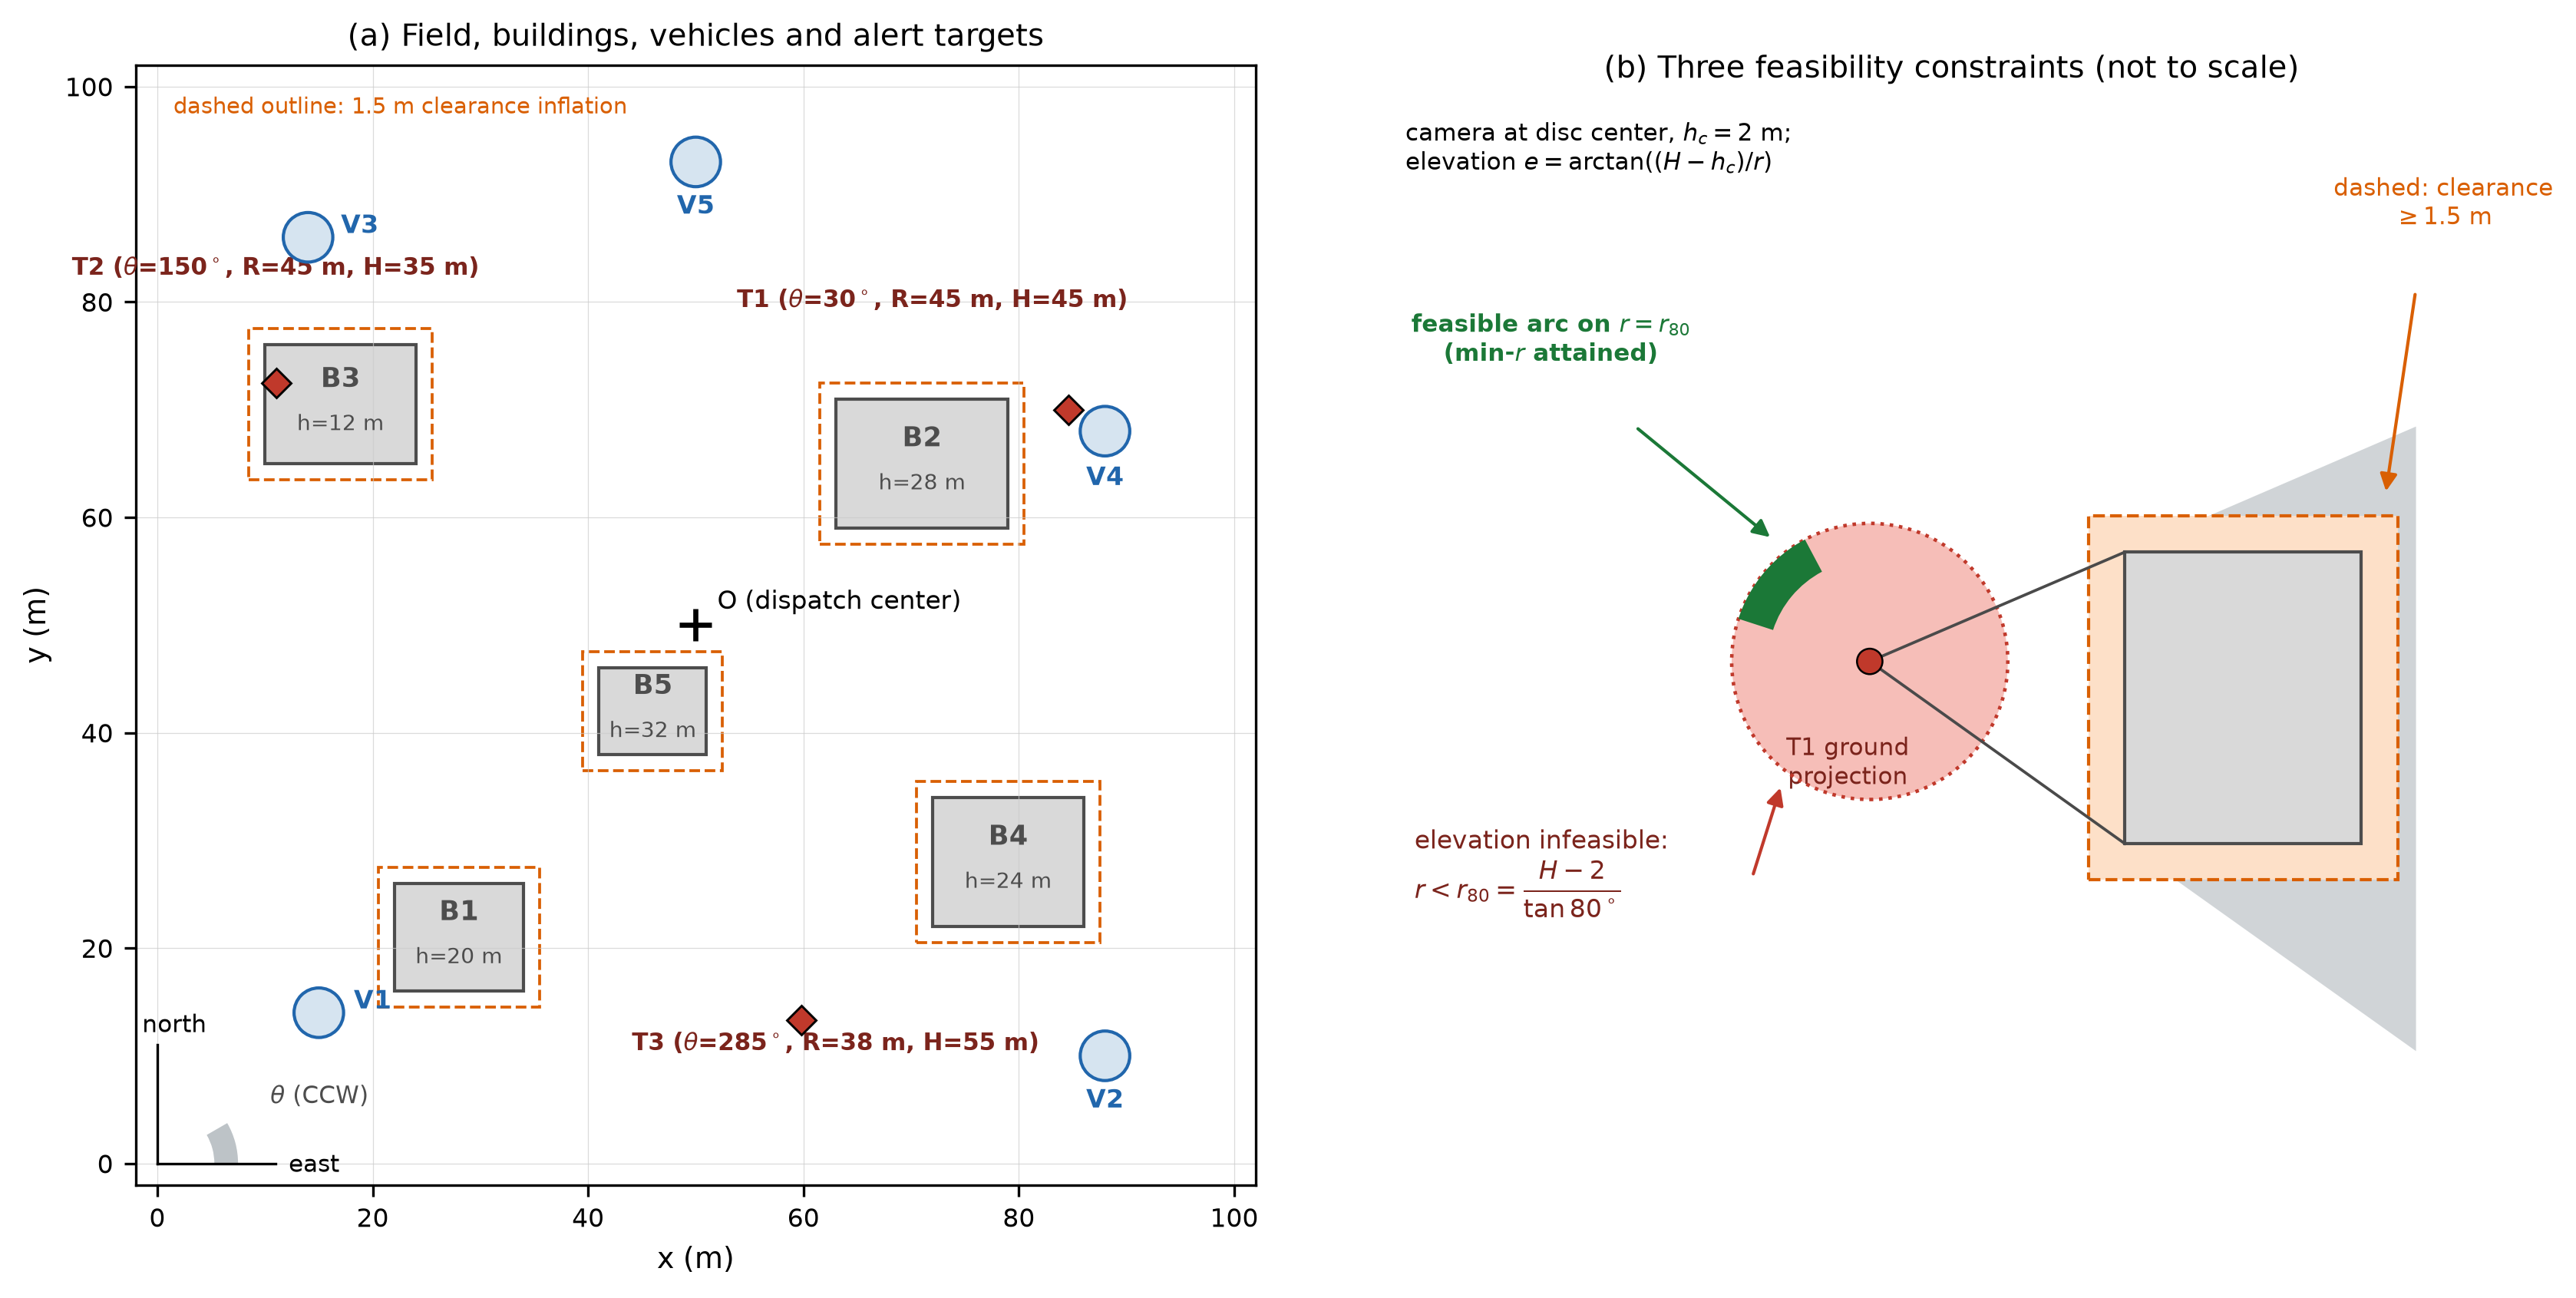
\includegraphics[width=0.62\textwidth]{fig_geometry_schematic.png}
\caption{(a) Field layout: buildings with heights, the $1.5$-m clearance inflation
(dashed), vehicles $V_1$--$V_5$ (blue) and alert targets (red diamonds).
(b) The three feasibility sieves around a target: elevation excludes $r<r_{80}$
(pink disc), an occlusion shadow (gray wedge), and the inflated footprint (orange).}
\label{fig:schematic}
\end{figure}

Figure~\ref{fig:schematic}b shows that the three constraints remove qualitatively
different disc centers---too close, hidden behind a building, or overlapping an
obstacle---so the observable region is the survivor set of three sieves. This dictates
the Q1 strategy: characterize each sieve analytically, intersect them numerically, and
audit the intersection with an independent method.

\subsection{Analysis of Question 1}

Question 1 asks for $\mathcal{F}_{T_1}$, the set of feasible camera positions for T1,
and the minimum target distance over it. Elevation alone yields the annulus
$r\ge r_{80}=7.5821\,\mathrm{m}$, so the real question is whether the $r_{80}$-circle
survives clearance and LOS anywhere---if so, the optimum is attained on a whole arc and
a tie-breaking rule becomes part of the model rather than an afterthought. We pair a
robust grid computation (for the required region map) with an analytic arc computation
on the $r_{80}$-circle (for the exact optimum), declaring the tie-break explicitly
(Section~\ref{sec:q1}).

\subsection{Analysis of Question 2(1)}

Question 2(1) is estimation theory wrapped in a discrete--continuous optimization:
choose 2 of 5 vehicles and one station per vehicle to minimize an accuracy metric under
a 30-s travel budget ($90\,\mathrm{m}$ geodesic). Bearing-only localization accuracy is
classical Fisher-information territory \cite{torrieri1984,aidala1979,kay1993}; the
problem adds feasibility---stations must lie in $\mathcal{F}_{T_2}$ and be reachable. We
adopt the root-mean-square position error $\mathrm{RMSE}=\sqrt{\operatorname{tr}C}$
(A-optimality) as primary metric---meters, comparable across pairs, directly
interpretable---with the determinant (error-ellipse area) and condition number
(anisotropy) of $C$ as diagnostics. The closed form
$\mathrm{RMSE}=\sigma_b\sqrt{d_1^2+d_2^2}/\sin\gamma$ turns the search into geometry:
the lower bound $\sigma_b\sqrt2\,r_{80}$ is attained iff both stations sit on the
$r_{80}$-circle at $\gamma=90^\circ$, reducing the continuous optimization to a
one-parameter family plus a tie-break---mirroring the structure discovered in Q1.

\subsection{Analysis of Question 2(2)}

Question 2(2) is a small-scale assign-and-sequence problem in the classical
deterministic-scheduling sense \cite{pinedo2023}: 3 alerts, 2 vehicles each, 5 vehicles,
so at least one vehicle serves two alerts; the objective is min--max on the latest
alert-start time. The combinatorial outer layer (who doubles, in which order, with which
partner) is exhaustively enumerable within the natural single-doubler family
($5\times3\times2\times4!/2=360$ structures), while the continuous inner layer (six
station coordinates) is handled by candidate screening plus best-response refinement;
both layers are evaluated by the same event-timeline simulator that Q4 reuses. We do
\emph{not} claim global optimality from enumeration alone: a valid lower bound
($3.873\,\mathrm{s}$, per-alert earliest starts ignoring resource sharing) and the
resulting gap are reported honestly. The required self-defined
\emph{nearest-assignment} baseline is defined as per-alert independent minimax station
choice with first-come--first-served assignment, so the comparison diagnoses exactly
which greedy shortcut costs how much.

\subsection{Analysis of Question 3}

Question 3 is a one-dimensional error-synthesis problem plus an inverse problem: three
independent Gaussian sources---vehicle-position error (variance growing with cumulative
travel $s$), gimbal zero bias ($0.8^\circ$) and control error ($0.6^\circ$)---enter the
pointing error $\Delta\psi$ additively to first order, so $\Delta\psi$ is Gaussian with
closed-form $\sigma_{tot}(s)$ and the reliability constraint
$P(|\Delta\psi|\le5^\circ)\ge0.95$ becomes a linear inequality in $(a,b)$ for the error
law $\sigma_{loc}(s)=a+bs$. The analytical chain is cheap to invert but rests on a
small-angle linearization; we validate it by deterministic quadrature of the exact
\texttt{atan2} angle law and exact-geometry Monte Carlo \cite{metropolis1949} (angle
wrapping, no linearization), and complement the Gaussian result with distribution-free
bounds (Chebyshev/Cantelli) to
show what normality buys. Q3 runs parallel to Q2 but feeds back a deployment insight:
the pointing-reliability limit at $r=40\,\mathrm{m}$ is compared with the separate
$90\,\mathrm{m}$ driving limit of Q2(1).

\subsection{Analysis of Question 4}

Question 4 extends the Q2(2) plan to a stochastic event stream: at $t=5\,\mathrm{s}$ a
new alert may appear (type a), one vehicle may fail (type b), and communications may be
interrupted until $t_{rec}$ (type c), singly or combined. The evaluation metric is
lexicographic---completion ratio $\eta=k/N$ first, then the latest start $t_{last}$
(capped at $60\,\mathrm{s}$ when any open alert can never start)---and the comparison is
against \emph{retaining} the original commands ($P_0$). A compact scenario family
(86 scenarios) covers the full parameter domain of (a) on a $12\times3$ grid, all five
failures of (b), multiple recovery times of (c), and worst-case combinations located by
a hard-sector probe; three strategies are evaluated---$P_0$ (retain), $P_1$
(event-triggered full re-optimization sharing Q2(2)'s machinery) and $P_2$
(an interpretable rule-based greedy)---in the spirit of dynamic multi-robot task
allocation under uncertainty \cite{choudhury2022,chakraa2023}. Pairing a proactive
optimizer with a rule-based fallback lets us attribute \emph{when} and \emph{why}
rescheduling pays---a value-boundary analysis rather than a single average number.

\begin{figure}[!htb]\centering
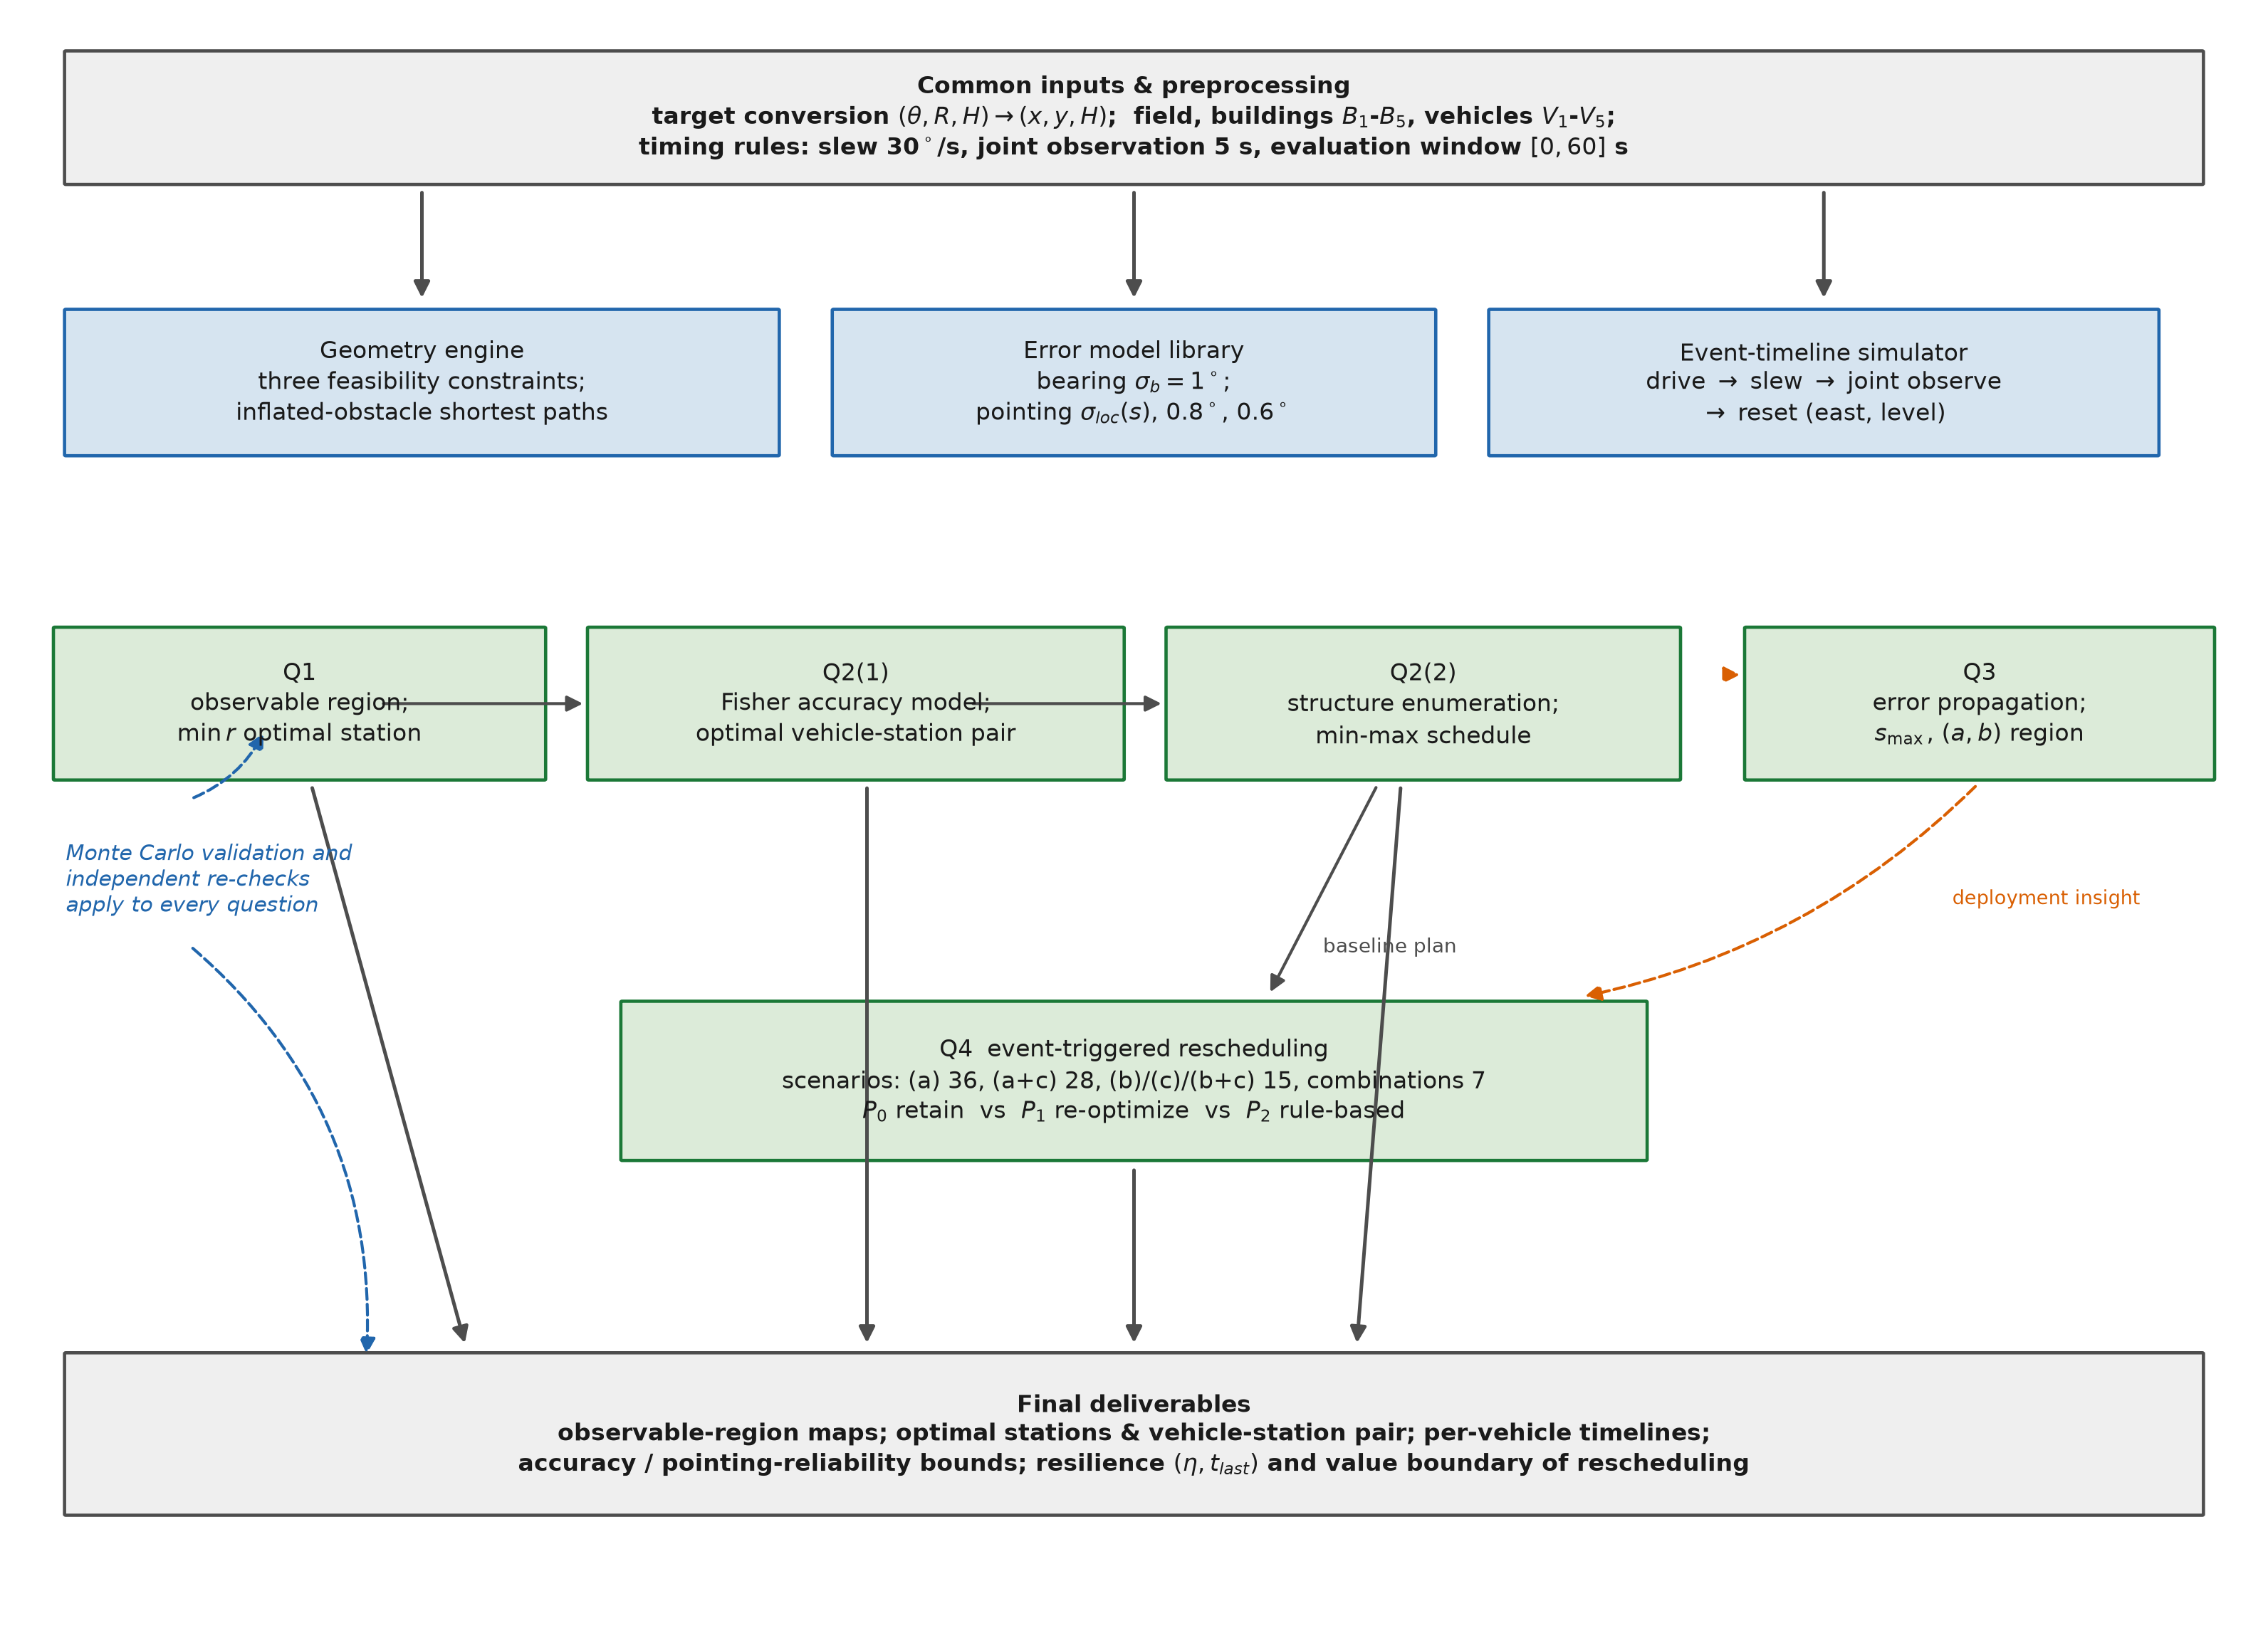
\includegraphics[width=0.56\textwidth]{fig_framework.png}
\caption{Overall technical route. Three shared engines (blue) serve all questions
(green); dashed arrows are cross-question transfers: Q3's deployment insight feeds the
schedule discussion, Q2(2)'s plan is Q4's baseline, and every question carries its own
Monte Carlo / independent re-check loop.}
\label{fig:framework}
\end{figure}

Figure~\ref{fig:framework} shows the whole pipeline. The two arrows into Q4---one solid
(baseline plan) and one dashed (deployment insight)---embody the framework's central
claim: scheduling decisions and error mechanics are two views of the same geometry, and
one shared simulator is what makes the Q4 comparison meaningful.

\subsection{Method-Selection Summary}

Table~\ref{tab:methodsel} consolidates, for each question, the candidate approaches
weighed against the selected one; the decisive criterion is always the metric the
problem statement itself asks for (feasible-region fidelity, localization accuracy,
latest alert start, pointing reliability, and the lexicographic $(\eta,t_{last})$
pair), and each selection is backed by evidence already reported in the corresponding
section---no untested alternative is claimed superior or inferior beyond what the
tables in Sections~\ref{sec:q1}--\ref{sec:q4} show.

\begin{table}[!htb]\centering\footnotesize
\setlength{\tabcolsep}{3.5pt}
\caption{Candidate approaches considered per question and the selection criterion.}
\label{tab:methodsel}
\begin{tabular}{p{0.065\textwidth}p{0.36\textwidth}p{0.22\textwidth}p{0.27\textwidth}}
\toprule
Q & Candidates weighed & Selected & Decisive reason \\
\midrule
Q1 & full grid enumeration; analytic $r_{80}$-circle arc audit; random feasible-set
sampling & grid map $+$ analytic arc audit & the map is required; the arc audit
\emph{certifies} that the bound $r_{80}$ is attained, which sampling cannot \\
Q2(1) & Fisher/CRLB metric; least-squares trilateration; weighted intersection
estimator & Fisher $\mathrm{RMSE}=\sqrt{\operatorname{tr}C}$ & closed form, attainable
lower bound, $\propto\sigma_b$ so the pair choice is noise-level free \\
Q2(2) & min--max makespan; total-completion-time; list scheduling & min--max epigraph
(Eq.~\eqref{eq:minmax}) & matches the required objective verbatim; total-time variants
optimize a different (unasked) quantity \\
Q3 & analytic linear chain; exact quadrature $+$ Monte Carlo; distribution-free bounds
& analytic chain $+$ full-geometry validation $+$ Chebyshev/Cantelli contrast & the chain
is directly invertible to the $(a,b)$ region; quadrature and MC quantify its approximation
error; the free bounds price the normality assumption \\
Q4 & $P_1$ enumeration $+$ coordinate descent; rule-based greedy ($P_2$); re-enumerate
everything at every event & event-triggered $P_1$ with $P_2$ fallback vs.\ $P_0$ &
lexicographic $(\eta,t_{last})$; the pairing attributes \emph{when} rescheduling pays
(the value boundary) \\
\bottomrule
\end{tabular}
\end{table}

\section{Assumptions and Justifications}

\begin{itemize}\setlength{\itemsep}{4pt}
\item \textbf{Assumption 1 (station--camera coincidence).} The station coordinate equals
the horizontal position of the camera, which sits at the center of the vehicle disc at
height $2\,\mathrm{m}$. \emph{Justification:} this is the problem's own convention; it
makes the 3-D sightline start at $(x_s,y_s,2)$ and all geometry two-dimensional in the
ground plane.
\item \textbf{Assumption 2 (travel times are visibility-graph shortest paths).} Vehicles
move at constant $3\,\mathrm{m}/\mathrm{s}$ along shortest paths in the corner-visibility
graph of obstacles inflated by $1.5\,\mathrm{m}$; turning costs no time. Path lengths so
computed are \emph{feasible upper bounds} of true geodesic minima, because a finite corner
graph may miss shorter curved routes; all feasibility verdicts (e.g.\ the 30-s budget)
are therefore conservative. \emph{Justification:} exact geodesics in a polygonal domain
require edge-stacking; the upper-bound reading keeps every reported schedule executable.
\item \textbf{Assumption 3 (error model and independence).} In Q2(1) the two bearing
measurement errors are independent $N(0,1^{\circ^2})$; in Q3 the three pointing error
sources (target position error with $\sigma_{loc}(s)=0.3+0.02s$ m per axis, gimbal zero
bias $0.8^\circ$, control error $0.6^\circ$) are independent and independent of Q2(1)'s
measurement error. \emph{Justification:} the distributions and parameters are given by
the problem; independence across the three Q3 sources is stated there, and Q2(1)/Q3
errors are different physical quantities (bearing measurement vs.\ pointing), used in
different questions only.
\item \textbf{Assumption 4 (small-angle linearization).} The position-induced pointing
error is linearized as $\Delta\psi_{loc}\approx\delta_\perp/r$ (radians), and the
$\pm180^\circ$ wrap never activates because $|\Delta\psi|\le5^\circ$ in the feasible
region. \emph{Justification:} the linearization's theoretical relative error at one
sigma is $5.6\times10^{-4}$, and the Monte Carlo validation of Section~\ref{sec:q3}
measures a worst-case deviation of $0.18$ percentage points in probability; wrap
probability is exactly zero at $s=80\,\mathrm{m}$.
\item \textbf{Assumption 5 (at most two task slots per vehicle).} Each vehicle executes
at most two alert tasks in Q2(2) and in every Q4 reschedule. \emph{Justification:} 6
slots and 5 vehicles imply a doubling vehicle; the cap keeps the structure family
finite (360 in the single-doubler core) and matches the found optimum, and in Q4 it
bounds the reassignment search consistently with the baseline plan.
\item \textbf{Assumption 6 (Q4 event conventions).} Disturbances occur at
$t=5\,\mathrm{s}$; for type-c outages the first moment new commands can take effect is
$t_{rec}$ (decision instant $t_{rec}$); an alert whose joint observation has
\emph{started} before the disturbance is regarded as completed and locked; a failed
vehicle leaves the field without obstructing others. \emph{Justification:} the locked
rule is Q4-08 of the problem; the decision-instant reading resolves the problem's dual
phrasing of outage length and recovery time, and is applied uniformly to all strategies.
\end{itemize}

\subsection{Notations}
Table~\ref{tab:notation} lists the symbols shared by all four models; symbols specific
to one question are defined at their first use in the text.

\begin{table}[!htb]\centering\small
\caption{Main symbols.}
\label{tab:notation}
\begin{tabular}{cl}
\toprule
Symbol & Meaning (unit) \\
\midrule
$\mathcal{F}_T$ & observable region: feasible camera positions for target $T$ (m) \\
$r$, $d_i$ & horizontal target distance; distance from station $i$ to target (m) \\
$r_{80}$ & $(H-2)/\tan80^\circ$: minimum admissible horizontal distance (m) \\
$e$ & gimbal elevation angle ($^\circ$), feasible $\in[-10^\circ,80^\circ]$ \\
$\theta$, $R$, $H$ & alert azimuth ($^\circ$), radius (m), height (m) \\
$B$, $\gamma$ & baseline length between the two stations (m); crossing angle ($^\circ$) \\
$\sigma_b$ & bearing measurement standard deviation ($^\circ$) \\
$C$, $\operatorname{tr}C$ & position-estimate covariance ($\mathrm{m}^2$) and its trace \\
$\mathrm{RMSE}$ & $\sqrt{\operatorname{tr}C}$: expected localization error (m) \\
$\tau_{slew}$, $\tau_{reset}$ & slew and reset times,
$\max(|\Delta\mathrm{pan}|,|\Delta\mathrm{tilt}|)/30^\circ\mathrm{/s}$ (s) \\
$t^{start}_a$ & joint-observation start time of alert $a$ (s) \\
$\tau$ & min--max epigraph variable / rescheduling decision instant (s) \\
$s$ & cumulative travel distance of a vehicle since departure (m) \\
$\sigma_{loc}(s)$ & per-axis target-position error std, $0.3+0.02s$ (m) \\
$\Delta\psi$, $\sigma_{tot}$ & pointing error ($^\circ$) and its total std ($^\circ$) \\
$k$, $N$, $\eta$ & observed alerts, total alerts, completion ratio $k/N$ \\
$t_{last}$ & latest observation start, capped at $60\,\mathrm{s}$ (s) \\
$P_0$, $P_1$, $P_2$ & retain / re-optimize / rule-based strategies in Q4 \\
\bottomrule
\end{tabular}
\end{table}

\section{Model Establishment and Solution}

\subsection{Question 1: Observable Region and Optimal Station}\label{sec:q1}

\subsubsection{Model}

Let $p=(x,y)$ be a candidate station (the vehicle-disc center) and $T$ an alert with
ground projection $T_p$ and height $H$. The observable region
$\mathcal{F}_T=\mathcal{C}_{\mathrm{clr}}\cap\mathcal{C}_{\mathrm{los}}\cap\mathcal{C}_{\mathrm{elev}}$
is the intersection of three constraint sets.

\textbf{(i) Clearance.} The disc of radius $1.5$ m must not penetrate the field boundary
or any building footprint $B_j=[x_{j0},x_{j1}]\times[y_{j0},y_{j1}]$:
\begin{equation}\label{eq:clr}
1.5\le x,y\le98.5,\qquad
\operatorname{dist}\bigl(p,B_j\bigr)=\Bigl\|\bigl(|p-c_j|-s_j\bigr)^{+}\Bigr\|\ge1.5,
\end{equation}
where $c_j$ and $s_j=(s_{jx},s_{jy})$ are the center and half-sizes of $B_j$; equivalently
$p$ must lie outside the Minkowski inflation of every footprint by $1.5$ m
(Fig.~\ref{fig:schematic}b, orange).

\textbf{(ii) Line of sight.} The sightline from $(p,2)$ to $(T_p,H)$ is blocked by
building $B_j$ (height $h_j$) if its horizontal projection meets $B_j$ while its height
there is at most $h_j$; with $\lambda\in[0,1]$ parametrizing the horizontal segment
$p\to T_p$,
\begin{equation}\label{eq:los}
\exists\,\lambda:\; q(\lambda)\in B_j,\;\; z(\lambda)=2+(H-2)\lambda\le h_j ,
\end{equation}
and \emph{tangency counts as blocked} (closed-set test). Because $H>h_j$ for all $j$,
blocking requires $\lambda\le(h_j-2)/(H-2)$: only stations on the far side of a building,
within the ground shadow wedge of the target, lose their sightline.

\textbf{(iii) Elevation.} With $r=\|p-T_p\|$ the horizontal distance and camera height
$2\,\mathrm{m}$, the elevation angle $e=\arctan\bigl((H-2)/r\bigr)$ must lie in
$[-10^\circ,80^\circ]$. Since $H>2$, $e>0$ always, so the binding condition is
\begin{equation}\label{eq:elev}
r\;\ge\;r_{80}\;\triangleq\;\frac{H-2}{\tan 80^\circ}.
\end{equation}

The optimization problem is
\begin{equation}\label{eq:q1opt}
\min_{p\in\mathcal{F}_{T}}\; r(p)=\|p-T_p\| .
\end{equation}
Equation~\eqref{eq:elev} immediately gives the \emph{a priori lower bound} $r\ge r_{80}$;
the optimum attains it iff the circle $\|p-T_p\|=r_{80}$ has a nonempty feasible arc.

\subsubsection{Algorithm}

The region is computed on a $0.1$-m grid over $[1.5,98.5]^2$ (a standard rasterization
approach \cite{deberg2008}): each grid point is tested against
Eq.~\eqref{eq:clr}--\eqref{eq:elev} (LOS uses exact segment--rectangle intersection with
closed endpoints), components are labeled, and the boundary is refined by a $0.02$-m
local search around sign changes. Independently, the \emph{critical circle}
$\|p-T_p\|=r_{80}$ is traced analytically: each station azimuth $\phi$ is tested against
clearance and LOS, yielding the feasible arc(s) with the cause of each endpoint---this
audit certifies whether Eq.~\eqref{eq:q1opt}'s lower bound is attained.

Tie-breaking over the optimal arc is declared as part of the model, in priority order:
\textbf{(1)} a hard clearance margin of $0.10\,\mathrm{m}$ beyond the $1.5$-m vehicle
buffer (boundary robustness); \textbf{(2)} minimize the designated vehicle's
\emph{mission-cycle time} from its standby position---travel $+$ slew $+$ 5-s joint
observation $+$ reset $=$ travel $+2\tau+5\,\mathrm{s}$, since the reset mirrors the
slew---with the nearest standby vehicle designated as the observer for each target
(V4 for T1, V3 for T2, V2 for T3); \textbf{(3)} ties: larger clearance margin, then
distance to the dispatch center $O$, then azimuth. On the $r_{80}$-arc every station
has $\mathrm{tilt}=80^\circ$, so $\tau=2.667\,\mathrm{s}$ whenever
$|\mathrm{wrap}(\mathrm{pan})|\le80^\circ$ and the cycle reduces to
$\mathrm{travel}+10.33\,\mathrm{s}$---the rule selects the arc point closest to the
designated vehicle.

\subsubsection{Results}

\begin{table}[!htb]\centering\footnotesize\setlength{\tabcolsep}{4pt}
\caption{Observable regions and min-$r$ optimal stations (grid $0.1$ m; angles on the
$r_{80}$-circle measured from the target projection, CCW from east). Stations are
reported to six decimals---see the printed-precision note below.}
\label{tab:q1opt}
\begin{tabular}{lccc}
\toprule
 & T1 & T2 & T3 \\
\midrule
$r_{80}$ (m) & 7.5821 & 5.8188 & 9.3453 \\
feasible arc on $r_{80}$-circle & $[236.90^\circ,160.74^\circ]$ & $[59.66^\circ,244.24^\circ]$ & full circle \\
arc span / endpoint cause & $283.84^\circ$ / clearance & $184.58^\circ$ / LOS, clearance & $360^\circ$ / -- \\
area of $\mathcal{F}_T$ (m$^2$) & 5628.7 & 6432.5 & 5484.8 \\
connected components & 1 & 1 & 1 \\
designated vehicle & V4 & V3 & V2 \\
optimal station $(x,y)$ & $(83.324405,\,62.533128)$ & $(10.018434,\,78.230390)$ & $(58.212324,\,4.091465)$ \\
pan / tilt ($^\circ$) & $80.0\,/\,80.0$ & $280.0\,/\,80.0$ & $80.0\,/\,80.0$ \\
slew $=$ reset (s) & 2.667 & 2.667 & 2.667 \\
mission cycle (s) & 12.731 & 13.243 & 20.456 \\
clearance beyond buffer (m) & 2.824 & 0.730 & 2.591 \\
\bottomrule
\end{tabular}
\end{table}

The minimum $r^{*}=r_{80}$ is attained for all three targets: T1's critical circle
survives over a $283.84^\circ$ arc, T2's over $184.58^\circ$ (one end LOS-limited, the
other clearance-limited), and T3's entire circle is feasible ($H=55$ clears every
building). Rule (2) selects, on each arc, the point closest to the designated
vehicle's standby position: V4 for T1 (azimuth $260.0^\circ$), V3 for T2
($100.0^\circ$---the edge of the constant-slew sector, where travel toward V3 is
shortest), and V2 for T3 ($260.0^\circ$). Table~\ref{tab:q1opt} lists the stations;
all three sit \emph{exactly} on the $80^\circ$ elevation boundary---inherent to the
objective, since $Q=1/r$ is maximal only on the $r_{80}$-circle---feasible on the
closed set, with robustness examined in Section~\ref{sec:sens}.

\emph{Printed precision.} The table reports six decimals deliberately: all three
stations sit at exactly $80.000000^\circ$ elevation (T2 additionally at the edge of
the constant-slew sector), so a four-decimal rounding can push the printed point
$10^{-5}\,\mathrm{m}$ inside the elevation boundary and a strict re-check would---wrongly---reject
it. Deployments should use the six-decimal values (or the exact construction
$p^{*}=T_p+r_{80}(\cos\varphi^{*},\sin\varphi^{*})$); every reported station carries
the $0.10$-m clearance margin of rule (1), and a $0.5^\circ$ step along the arc into
the interior is strictly feasible in both of our implementations with \emph{identical}
$Q$, since every arc point has $r=r_{80}$.

\emph{Alternative tie-break (nearest to $O$).} An earlier draft declared a different
rule---minimize the distance to the dispatch center over the arc---which selects
$(80.500050,\,63.648619)$ for T1 at the clearance-tangent arc endpoint (mission cycle
$13.22\,\mathrm{s}$, clearance margin $0.0004\,\mathrm{m}$). Both rules are reasonable
under the problem statement; the mission-cycle rule is adopted because the problem's
objective is \emph{rapid} deployment and it matches the convention used in Q2(1), and
the coexistence of the two outcomes on the same arc---identical $Q$, cycle differing
by $0.49\,\mathrm{s}$---confirms the flat-optimum structure.

\begin{figure}[!htb]\centering
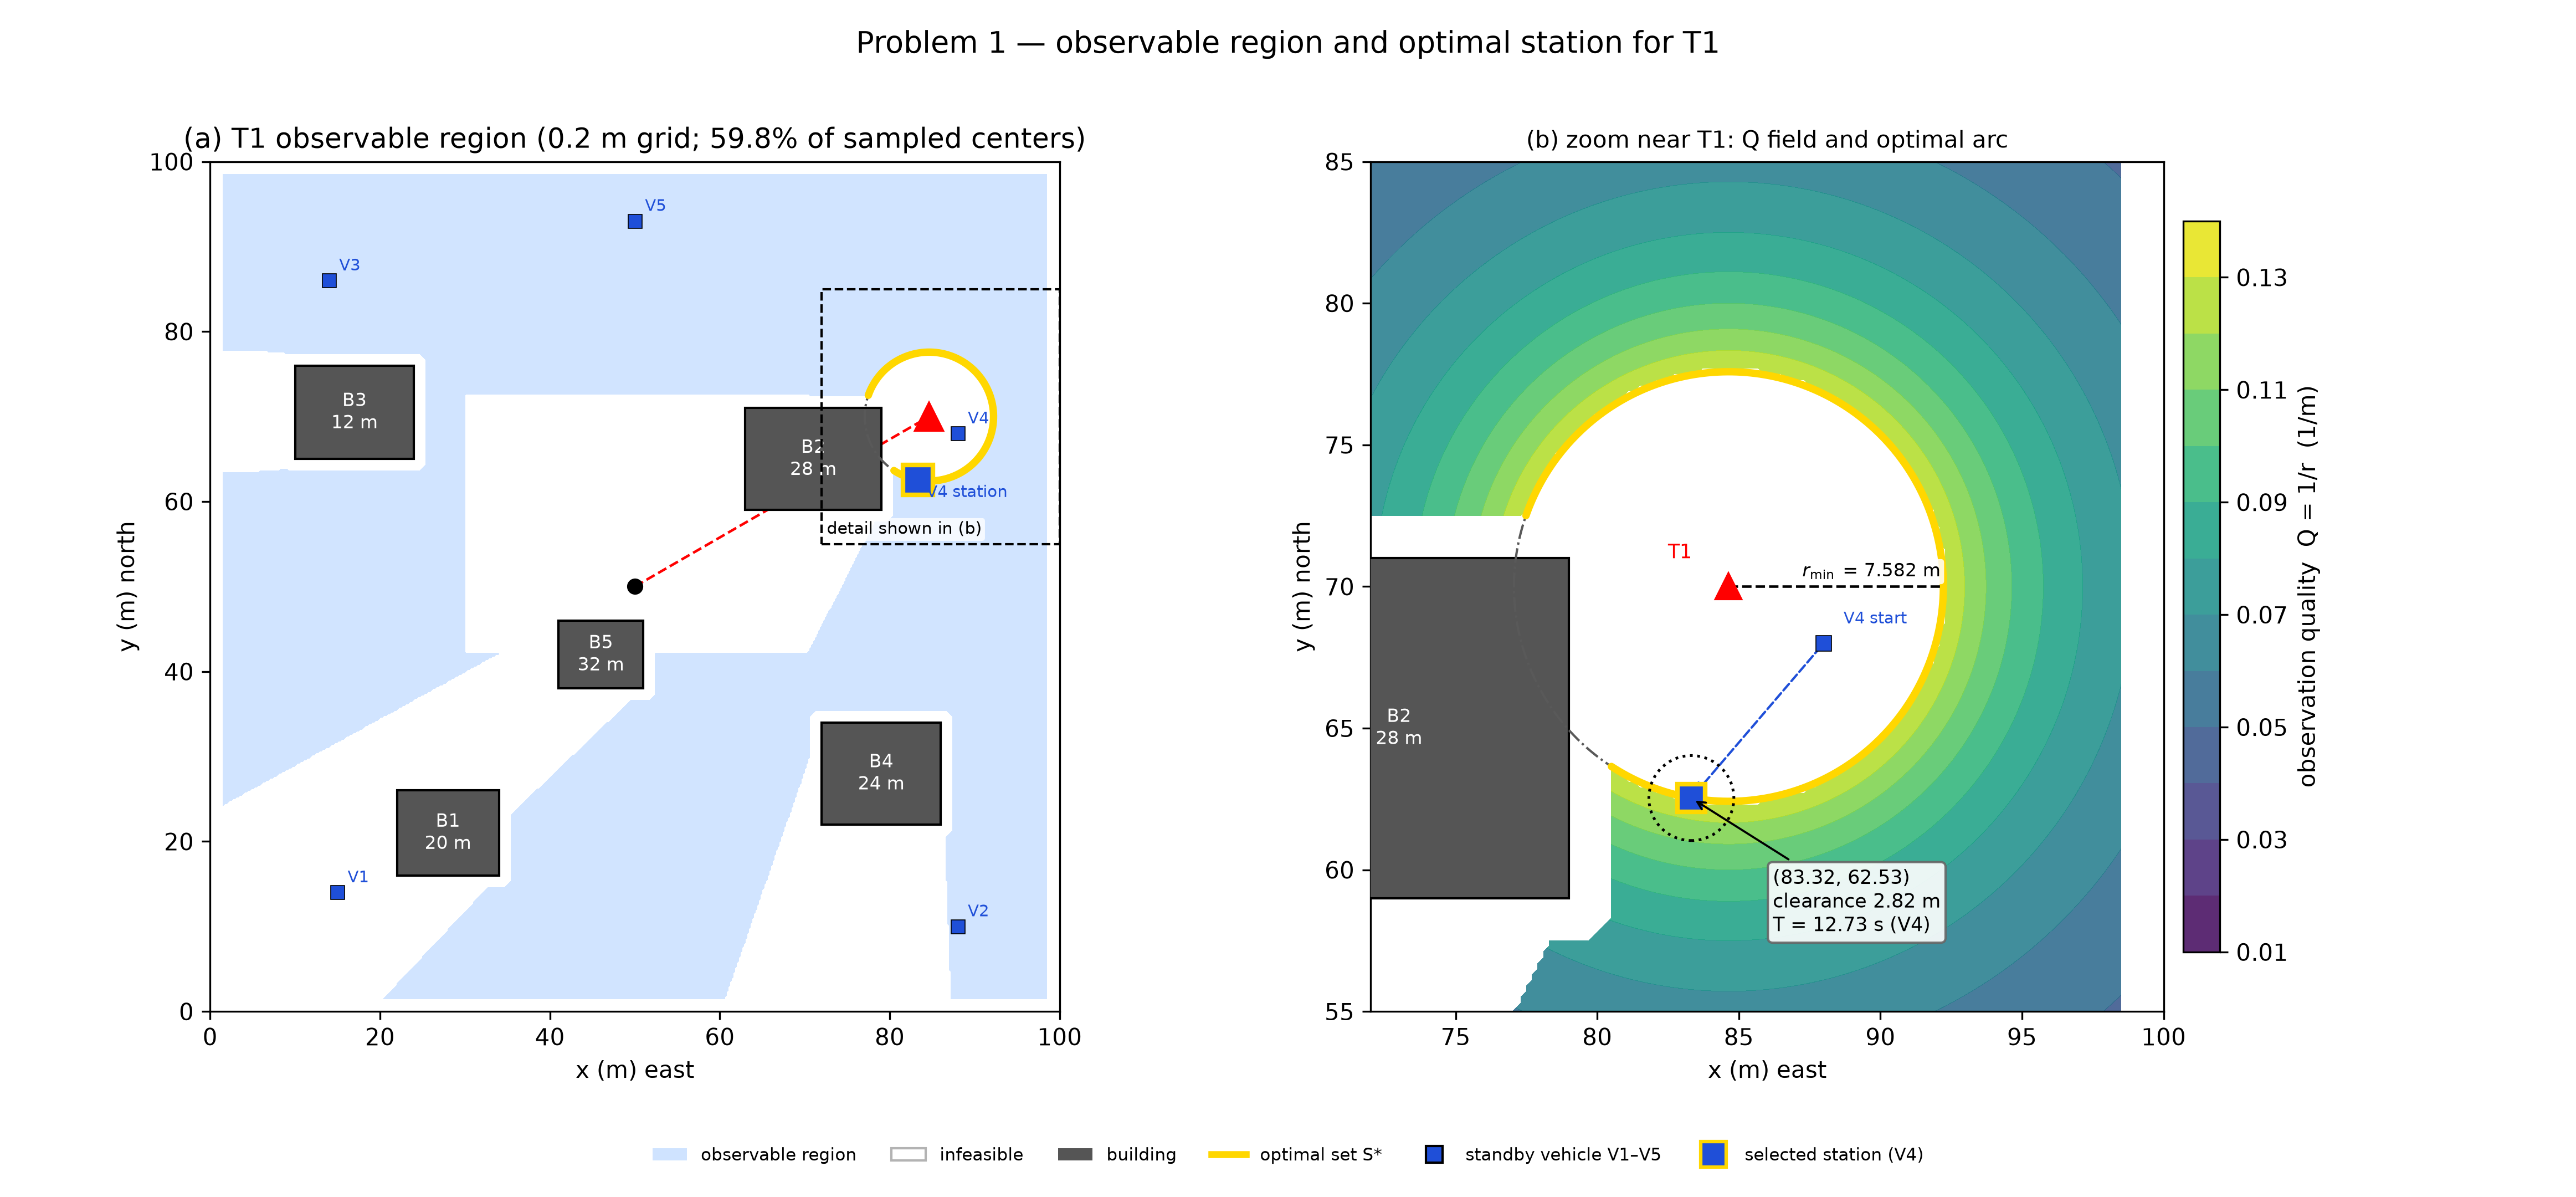
\includegraphics[width=\textwidth]{fig_q1_T1_region.png}
\caption{T1 observable region (left: $0.2$-m raster, $59.8\%$ of sampled centers;
right: zoom on the quality field $Q=1/r$). The gold arc is the optimal set
$S^{*}$---every point of it attains $r^{*}=7.5821$ m ($Q^{*}=0.1319$ m$^{-1}$); the
blocked sector ($160.74^\circ$--$236.90^\circ$) is the $B_2$ shadow. The selected
station for the designated vehicle V4 (square, with its $1.5$-m disk) carries a
$2.82$-m clearance margin, and the annotation reports V4's full mission cycle.}
\label{fig:q1t1}
\end{figure}
\begin{figure}[!htb]\centering
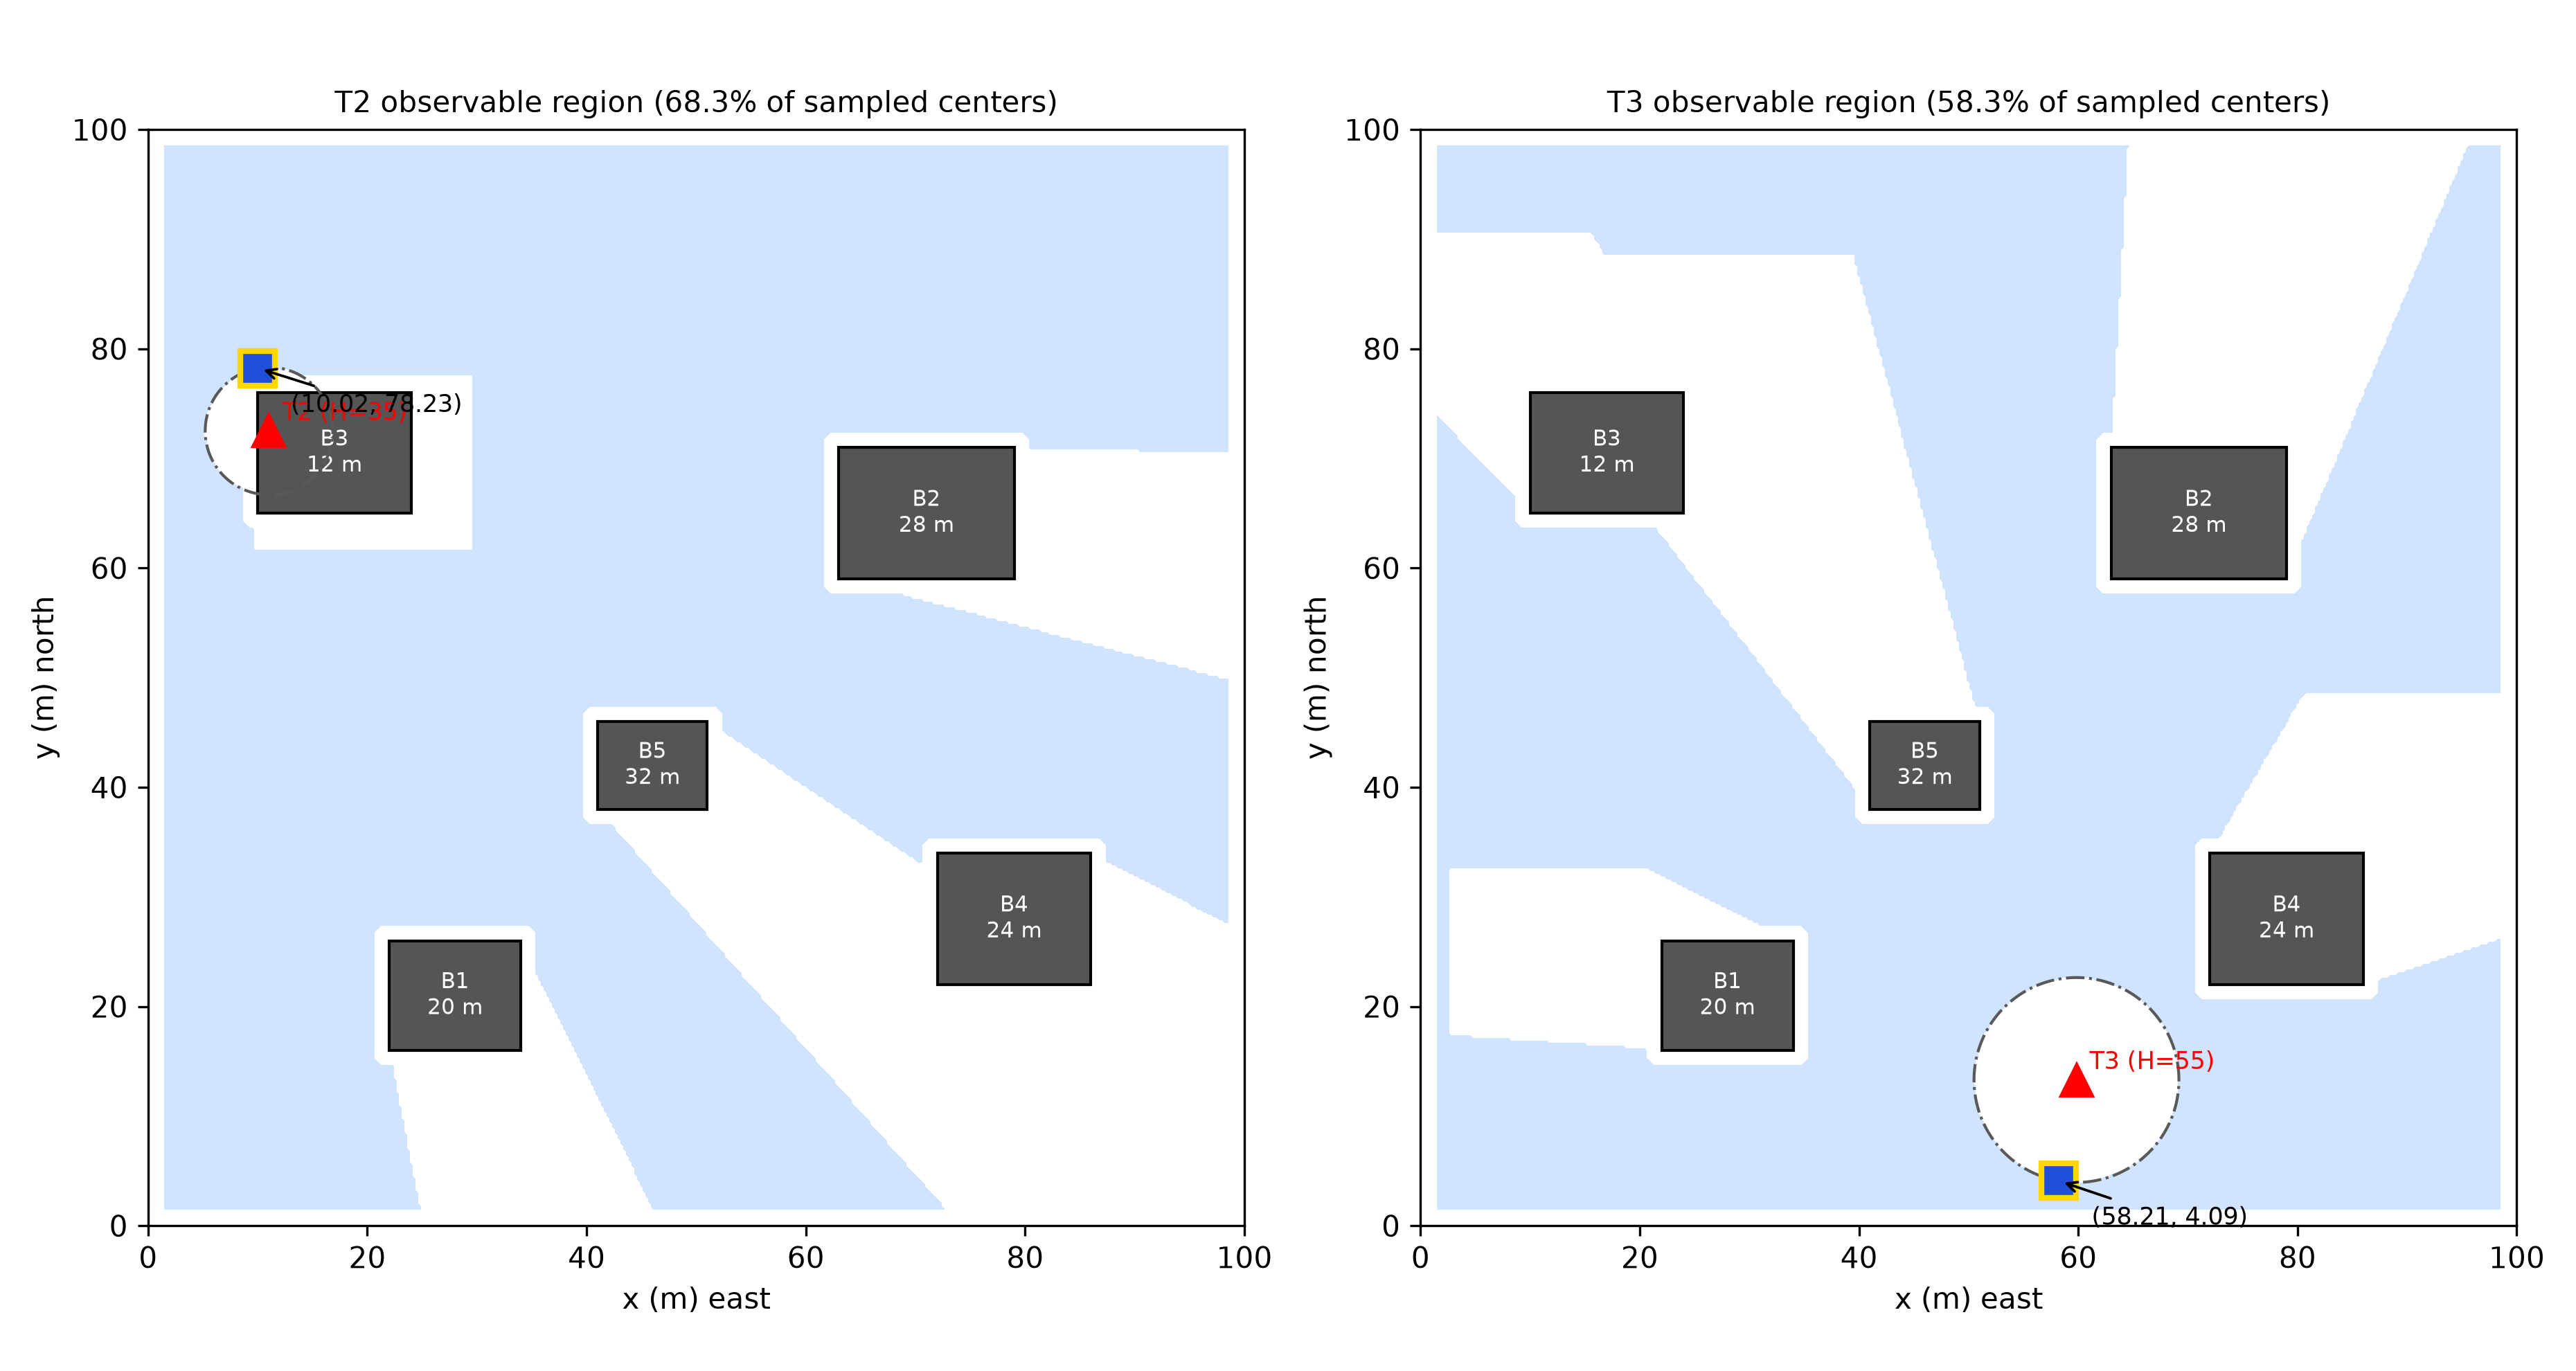
\includegraphics[width=0.78\textwidth]{fig_q1_T2_T3_regions.png}
\caption{Observable regions of T2 (left) and T3 (right) at $0.25$-m resolution with
the selected stations. T2 is pinched by $B_3$'s shadow and clearance, while T3 (the
tallest target) keeps its full elevation circle; all three selected stations
lie on the elevation circle closest to their designated vehicle.}
\label{fig:q1t23}
\end{figure}

Figures~\ref{fig:q1t1} and~\ref{fig:q1t23} confirm the mechanism predicted in Section~2.2: elevation removes
a disc around each target, clearance removes collars around buildings and the boundary,
and LOS removes wedges only on the far side of buildings relative to the (high)
target---for T2 the wedge is large because the target hovers low ($35$ m) above $B_3$,
while T3 loses nothing to LOS. The regions are all single components of areas
$5.5$--$6.4\times10^3\,\mathrm{m}^2$ ($55$--$64\%$ of the field), so station placement
has ample freedom for the later questions.

\subsubsection{Validation}

Four checks close Q1. First, at each chosen station all three constraints were
re-evaluated pointwise: elevations equal exactly $80.000000^\circ$ (the objective
boundary, inherent to $Q=1/r$), and the clearance margins of rule (1) are
$2.82/0.73/2.59\,\mathrm{m}$ beyond the buffer for T1/T2/T3, as designed. Second,
halving and doubling the grid resolution changes the region areas by at most $0.23\%$
(T1: $5628.7\,\mathrm{m}^2$ at $0.1$ m, $5619.6$ at $0.05$ m, $5607.8$ at $0.2$ m), so
the reported areas are resolution-stable. Third, the analytic critical-circle trace
reproduces the grid's inner (elevation) boundary and its feasible arcs exactly,
certifying that Eq.~\eqref{eq:q1opt}'s lower bound is genuinely attained rather than
grid-limited. \emph{Conclusion: the region computation and the optimum are mutually
consistent, and the optimum is exact on the continuous feasible set.}

\subsection{Question 2(1): Accuracy Model and Optimal Vehicle--Station Pair}\label{sec:q21}

\subsubsection{Model}

Two vehicles $i=1,2$ at stations $s_i$ observe T2 (projection $T_p$, height $H$) with
bearing errors $\varepsilon_i\sim N(0,\sigma_b^2)$, $\sigma_b=1^\circ$, independent---the
textbook bearings-only measurement model \cite{torrieri1984,kay1993}:
\begin{equation}\label{eq:meas}
\phi_i=\operatorname{atan2}\bigl(T_y-s_{iy},\,T_x-s_{ix}\bigr)+\varepsilon_i .
\end{equation}
Linearizing Eq.~\eqref{eq:meas} at the true position, each bearing constrains the
position along the unit normal $n_i$ of its sightline, with sensitivity $1/d_i$ where
$d_i=\|s_i-T_p\|$:
\begin{equation}\label{eq:fisher}
I=\sigma_b^{-2}\sum_{i=1}^{2}\frac{n_i n_i^{\mathsf T}}{d_i^{2}},\qquad
C=I^{-1} .
\end{equation}
For the $2\times2$ Gram matrix $G=\sum_i n_i n_i^{\mathsf T}/d_i^2$ one has
$\operatorname{tr}G=d_1^{-2}+d_2^{-2}$ and $\det G=\sin^2\gamma/(d_1^2d_2^2)$, where
$\gamma$ is the crossing angle of the two sightlines; hence
\begin{equation}\label{eq:rmse}
\operatorname{tr}C=\frac{\operatorname{tr}G}{\det G}\,\sigma_b^{2}
=\sigma_b^{2}\,\frac{d_1^{2}+d_2^{2}}{\sin^{2}\gamma},
\qquad
\mathrm{RMSE}=\sqrt{\operatorname{tr}C}
=\sigma_b\,\frac{\sqrt{d_1^{2}+d_2^{2}}}{\sin\gamma}.
\end{equation}
Equation~\eqref{eq:rmse} is the requested accuracy law in one line: the baseline $B$
acts through the geometry linking $(d_1,d_2,\gamma)$
($B^2=d_1^2+d_2^2-2d_1d_2\cos\gamma$), the crossing angle enters as $1/\sin\gamma$.
Elevation Eq.~\eqref{eq:elev} forces $d_i\ge r_{80}=5.8188\,\mathrm{m}$ for T2, so
\begin{equation}\label{eq:lb}
\mathrm{RMSE}\;\ge\;\sigma_b\sqrt{2}\;r_{80}=0.14362\,\mathrm{m},
\end{equation}
with equality \emph{iff} $\gamma=90^\circ$ and $d_1=d_2=r_{80}$: both stations on the
$r_{80}$-circle, separated by a $90^\circ$ arc as seen from the target (perpendicular
sightlines). Under the hard operating margins of Assumption~7 (clearance
$\ge0.10\,\mathrm{m}$ beyond the $1.5$-m buffer, elevation $\le79.9^\circ$), the
smallest admissible radius is $r_{80}+0.10\,\mathrm{m}=5.9188\,\mathrm{m}$, so the
margin-compliant optimum is
$\sigma_b\sqrt2\,(r_{80}+0.10)=0.146092\,\mathrm{m}$---$1.73\%$ above the bound;
relaxing the margins to zero recovers Eq.~\eqref{eq:lb} exactly. We adopt
$\mathrm{RMSE}=\sqrt{\operatorname{tr}C}$ (A-optimality, meters) as primary metric: it
is proportional to $\sigma_b$, so the optimal pair is independent of $\sigma_b$;
$\det C$ (D-optimality) and $\operatorname{cond}C$ are secondary diagnostics.

Feasibility: station $s_i$ must lie in $\mathcal{F}_{T_2}\cap\mathcal{R}_i$, where
$\mathcal{R}_i$ is the $90$-m geodesic disc of vehicle $i$ (30\,s $\times$
$3\,\mathrm{m}/\mathrm{s}$, Assumption~2). The optimization is
\begin{equation}\label{eq:q21opt}
\min_{\{i,j\}\subset\{1..5\}}\;\min_{s_i\in\mathcal{F}_{T_2}\cap\mathcal{R}_i,\;
s_j\in\mathcal{F}_{T_2}\cap\mathcal{R}_j}\;
\sigma_b\frac{\sqrt{d_i^{2}+d_j^{2}}}{\sin\gamma(s_i,s_j)} .
\end{equation}

\subsubsection{Algorithm}

Outer layer: all $\binom{5}{2}=10$ vehicle pairs. Inner layer, per pair: a
hard-constrained scan of the analytic $90^\circ$ family---stations at target-azimuth
$\phi$ and $\phi+90^\circ$ (perpendicular sightlines; a $\phi+180^\circ$ pair would be
collinear and degenerate) on the operating circles
$r\in\{r_{80}+0.10,\,+0.12,\,+0.15,\,+0.20\}\,\mathrm{m}$---with the Assumption~7
margins enforced (clearance $\ge0.10\,\mathrm{m}$ beyond the buffer, elevation
$\le79.9^\circ$), $\phi$ scanned at $0.1^\circ$ and refined locally at
$0.005^\circ$/$0.002\,\mathrm{m}$; for each $\phi$ both assignments of the two
stations to $\{V_i,V_j\}$ are evaluated, and every candidate must satisfy travel
$\le30\,\mathrm{s}$ on visibility-graph paths (Fig.~\ref{fig:q2reach}). Ties in
RMSE---at the $1$-mm reporting granularity every margin-compliant radius in the band
rounds to the same value---are broken by the declared secondary criterion: the
two-vehicle \emph{mission-completion time}
$\max_i(t_i+\tau_i)+5+\max_i(\tau_i)$ (consistent with Q1's rule and the problem's
rapid-deployment objective), then total travel, then midpoint distance to $O$, then
azimuth. Pairs whose family scan is infeasible everywhere under the margins are
marked infeasible.

\begin{figure}[!htb]\centering
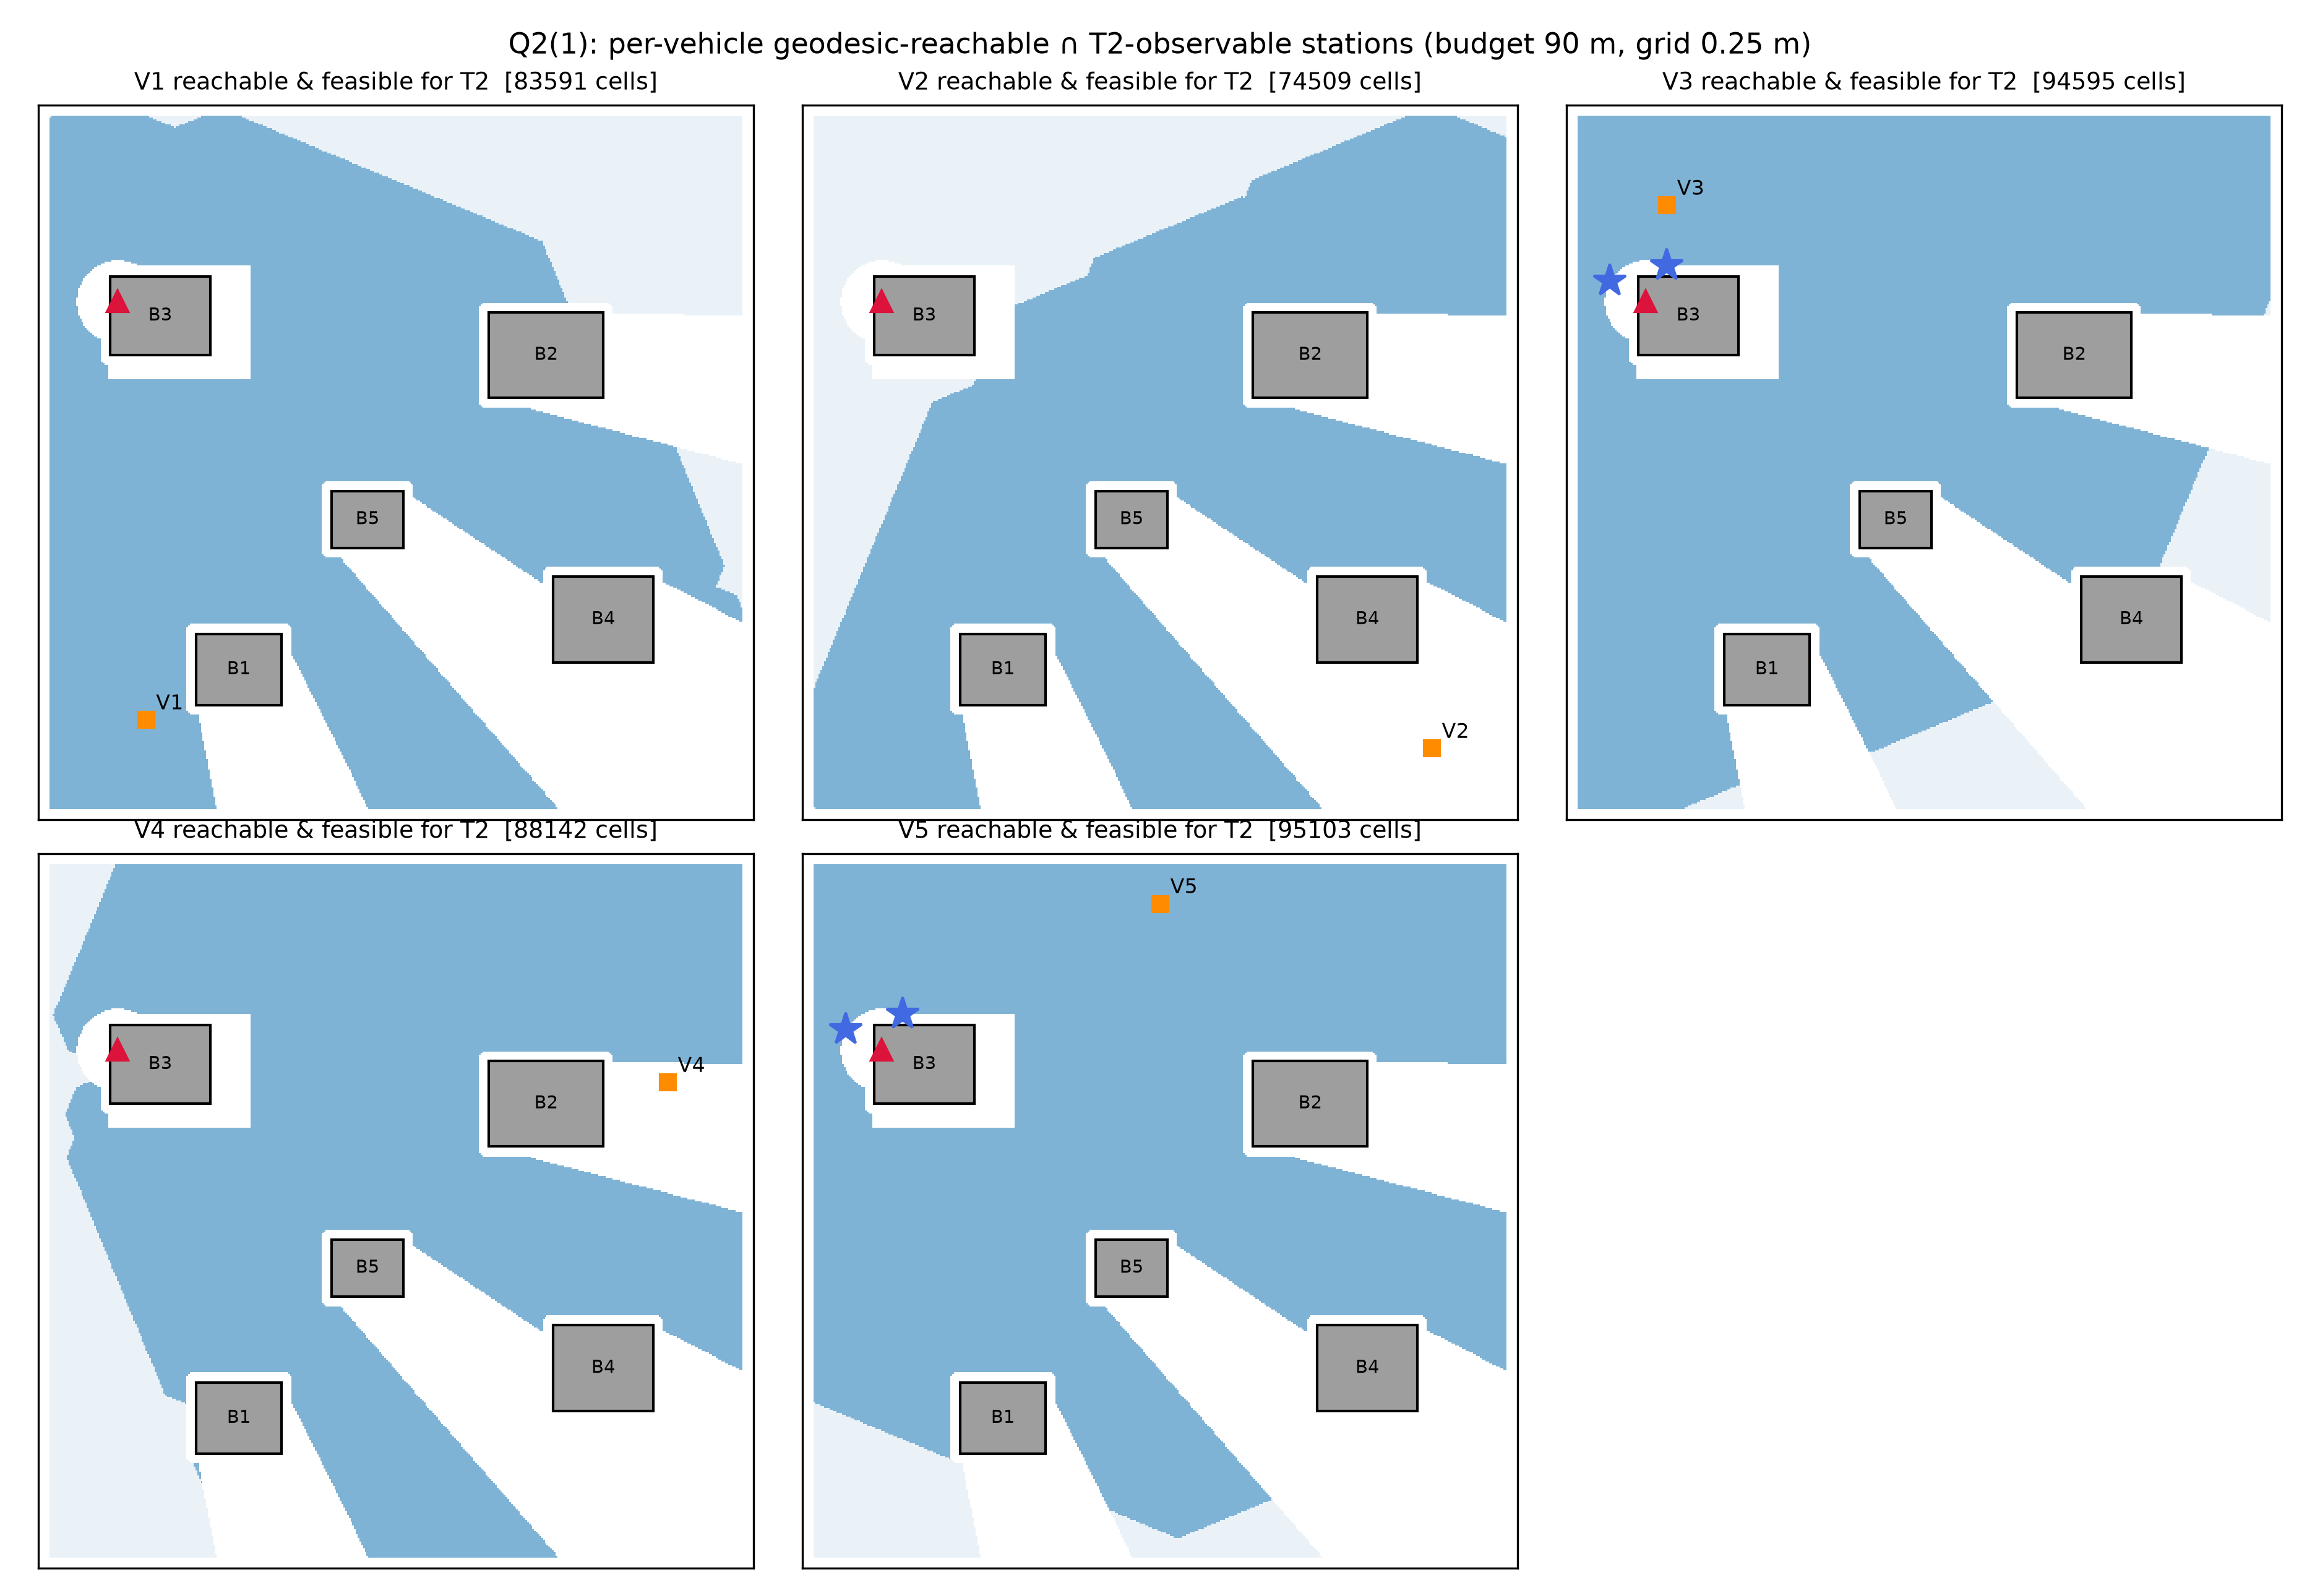
\includegraphics[width=0.55\textwidth]{fig_q2_1_reachability.png}
\caption{Reachable sets ($\le90$-m geodesic) intersected with $\mathcal{F}_{T_2}$ for the
five vehicles. V2's intersection is by far the poorest, foreshadowing its exclusion from
every competitive pair.}
\label{fig:q2reach}
\end{figure}

\subsubsection{Results}

\begin{table}[!htb]\centering\small
\setlength{\tabcolsep}{4.5pt}
\caption{Margin-compliant optimum by vehicle pair ($r=r_{80}+0.10$ m,
$\gamma=90^\circ$ and $B=8.370$ m for every pair; travels within the 30-s budget).
V2-containing pairs have no margin-compliant candidate within the budget and are
omitted.}
\label{tab:q21pairs}
\begin{tabular}{ccccc}
\toprule
Pair & RMSE (m) & $r$ (m) & total travel (s) & mission (s) \\
\midrule
(3,5) & 0.14609 & 5.9188 & 19.88 & 24.53 \\
(1,3) & 0.14609 & 5.9188 & 22.43 & 28.20 \\
(1,5) & 0.14609 & 5.9188 & 33.86 & 28.20 \\
(3,4) & 0.14609 & 5.9188 & 32.17 & 36.83 \\
(4,5) & 0.14609 & 5.9188 & 43.57 & 36.83 \\
(1,4) & 0.14609 & 5.9188 & 45.93 & 36.83 \\
\bottomrule
\end{tabular}
\end{table}

Table~\ref{tab:q21pairs} shows the same stratification as the unconstrained scan:
every pair excluding V2 reaches the margin-compliant optimum
$0.14609\,\mathrm{m}$ ($+1.73\%$ over the bound), while the four V2-containing pairs
have \emph{no} margin-compliant candidate within the travel budget at all---their
reachable intersection with $\mathcal{F}_{T_2}$ (Fig.~\ref{fig:q2reach}) is the
poorest, and under the unconstrained scan they stagnated near $0.30\,\mathrm{m}$
($2.1\times$ the bound). The mission-time tie-break selects \textbf{V3+V5}
(mission $24.53\,\mathrm{s}$ vs.\ $28.20$--$36.83\,\mathrm{s}$ for the other five);
the chosen five-fold output is consolidated in Table~\ref{tab:q21chosen}:

\begin{table}[!htb]\centering\small
\caption{Required five-fold output for the chosen vehicle--station pair.}
\label{tab:q21chosen}
\begin{tabular}{lc}
\toprule
Quantity & Value \\
\midrule
Vehicle pair & V3 $+$ V5 \\
Station of V3 / travel & $(5.203609,\;71.451873)$ / $5.667\,\mathrm{s}$ ($17.00\,\mathrm{m}$) \\
Station of V5 / travel & $(9.980729,\;78.325247)$ / $14.208\,\mathrm{s}$ ($42.62\,\mathrm{m}$) \\
Baseline $B$ / crossing angle $\gamma$ & $8.3704\,\mathrm{m}$ / $90.00^\circ$ \\
RMSE $=\sqrt{\operatorname{tr}C}$ & $0.146092\,\mathrm{m}$ ($+1.73\%$ over the margin-free bound) \\
$\det C$ / condition number & $1.139\times10^{-4}\,\mathrm{m}^4$ / $1.000$ \\
$1\sigma$ error-ellipse axes & $0.10330\,\mathrm{m}$ (isotropic) \\
$\mathrm{CEP}_{50}$ & $0.1216\,\mathrm{m}$ (Rayleigh) \\
Operating margins & clearance $3.30/0.83\,\mathrm{m}$ beyond buffer; elevation $79.83^\circ$ \\
Observation start / mission completion & $16.869\,\mathrm{s}$ / $24.530\,\mathrm{s}$ \\
\bottomrule
\end{tabular}
\end{table}

\begin{figure}[!htb]\centering
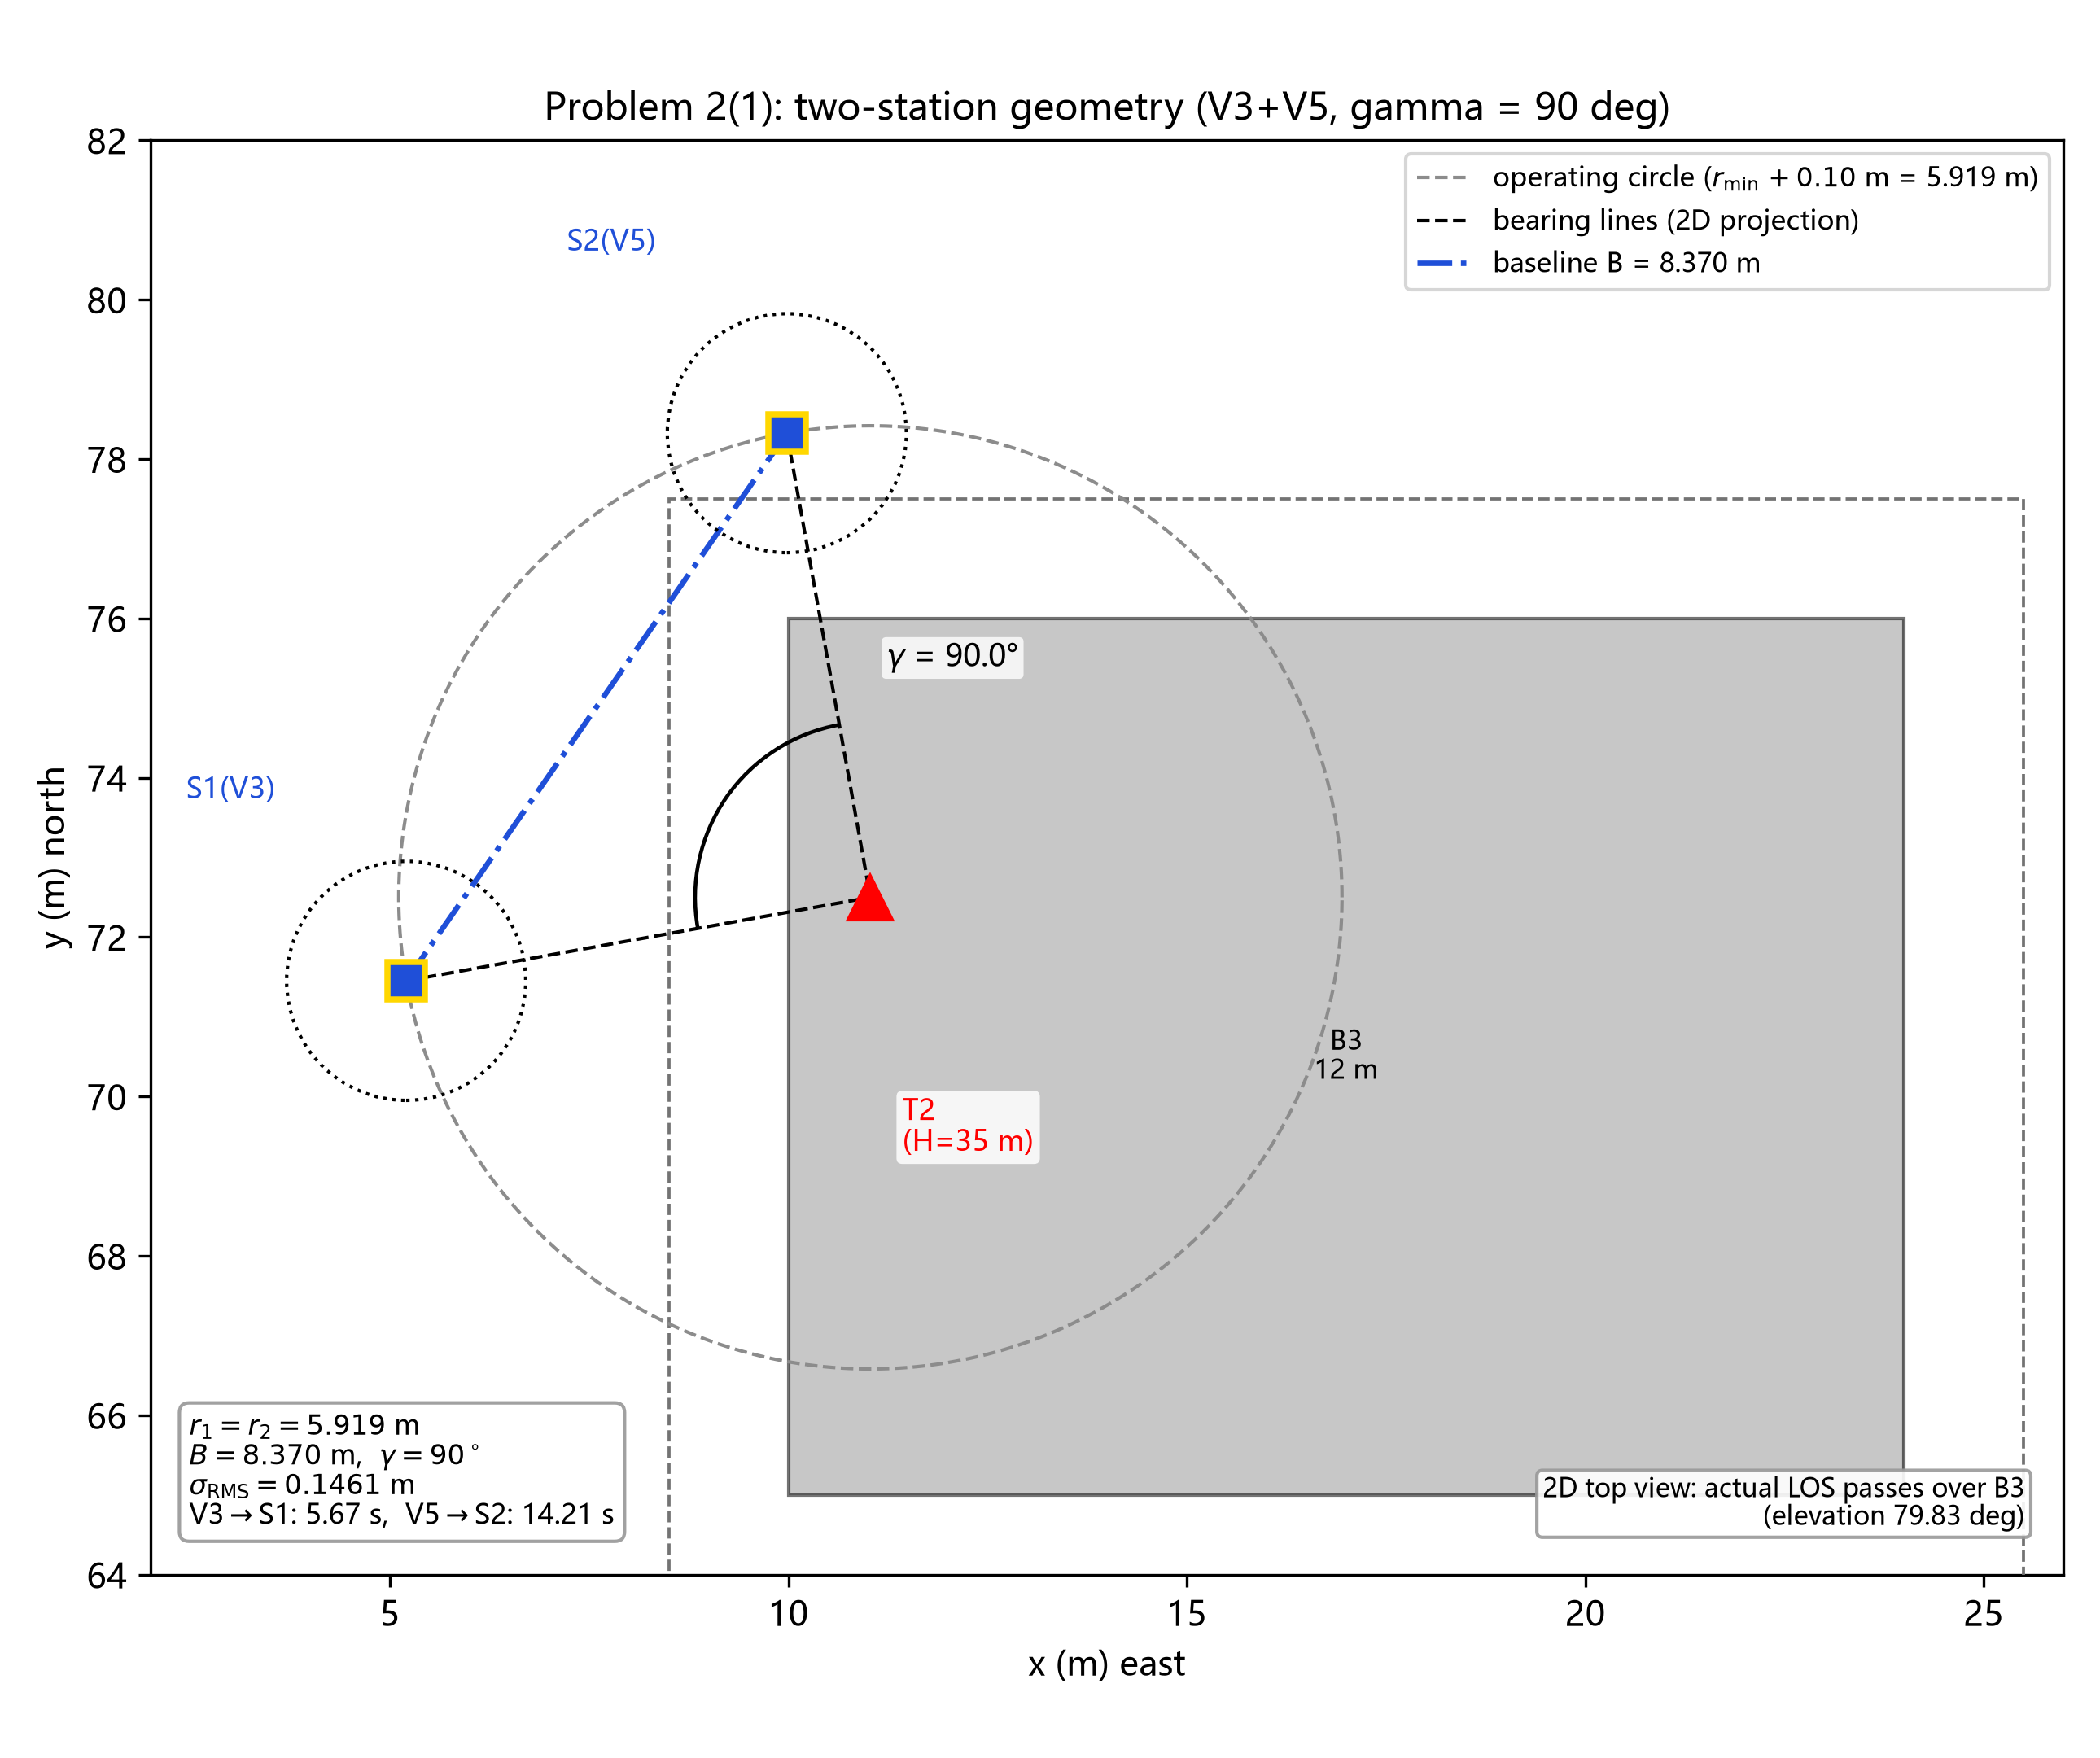
\includegraphics[width=0.6\textwidth]{fig_q2_1_geometry.png}
\caption{Margin-compliant two-station geometry for T2 (V3+V5, $\gamma=90^\circ$,
$r=r_{80}+0.10\,\mathrm{m}$): both stations sit outside the $1.5$-m vehicle buffer
(dashed) with the Assumption-7 margins built in; the horizontal projections of the
sightlines pass over $B_3$ (the actual LOS clears the roof at elevation
$79.83^\circ$, minimum prism distance $0.55\,\mathrm{m}$).}
\label{fig:q2geom}
\end{figure}

The conditional covariance $C$ is \emph{isotropic} ($\operatorname{cond}C=1.000$,
circular $1\sigma$ ellipse of radius $0.1033$ m): at $\gamma=90^\circ$ with equal
distances the two bearing constraints are orthogonal---precisely the geometric meaning
of the bound. The isotropic Gaussian also fixes the operational metric: the radial
error is Rayleigh with median $\mathrm{CEP}_{50}=\sigma_{1D}\sqrt{2\ln2}=0.1216\,\mathrm{m}$
---half of all fixes land within $12$ cm. Both deployed stations carry the declared
margins: elevations $79.83^\circ$ ($0.17^\circ$ below the limit), clearances
$3.30/0.83\,\mathrm{m}$ beyond the buffer, and LOS minimum distances
$2.99/0.55\,\mathrm{m}$ from the nearest prism---the insurance recommended by the
degeneracy discussion is built into the reported deployment.

\textbf{Degenerate configurations.} Equation~\eqref{eq:rmse} quantifies the two
degeneracies the problem asks about. As $\gamma\to0^\circ$ or $180^\circ$,
$\mathrm{RMSE}\propto1/\sin\gamma$ diverges: the two sightlines become parallel, the
position along the baseline direction is unconstrained, $\operatorname{cond}C\to\infty$
and the error ellipse degenerates into a strip (Fig.~\ref{fig:q2gamma}a). The adopted
mitigation is an azimuth guard $\gamma\ge1^\circ$ (hard feasibility) plus an operating
recommendation of $30^\circ\le\gamma\le150^\circ$ read off the sweep. Stations at
region-boundary tangency are handled by the closed-set convention; a margin of
$\delta$ m costs at most $O(\delta)$ in $d_i$. Concretely, the \emph{adopted}
$0.10$-m radial offset keeps $\gamma=90^\circ$, buys $0.17^\circ$ of elevation slack
and $0.83$--$3.30\,\mathrm{m}$ of clearance beyond the buffer, and costs $1.73\%$
RMSE ($0.1461$ vs $0.14362\,\mathrm{m}$)---cheap insurance, built into the reported
deployment rather than left as advice (Section~\ref{sec:sens}).

\begin{figure}[!htb]\centering
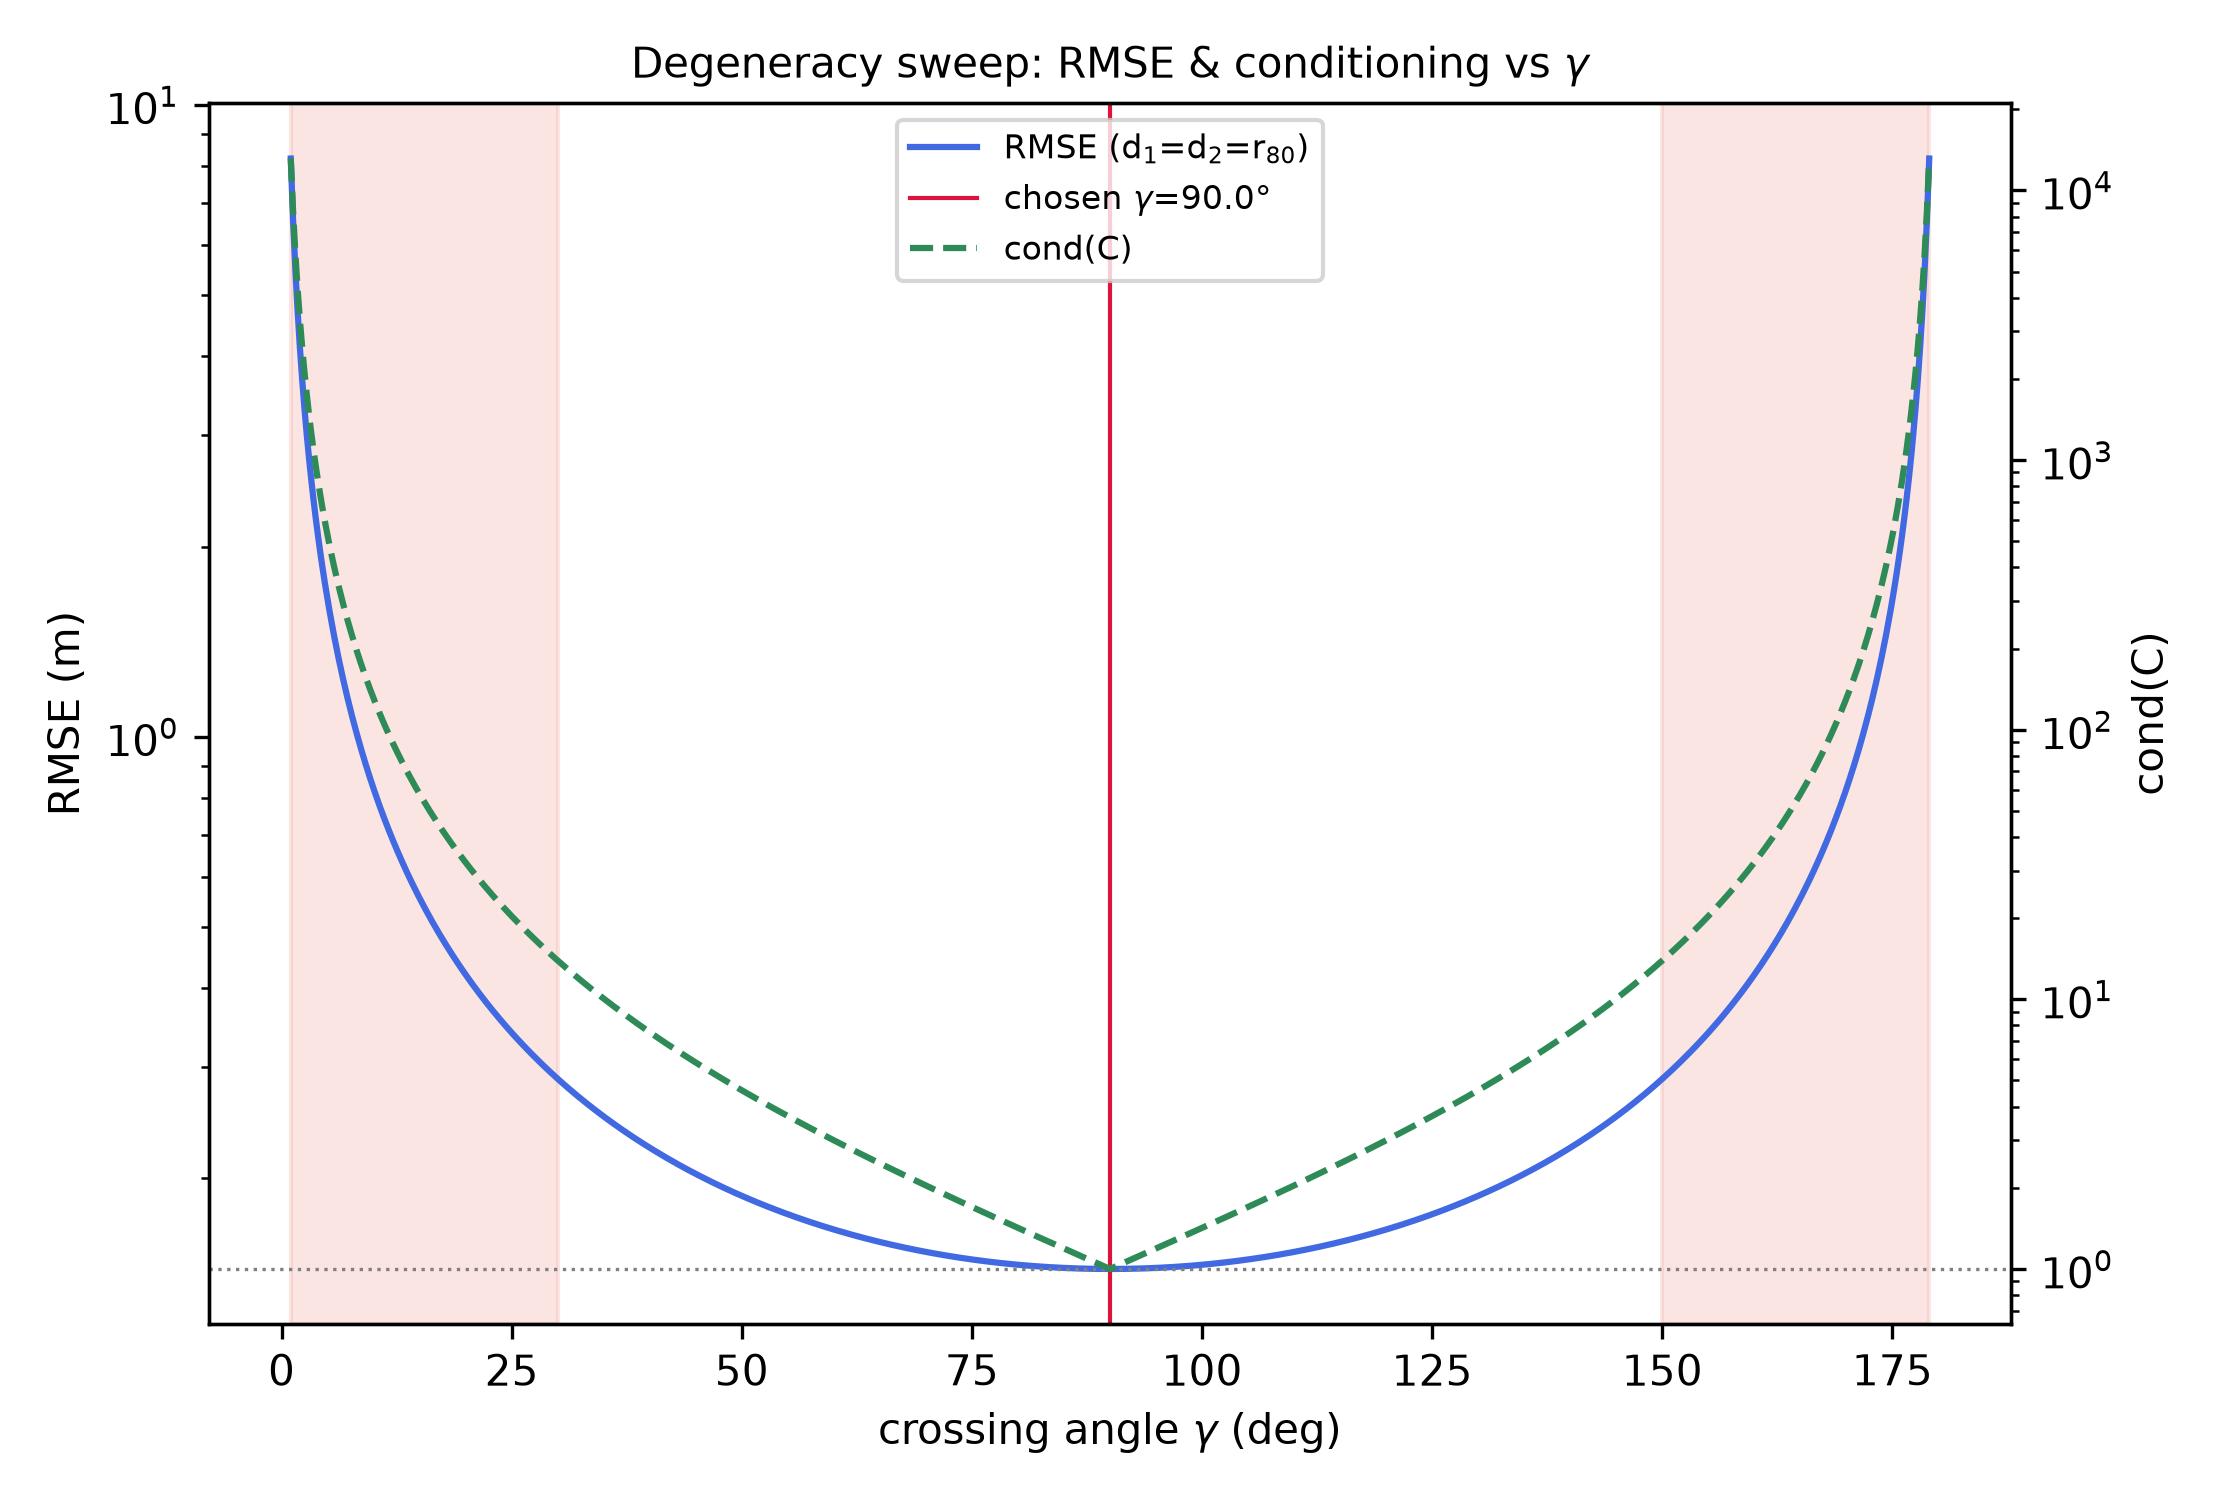
\includegraphics[width=0.46\textwidth]{fig_q2_1_gamma_degeneracy.png}\hfill
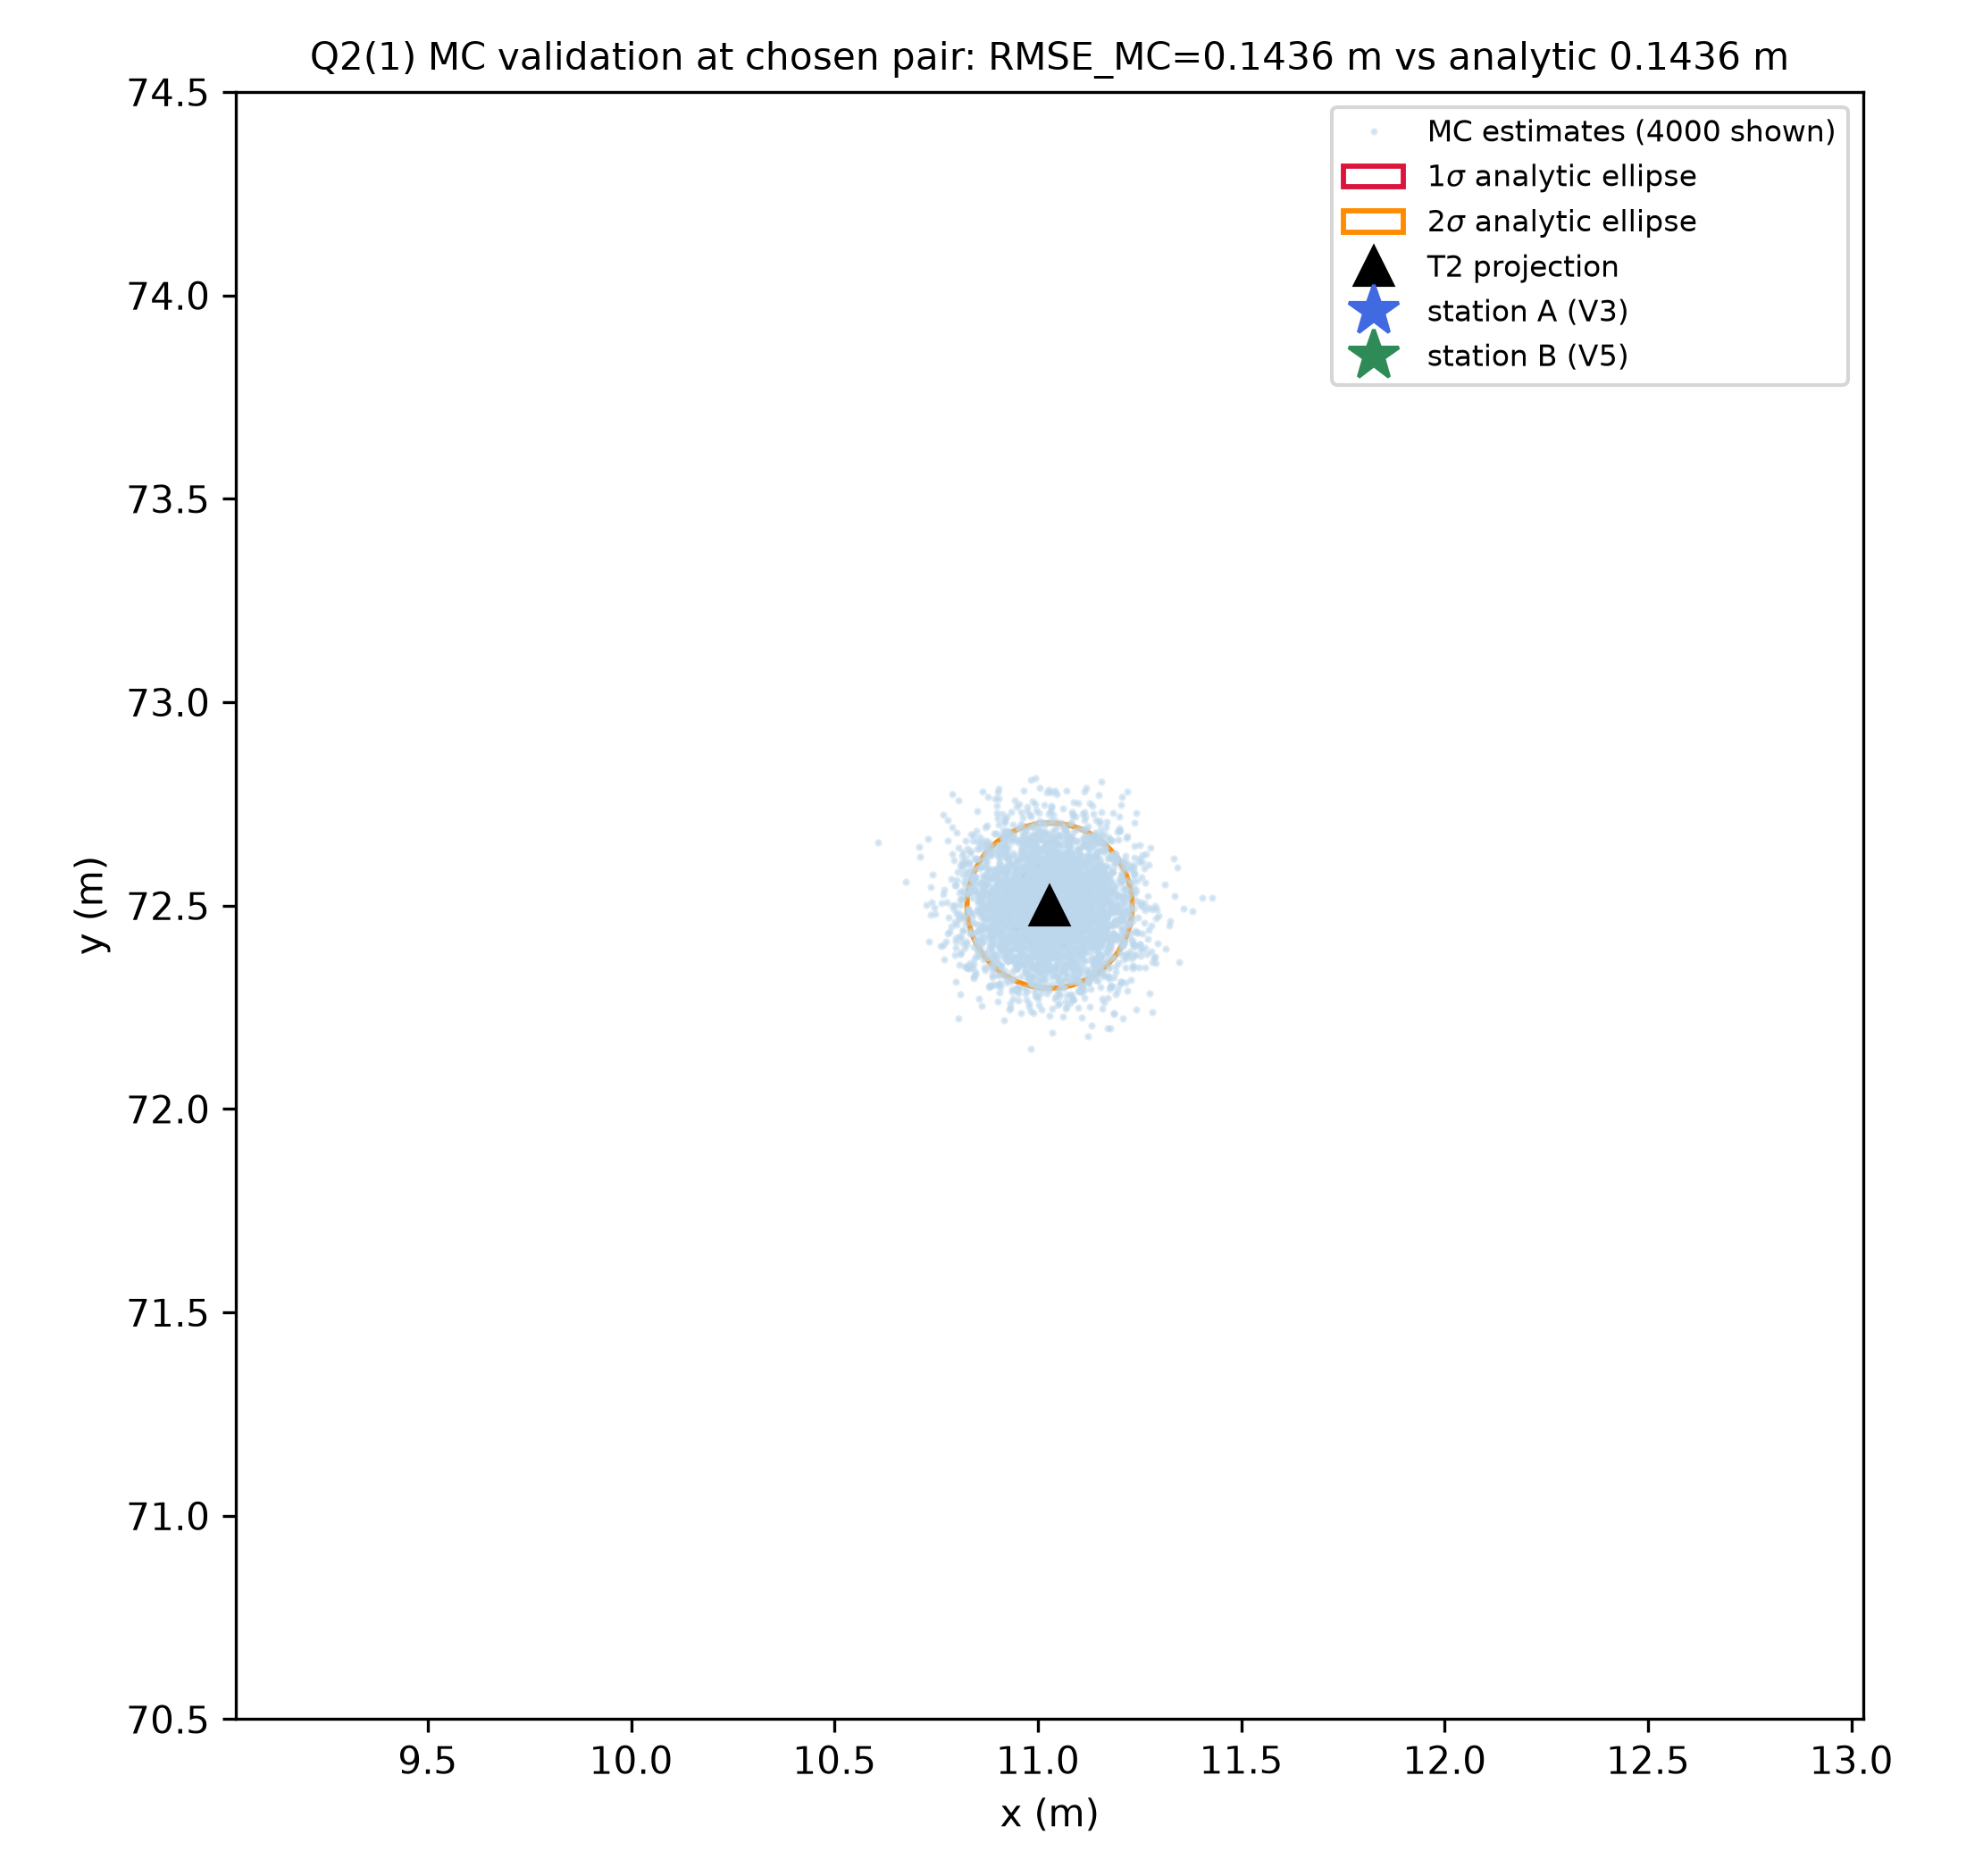
\includegraphics[width=0.46\textwidth]{fig_q2_1_mc_validation.png}
\caption{(a) Degeneracy sweep: RMSE ($\propto1/\sin\gamma$) and $\operatorname{cond}C$
explode as the crossing angle approaches $0^\circ$ or $180^\circ$; the flat band around
$90^\circ$ is operationally safe. (b) Monte Carlo validation ($2\times10^{5}$ samples):
the empirical error scatter (round red) is isotropic with empirical RMSE $0.14363$ m,
matching the analytic covariance ellipse of Eq.~\eqref{eq:fisher} (blue).}
\label{fig:q2gamma}
\end{figure}

\subsubsection{Validation}

A Monte Carlo experiment with $2\times10^{5}$ samples (sampling the two bearing errors,
intersecting the two bearing lines exactly) at the bound geometry yields empirical
RMSE $=0.14363\,\mathrm{m}$ against the analytic $0.14362\,\mathrm{m}$---relative
deviation $0.0\%$ (Fig.~\ref{fig:q2gamma}b); the estimate's Monte-Carlo standard
error, $\mathrm{RMSE}/\sqrt{2N}=2.3\times10^{-4}\,\mathrm{m}$ ($0.16\%$), bounds the
deviation to within one standard error, and the experiment repeats unchanged at the
deployed margin-compliant geometry (all distances scale by $+1.73\%$). The 30-s
travel feasibility of both deployed stations was re-checked on the visibility graph
($17.00$ m and $42.62$ m, well within $90$ m), both stations were re-verified inside
$\mathcal{F}_{T_2}$ by the Q1 solver with the Assumption-7 margins, and the LOS
minimum prism distances ($2.99/0.55\,\mathrm{m}$) certify clearance. Finally,
because $C\propto\sigma_b^2$, re-running the optimization with
$\sigma_b\in\{0.5^\circ,1^\circ,2^\circ\}$ rescales every pair's RMSE proportionally
($0.07301/0.14609/0.29219\,\mathrm{m}$ at the chosen pair) and leaves the argmin unchanged: the
station-pair selection is structurally independent of the bearing-error magnitude.
\emph{Conclusion: the analytic model and the empirical estimator agree to within
Monte Carlo noise, the selected pair is optimal for every $\sigma_b$, and the
deployed margins are verified rather than assumed.}

\subsection{Question 2(2): Vehicle Reuse and Min--Max Scheduling}\label{sec:q22}

\subsubsection{Model}

Three alerts and six task slots with five vehicles force at least one vehicle to serve
two alerts. A \emph{structure} fixes the discrete decisions: the doubling vehicle
$k$, its ordered alert pair, the partner of the doubled vehicle on its first alert, the
partner on its second alert, and the two vehicles of the remaining alert. Within the
single-doubler family (all five vehicles used, exactly one doubles---Assumption~5) the
count is $5\times3\times2\times4!/2=360$; we declare this family as the search scope and
report optimality evidence relative to it. Each alert must be served by two
\emph{different} vehicles from stations inside its observable region, with the azimuth
guard $\gamma\ge1^\circ$ between the two sightlines.

Given a structure and stations, the event-timeline simulator propagates each vehicle's
sequence: driving at $3\,\mathrm{m}/\mathrm{s}$ along obstacle-avoiding shortest paths
(computed by Dijkstra's algorithm on a corner visibility graph
\cite{dijkstra1959,cormen2009}),
slewing $\tau_{slew}=\max(|\Delta\mathrm{pan}|,|\Delta\mathrm{tilt}|)/30^\circ\mathrm{/s}$
from east--level, the joint observation of alert $a$ starting at
\begin{equation}\label{eq:joint}
t^{start}_a=\max\bigl(\,\text{readiness of vehicle 1},\;\text{readiness of vehicle 2}\,\bigr),
\end{equation}
lasting $5\,\mathrm{s}$, followed by a reset back to east--level (zero if already there);
travel gimbal is locked east. The objective is the min--max epigraph---the standard
makespan form of bottleneck scheduling \cite{pinedo2023,boyd2004}---
\begin{equation}\label{eq:minmax}
\min_{\text{structure},\;\text{stations}}\; t^{*}\quad
\text{s.t.}\quad t^{start}_a\le t^{*}\ \ \forall a\in\{T_1,T_2,T_3\},
\end{equation}
with all alert starts evaluated by one and the same simulator (which Q4 later reuses, so
the Q4 baseline is bit-compatible).

\subsubsection{Algorithm}

Two stages. \textbf{Stage A (screening):} for each alert, candidate stations are the
grid-feasible cells (T1: 776, T2: 623, T3: 843 cells) ranked by vehicle travel time;
all 360 structures are evaluated with a greedy station choice per alert (minimax over
the two partners' travel times, azimuth guard enforced), yielding feasible timelines and
their $t^{*}$. \textbf{Stage B (refinement):} the top structures are re-optimized by
best response---each alert's station pair is re-chosen, holding the others fixed, until
no single-alert rechoice reduces $t^{*}$---a coordinate-descent scheme in the standard
best-response family \cite{nocedal2006}---and the survivors are replayed in the
simulator and audited for route validity. The per-alert earliest-start values on the
candidate set (ignoring resource sharing) provide the valid lower bound
$\max_a\mathrm{LB}_a=3.873\,\mathrm{s}$ for Eq.~\eqref{eq:minmax}.

\textbf{Baseline heuristic (required by the problem).} Defined as: (i) each alert
independently picks the station pair minimizing the larger of the two partners' travel
times (per-alert minimax location); (ii) vehicles are assigned first-come--first-served
in alert order $T_1\to T_2\to T_3$; (iii) the forced doubling vehicle orders its two
alerts by marginal delay, choosing the better of its two sequences. The baseline runs on
the same simulator with the same constraints.

\subsubsection{Results}

\begin{figure}[!htb]\centering
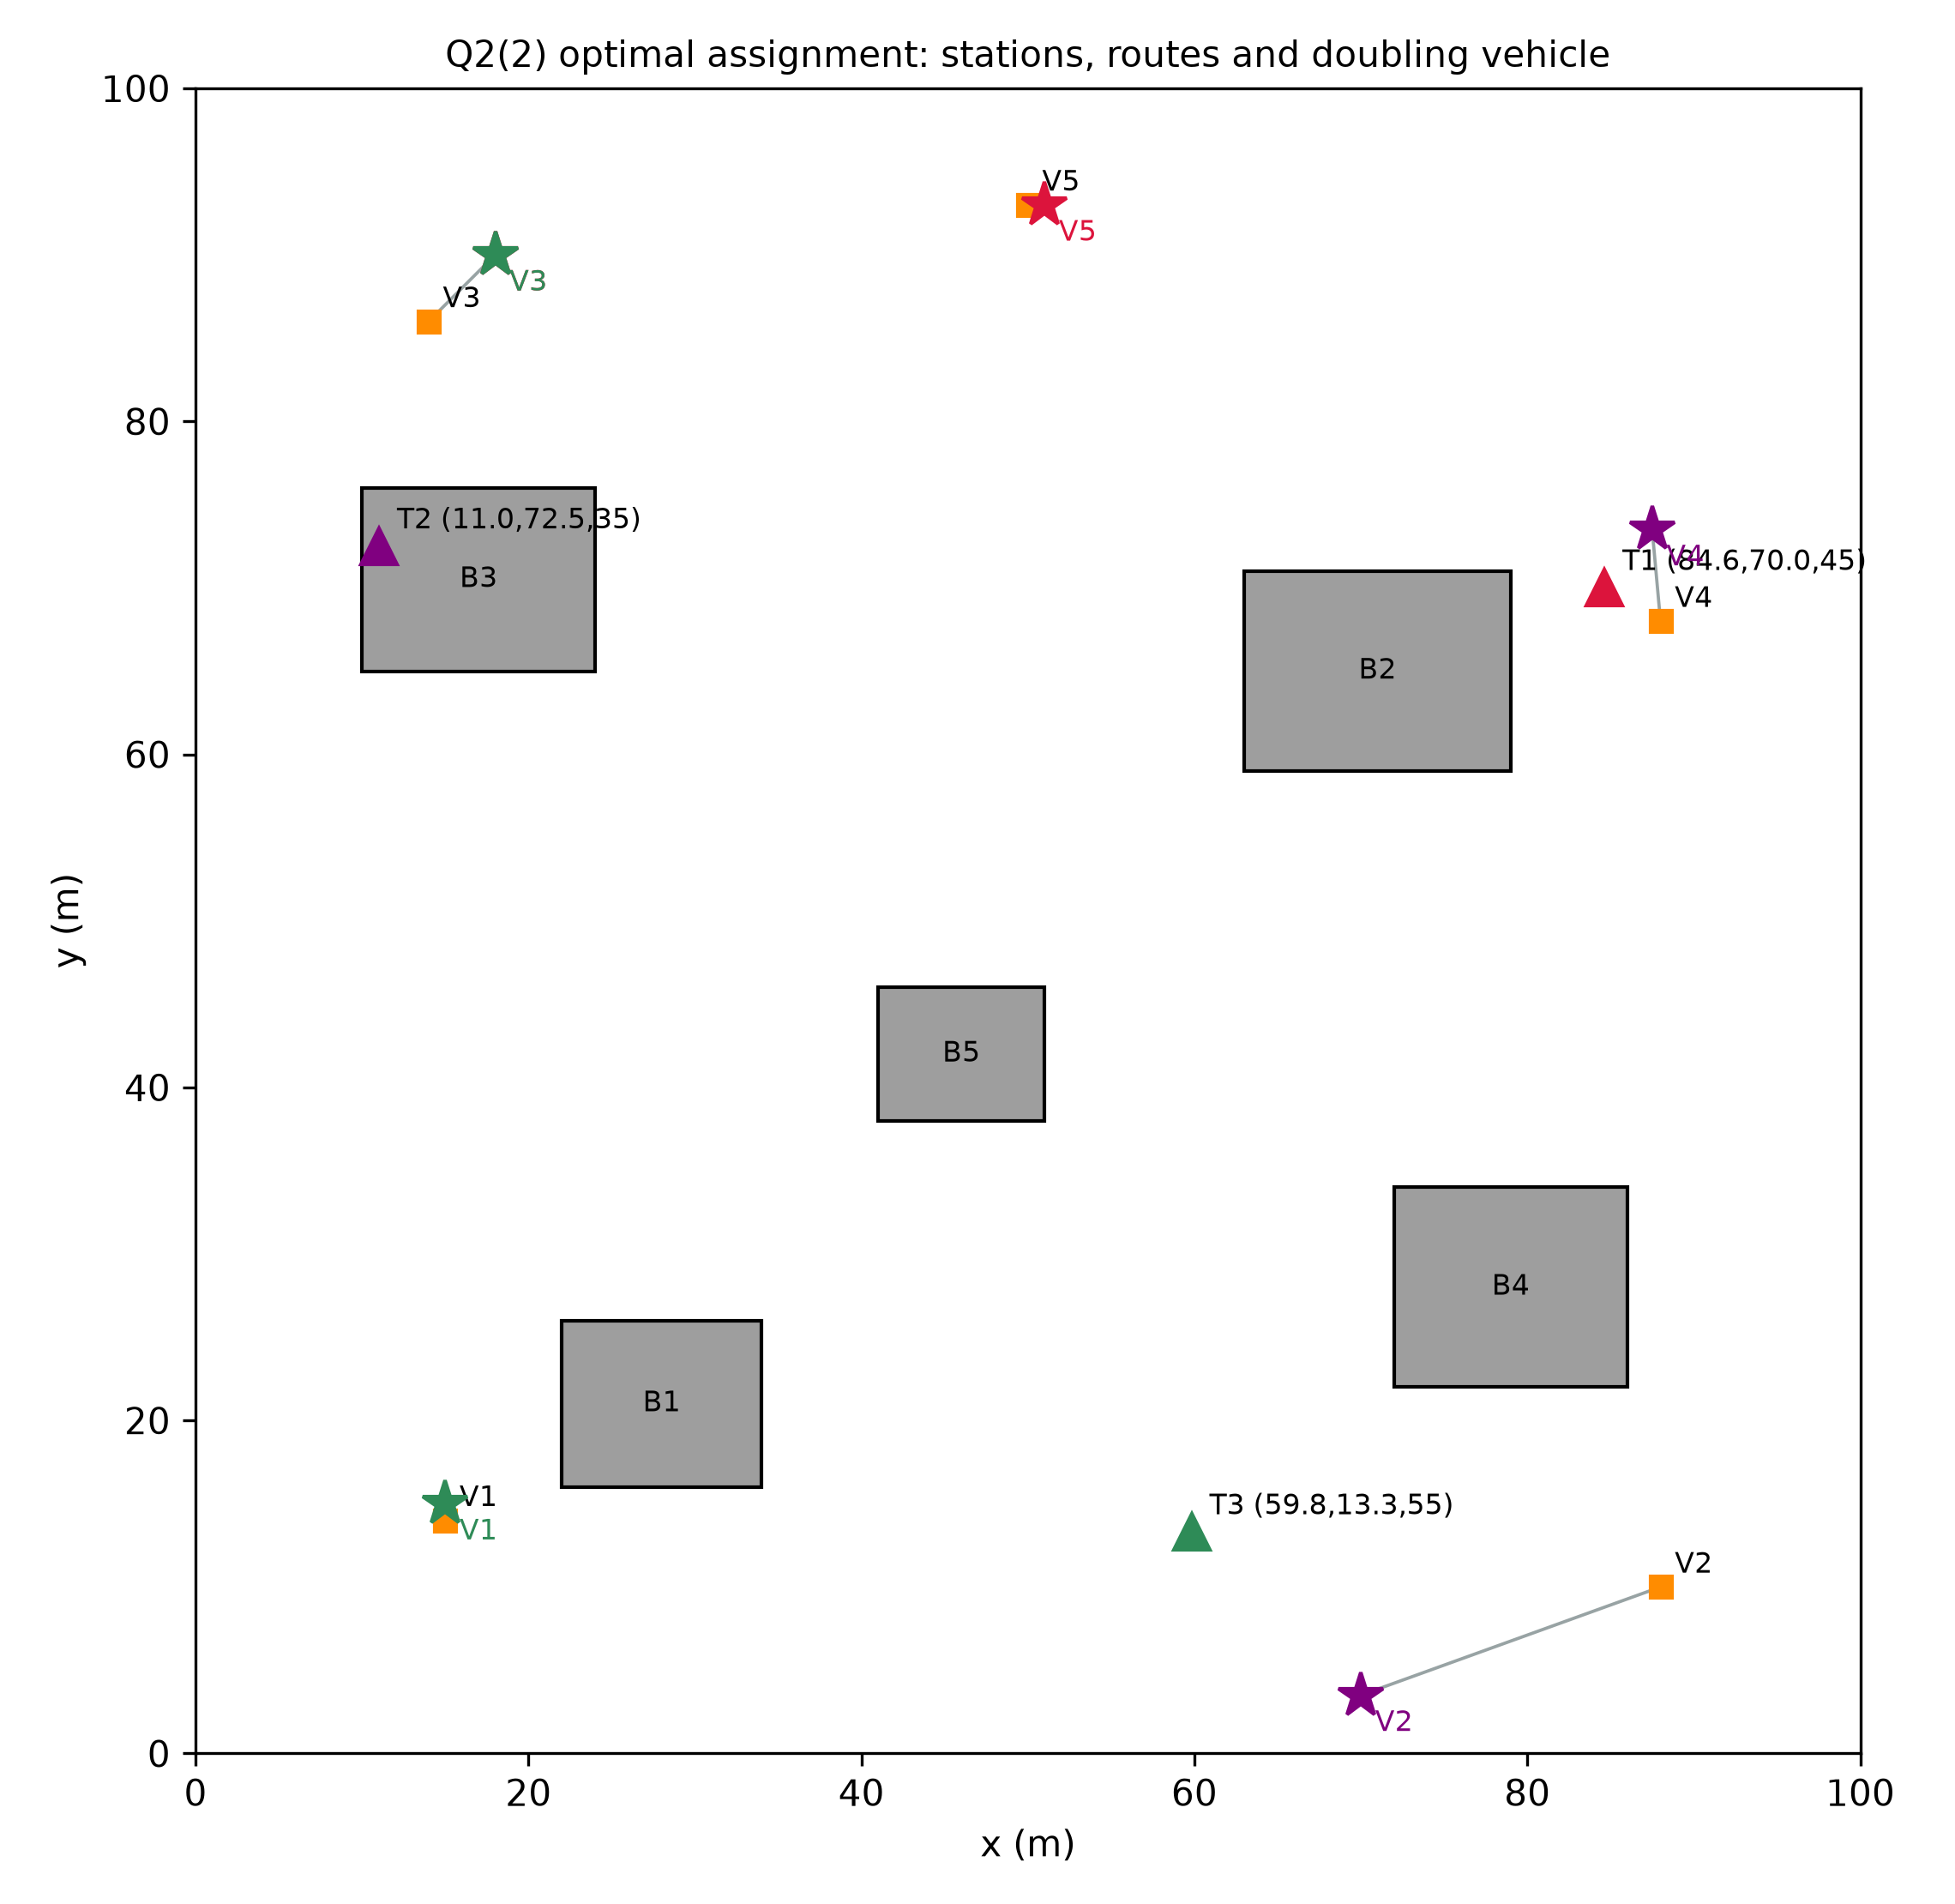
\includegraphics[width=0.42\textwidth]{fig_q2_2_map.png}
\caption{Chosen deployment on the field map: six stations (diamonds) for the three
alerts; V3's two tasks share the single station $(18,90)$, which lies inside both
$\mathcal{F}_{T_1}$ and $\mathcal{F}_{T_3}$, making the second leg zero-travel.}
\label{fig:q2map}
\end{figure}

The optimum found is $t^{*}=11.046\,\mathrm{s}$ with structure ``V3 doubles
$T_1\!\to\!T_3$; V5 partners on $T_1$; V1 partners on $T_3$; V2+V4 serve $T_2$''
(Fig.~\ref{fig:q2map}). Its engine is the shared station $(18,90)$: V3 arrives once,
observes T1 ($2.943$--$7.943\,\mathrm{s}$), resets, and slews in place to T3's bearing
($9.000$--$11.046\,\mathrm{s}$) with \emph{zero} travel---eliminating the round trip that
kills every naive double-task plan. The azimuth-continuous second leg
($343.29^\circ\to298.61^\circ$) also keeps the slew short ($2.046\,\mathrm{s}$).

\begin{table}[!htb]\centering\small
\caption{Per-vehicle event timeline of the chosen schedule (times in s; ``wait'' merges
into obs start where absent).}
\label{tab:q22timeline}
\begin{tabular}{lcccccc}
\toprule
Vehicle--Alert & depart & arrive & ready & obs start & obs end & reset end \\
\midrule
V1--T3 & 0.000 & 0.333 & 1.992 & 11.046 & 16.046 & 17.705 \\
V2--T2 & 0.000 & 6.379 & 10.730 & 10.730 & 15.730 & 20.080 \\
V3--T1 & 0.000 & 1.886 & 2.943 & 2.943 & 7.943 & 9.000 \\
V3--T3 & 9.000 & 9.000 & 11.046 & 11.046 & 16.046 & 18.093 \\
V4--T2 & 0.000 & 1.841 & 7.816 & 10.730 & 15.730 & 21.705 \\
V5--T1 & 0.000 & 0.333 & 1.885 & 2.943 & 7.943 & 9.494 \\
\bottomrule
\end{tabular}
\end{table}

Table~\ref{tab:q22timeline}, Fig.~\ref{fig:q2map} and Fig.~\ref{fig:q2ganttbase}a give
the full timeline: alert
starts are $t^{start}_{T_1}=2.943$, $t^{start}_{T_2}=10.730$,
$t^{start}_{T_3}=11.046\,\mathrm{s}$; the makespan (last reset) is $21.705\,\mathrm{s}$.
The binding alert is T3, whose start is set by V3's arrival from T1's observation plus
the in-place slew---not by V1, ready at T3 since $1.992\,\mathrm{s}$. The azimuth gaps
are $17.65^\circ$ ($T_1$), $50.23^\circ$ ($T_2$), $59.21^\circ$ ($T_3$): the problem
requires only distinct azimuths and accuracy is not the objective here, so the small
$T_1$ gap is admissible; its effect is noted in Section~\ref{sec:sens}.

\begin{figure}[!htb]\centering
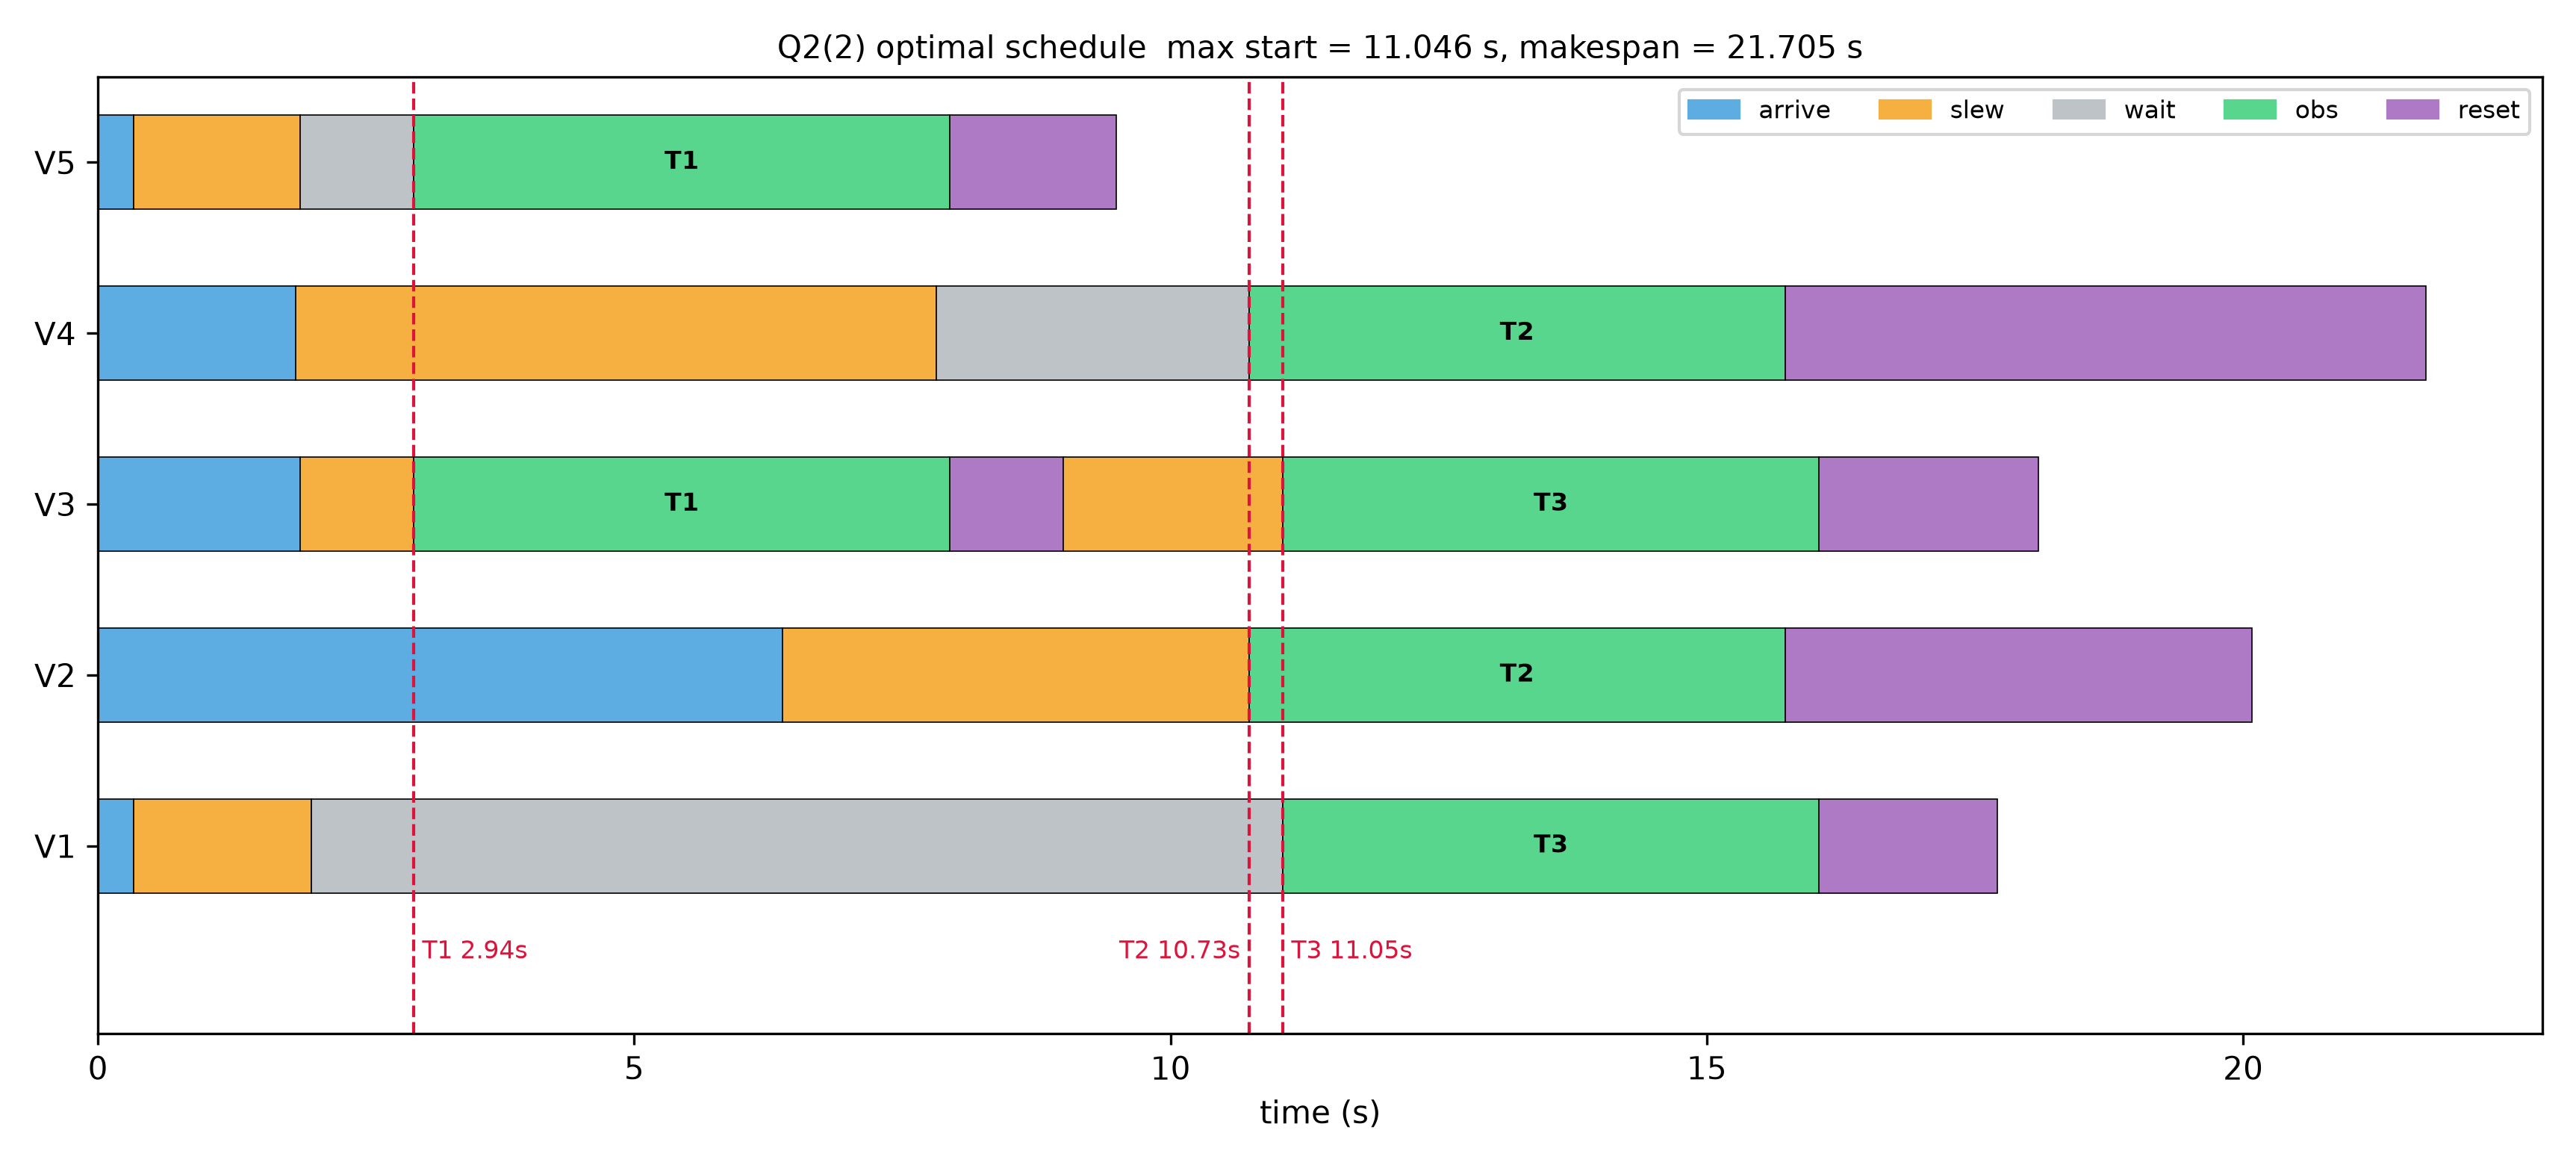
\includegraphics[width=0.49\textwidth]{fig_q2_2_gantt.png}\hfill
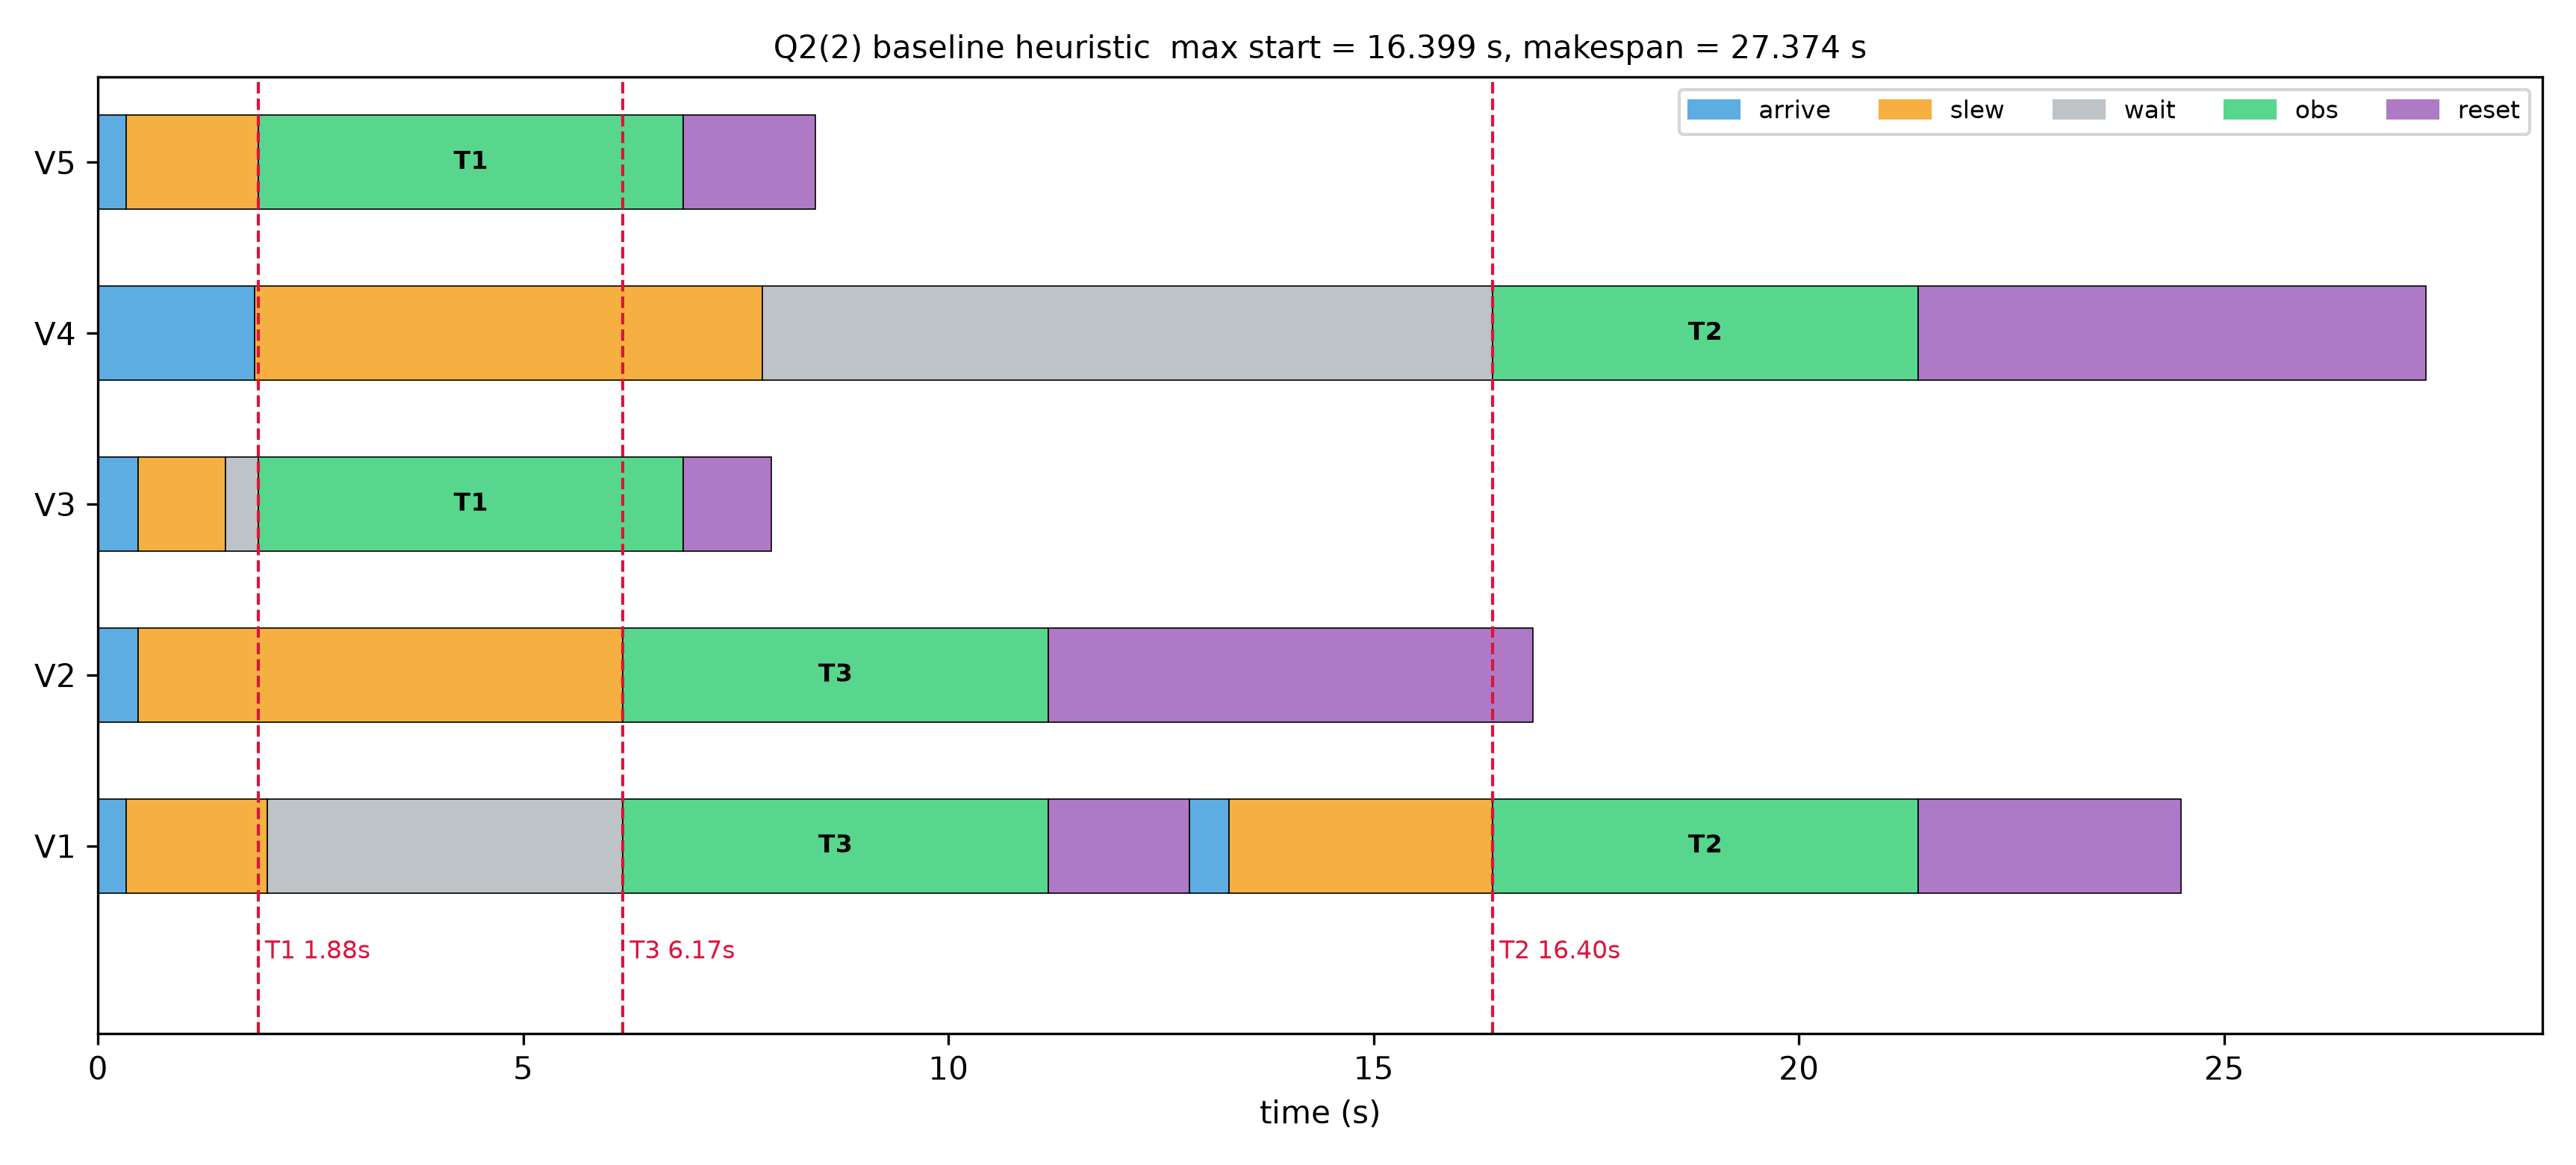
\includegraphics[width=0.49\textwidth]{fig_q2_2_gantt_baseline.png}
\caption{Gantt charts: (a) the chosen schedule; (b) the nearest-assignment baseline,
where V1 doubles $T_3\!\to\!T_2$ and $T_2$---whose independent minimax stations look
attractive locally---starts at $16.399\,\mathrm{s}$, setting the baseline's max.}
\label{fig:q2ganttbase}
\end{figure}

\textbf{Baseline comparison.} The baseline attains $t^{*}=16.399\,\mathrm{s}$: per-alert
starts $T_1$ $1.885$ (equal to its standalone lower bound), $T_3$ $6.172$, $T_2$
$16.399\,\mathrm{s}$. Our schedule improves the max by $5.352\,\mathrm{s}$
($32.6\%$) while individually \emph{losing} on $T_1$ ($-1.058\,\mathrm{s}$) and $T_3$
($-4.875\,\mathrm{s}$)---the signature of the min--max objective, which trades per-alert
excellence for balance. The root cause of the baseline's failure is step (iii): its
doubling vehicle V1 chooses ``$T_3$ first'' by marginal delay, arrives at $T_2$ only
after a full observe--reset--travel cycle, and drags $T_2$ to $16.399\,\mathrm{s}$;
the greedy station choice of step (i), blind to who will double, concentrates the
fastest vehicle (V1) on two nearby alerts and leaves $T_2$ to the slow partner only.
Our structure enumeration sees this interaction explicitly and moves the double task
onto V3 with a shared station instead.

\textbf{Optimality evidence.} No structure among the 360 (with refinement) beats
$11.046\,\mathrm{s}$, and the valid lower bound is $3.873\,\mathrm{s}$ (per-alert earliest
starts ignoring sharing), so the certified gap is $7.17\,\mathrm{s}$; the bound is weak
because it ignores slew and synchronization, and we report it as such rather than
claiming global optimality.

\subsubsection{Validation}

(1) Constraint compliance was re-checked programmatically: every station inside its
observable region, two distinct vehicles per alert, azimuth gaps $\ge1^\circ$, all
routes feasible (V3's legs audited at $5.657$ m and $0$ m with minimum gaps
$\ge10$ m to inflated obstacles). (2) The timeline of Table~\ref{tab:q22timeline} is the
simulator's own output, replayed event-by-event---no manual arithmetic. (3) Parameter
sensitivity ($\pm10\%$) leaves the optimal \emph{structure} unchanged
(Section~\ref{sec:sens}). \emph{Conclusion: the chosen structure is insensitive to
moderate timing-parameter perturbations---no alternative structure overtakes it within
the tested ranges---so the schedule is robust as well as fast.}

\subsection{Question 3: Pointing-Error Propagation and the Maximum Travel}\label{sec:q3}

\subsubsection{Model}

Let the vehicle's estimated position be $\hat P=P+\delta$ with independent per-axis
errors $\delta_x,\delta_y\sim N(0,\sigma_{loc}^2(s))$,
$\sigma_{loc}(s)=0.3+0.02s$ (m), where $s$ is the cumulative travel distance since
departure---the standard additive error decomposition of tracking systems
\cite{barshalom2001}. The target is known exactly. Choose local coordinates with true
sightline vector $T-P=(r,0)$ and $r=40$ m. The commanded azimuth is computed from
$\hat P$, giving the exact position-induced angle and total pointing error
\begin{equation}\label{eq:exactgeom}
\alpha=\operatorname{atan2}(-\delta_y,r-\delta_x),\qquad
\Delta\psi=\operatorname{wrap}_{180}(\alpha+\varepsilon_0+\varepsilon_c),
\end{equation}
where the independent gimbal zero bias and control error are
$\varepsilon_0\sim N(0,0.8^{\circ^2})$ and
$\varepsilon_c\sim N(0,0.6^{\circ^2})$.

\emph{Position-induced term.} The position error projects onto the sightline normal as
$\delta_\perp=\delta\cdot n\sim N(0,\sigma_{loc}^2(s))$ (isotropy), and the small-angle
linearization $\alpha\approx\delta_\perp/r$ gives
\begin{equation}\label{eq:loc}
\Delta\psi_{loc}\approx\frac{\delta_\perp}{r}\cdot\frac{180}{\pi}
\;\Rightarrow\;
\sigma_1(s)=\frac{180}{\pi}\cdot\frac{\sigma_{loc}(s)}{40}
=1.4324\,\sigma_{loc}(s)\ \ [\text{deg}] .
\end{equation}
\emph{Synthesis.} Independent Gaussian sources add in variance:
\begin{equation}\label{eq:tot}
\sigma_{tot}(s)=\sqrt{\sigma_1(s)^{2}+0.8^{2}+0.6^{2}},\qquad
P\bigl(|\Delta\psi|\le5^\circ\bigr)=2\Phi\!\Bigl(\frac{5}{\sigma_{tot}(s)}\Bigr)-1 .
\end{equation}
The wrap of $\Delta\psi$ into $[-180^\circ,180^\circ)$ is irrelevant in the feasible
region (verified below).

\emph{Inverse problem.} The reliability requirement
$P\ge0.95$ is equivalent to $z_{0.975}\,\sigma_{tot}\le5$ with $z_{0.975}=1.959964$,
i.e.\ $\sigma_{tot}\le2.551067^\circ$. Peeling Eq.~\eqref{eq:tot} backwards:
$\sigma_1\le2.346901^\circ$, $\sigma_{loc}\le1.638446\,\mathrm{m}$, and with
$\sigma_{loc}(s)=a+bs$ at $s=80$:
\begin{equation}\label{eq:chain}
s_{\max}=\frac{1.638446-0.3}{0.02}=66.9223\ \mathrm{m},
\qquad
a+80\,b\le1.638446,\quad a,b\ge0 .
\end{equation}
The $(a,b)$ feasible set is the right triangle with vertices $(0,0)$, $(1.6384,0)$,
$(0,0.02048)$, shown in Fig.~\ref{fig:q3ab}. The full-geometry check below tightens its
boundary to $a+80b\le1.636745$.

\begin{figure}[!htb]\centering
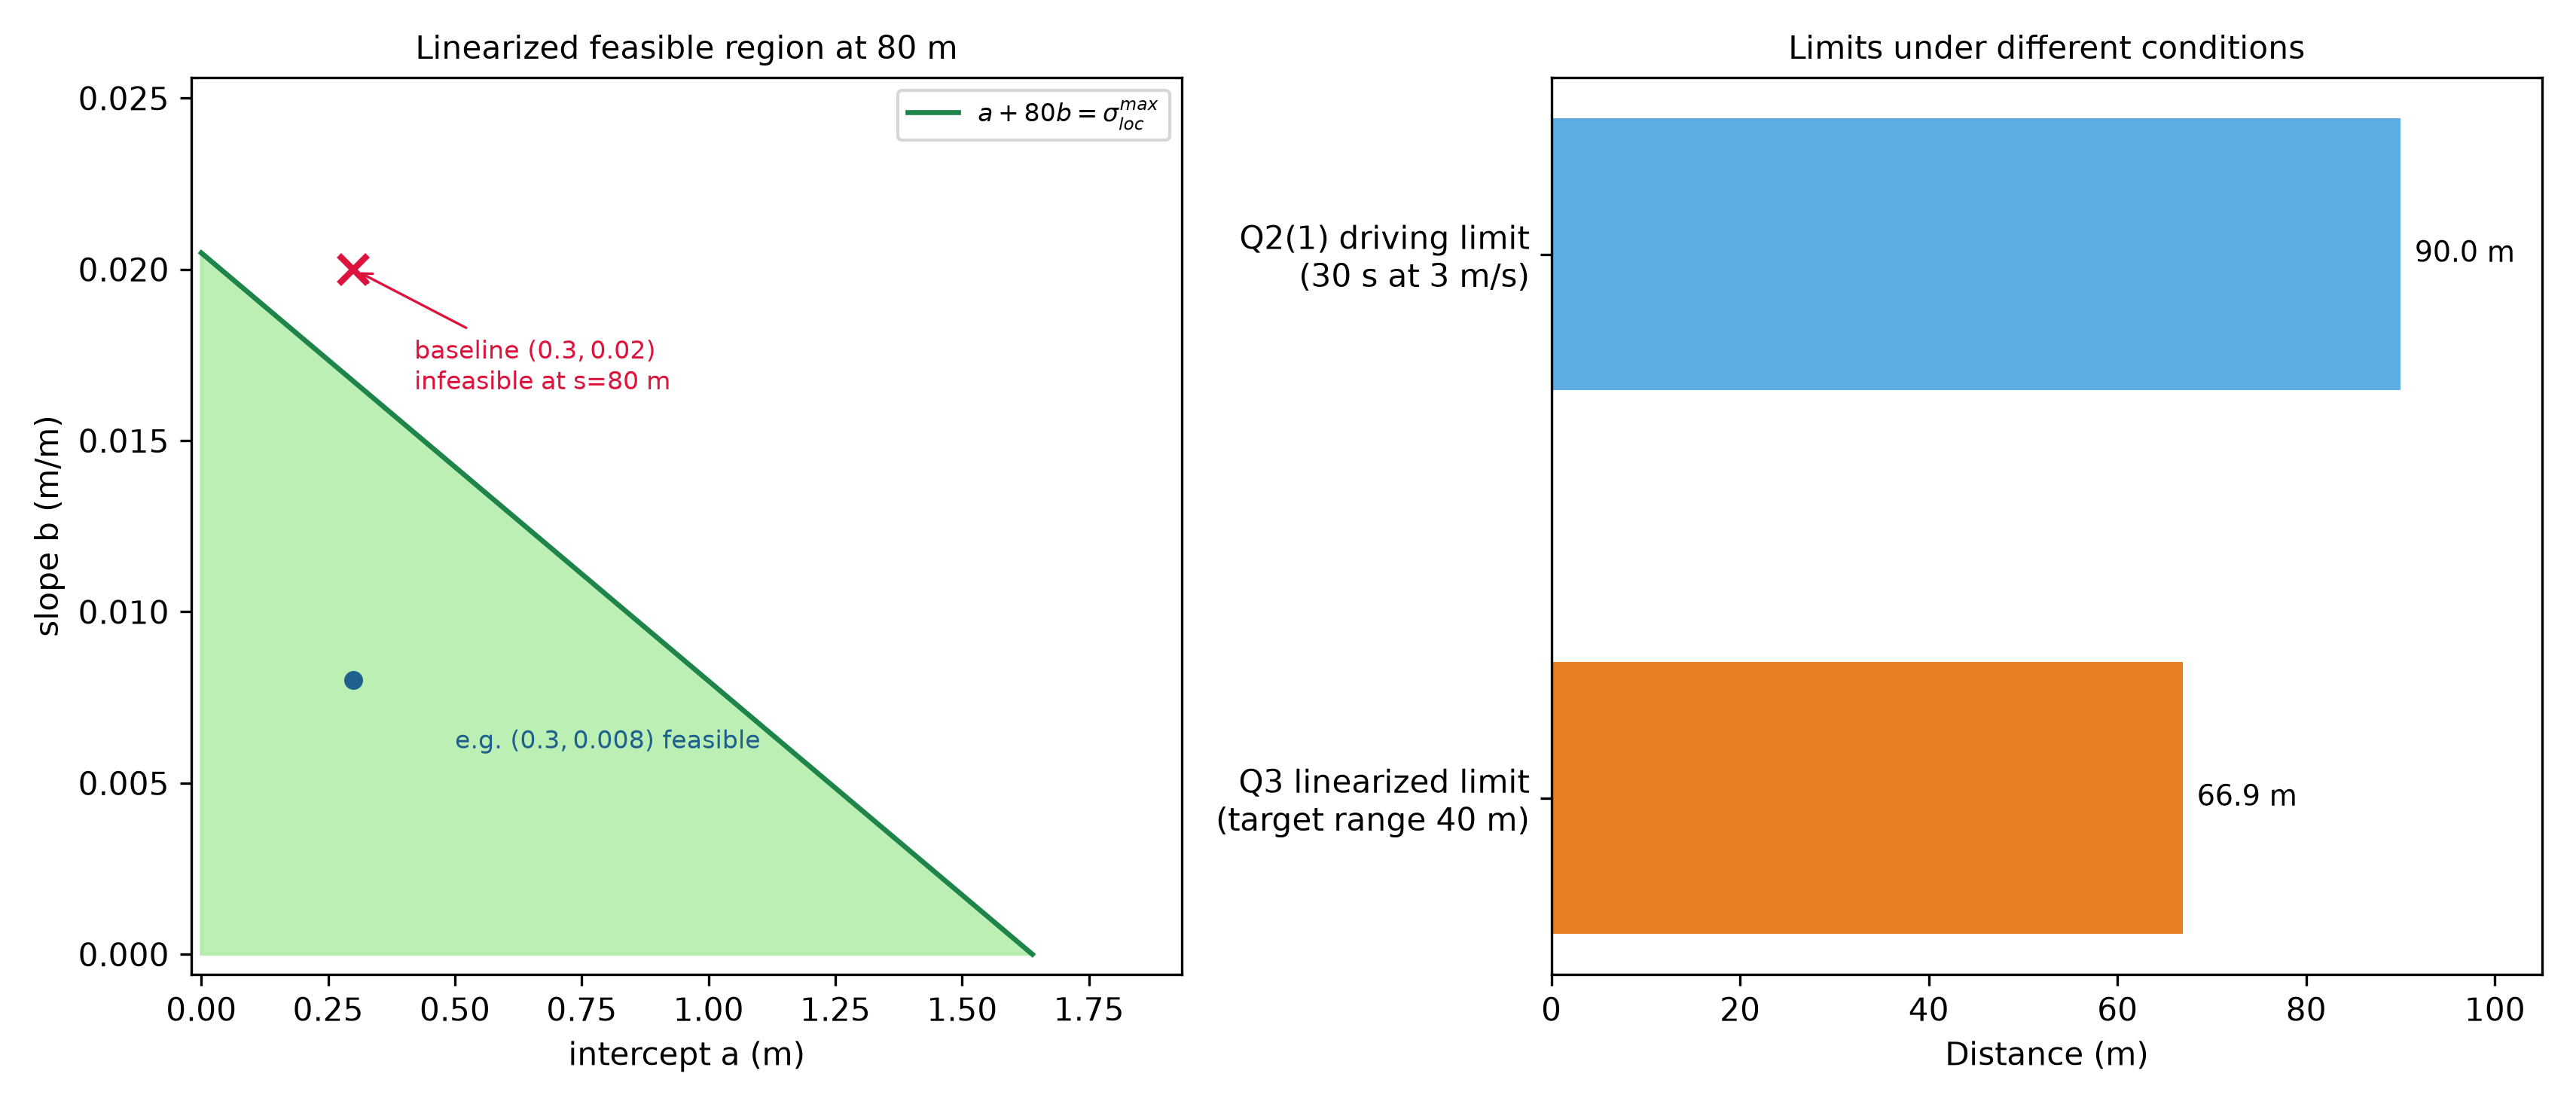
\includegraphics[width=0.39\textwidth]{fig_q3_ab_region.png}
\caption{Feasible region of the error-growth law $(a,b)$ at the 80-m operating point
(shaded): the baseline $(0.3,0.02)$ lies strictly outside---at $80$ m the linearized
pointing reliability would be only $91.54\%$ (full geometry: $91.51\%$).}
\label{fig:q3ab}
\end{figure}

\subsubsection{Justification of the Approximations}

Three approximations enter Eq.~\eqref{eq:loc}--\eqref{eq:tot}.
(i) \emph{Linearization}: arctan nonlinearity and the denominator $r-\delta_x$ have
one-sigma relative scales $0.0559\%$ and $4.0961\%$ at the cap. For $|\alpha|\ge1^\circ$
(avoiding near-zero ratios), the $5\times10^6$-sample diagnostic gives 99th-percentile and
maximum relative errors $10.55\%$ and $20.35\%$; Eq.~\eqref{eq:pexact} below measures
their actual reliability impact.
(ii) \emph{Wrapping}: the linearized tail beyond $180^\circ$ at $80\,\mathrm{m}$ underflows
in double precision, while full \texttt{atan2} and wrap remain in both independent checks.
(iii) \emph{Gaussian synthesis}: exact within the linearized model by independence.

For an approximation-free probability check, let $\lambda(s)=r/\sigma_{loc}(s)$ and
$\sigma_g=\sqrt{0.8^2+0.6^2}=1^\circ$. The exact angle $\alpha$ in
Eq.~\eqref{eq:exactgeom} has density
\begin{equation}\label{eq:angledensity}
f_\lambda(\theta)=\frac{e^{-\lambda^2/2}}{2\pi}
+\frac{\lambda\cos\theta}{\sqrt{2\pi}}\,
e^{-\lambda^2\sin^2\theta/2}\Phi(\lambda\cos\theta),
\qquad -\pi\le\theta\le\pi .
\end{equation}
Convolving this density with the Gaussian gimbal error gives the one-dimensional integral
\begin{equation}\label{eq:pexact}
P_{exact}(s)=\int_{-\pi}^{\pi}f_{\lambda(s)}(\theta)
\left[\Phi\!\left(\frac{5^\circ-\theta_{deg}}{\sigma_g}\right)
-\Phi\!\left(\frac{-5^\circ-\theta_{deg}}{\sigma_g}\right)\right]d\theta,
\quad \theta_{deg}=\frac{180\theta}{\pi},
\end{equation}
which we evaluate by adaptive quadrature, without linearization or sampling error.

\subsubsection{Results and Validation}

\begin{figure}[!htb]\centering
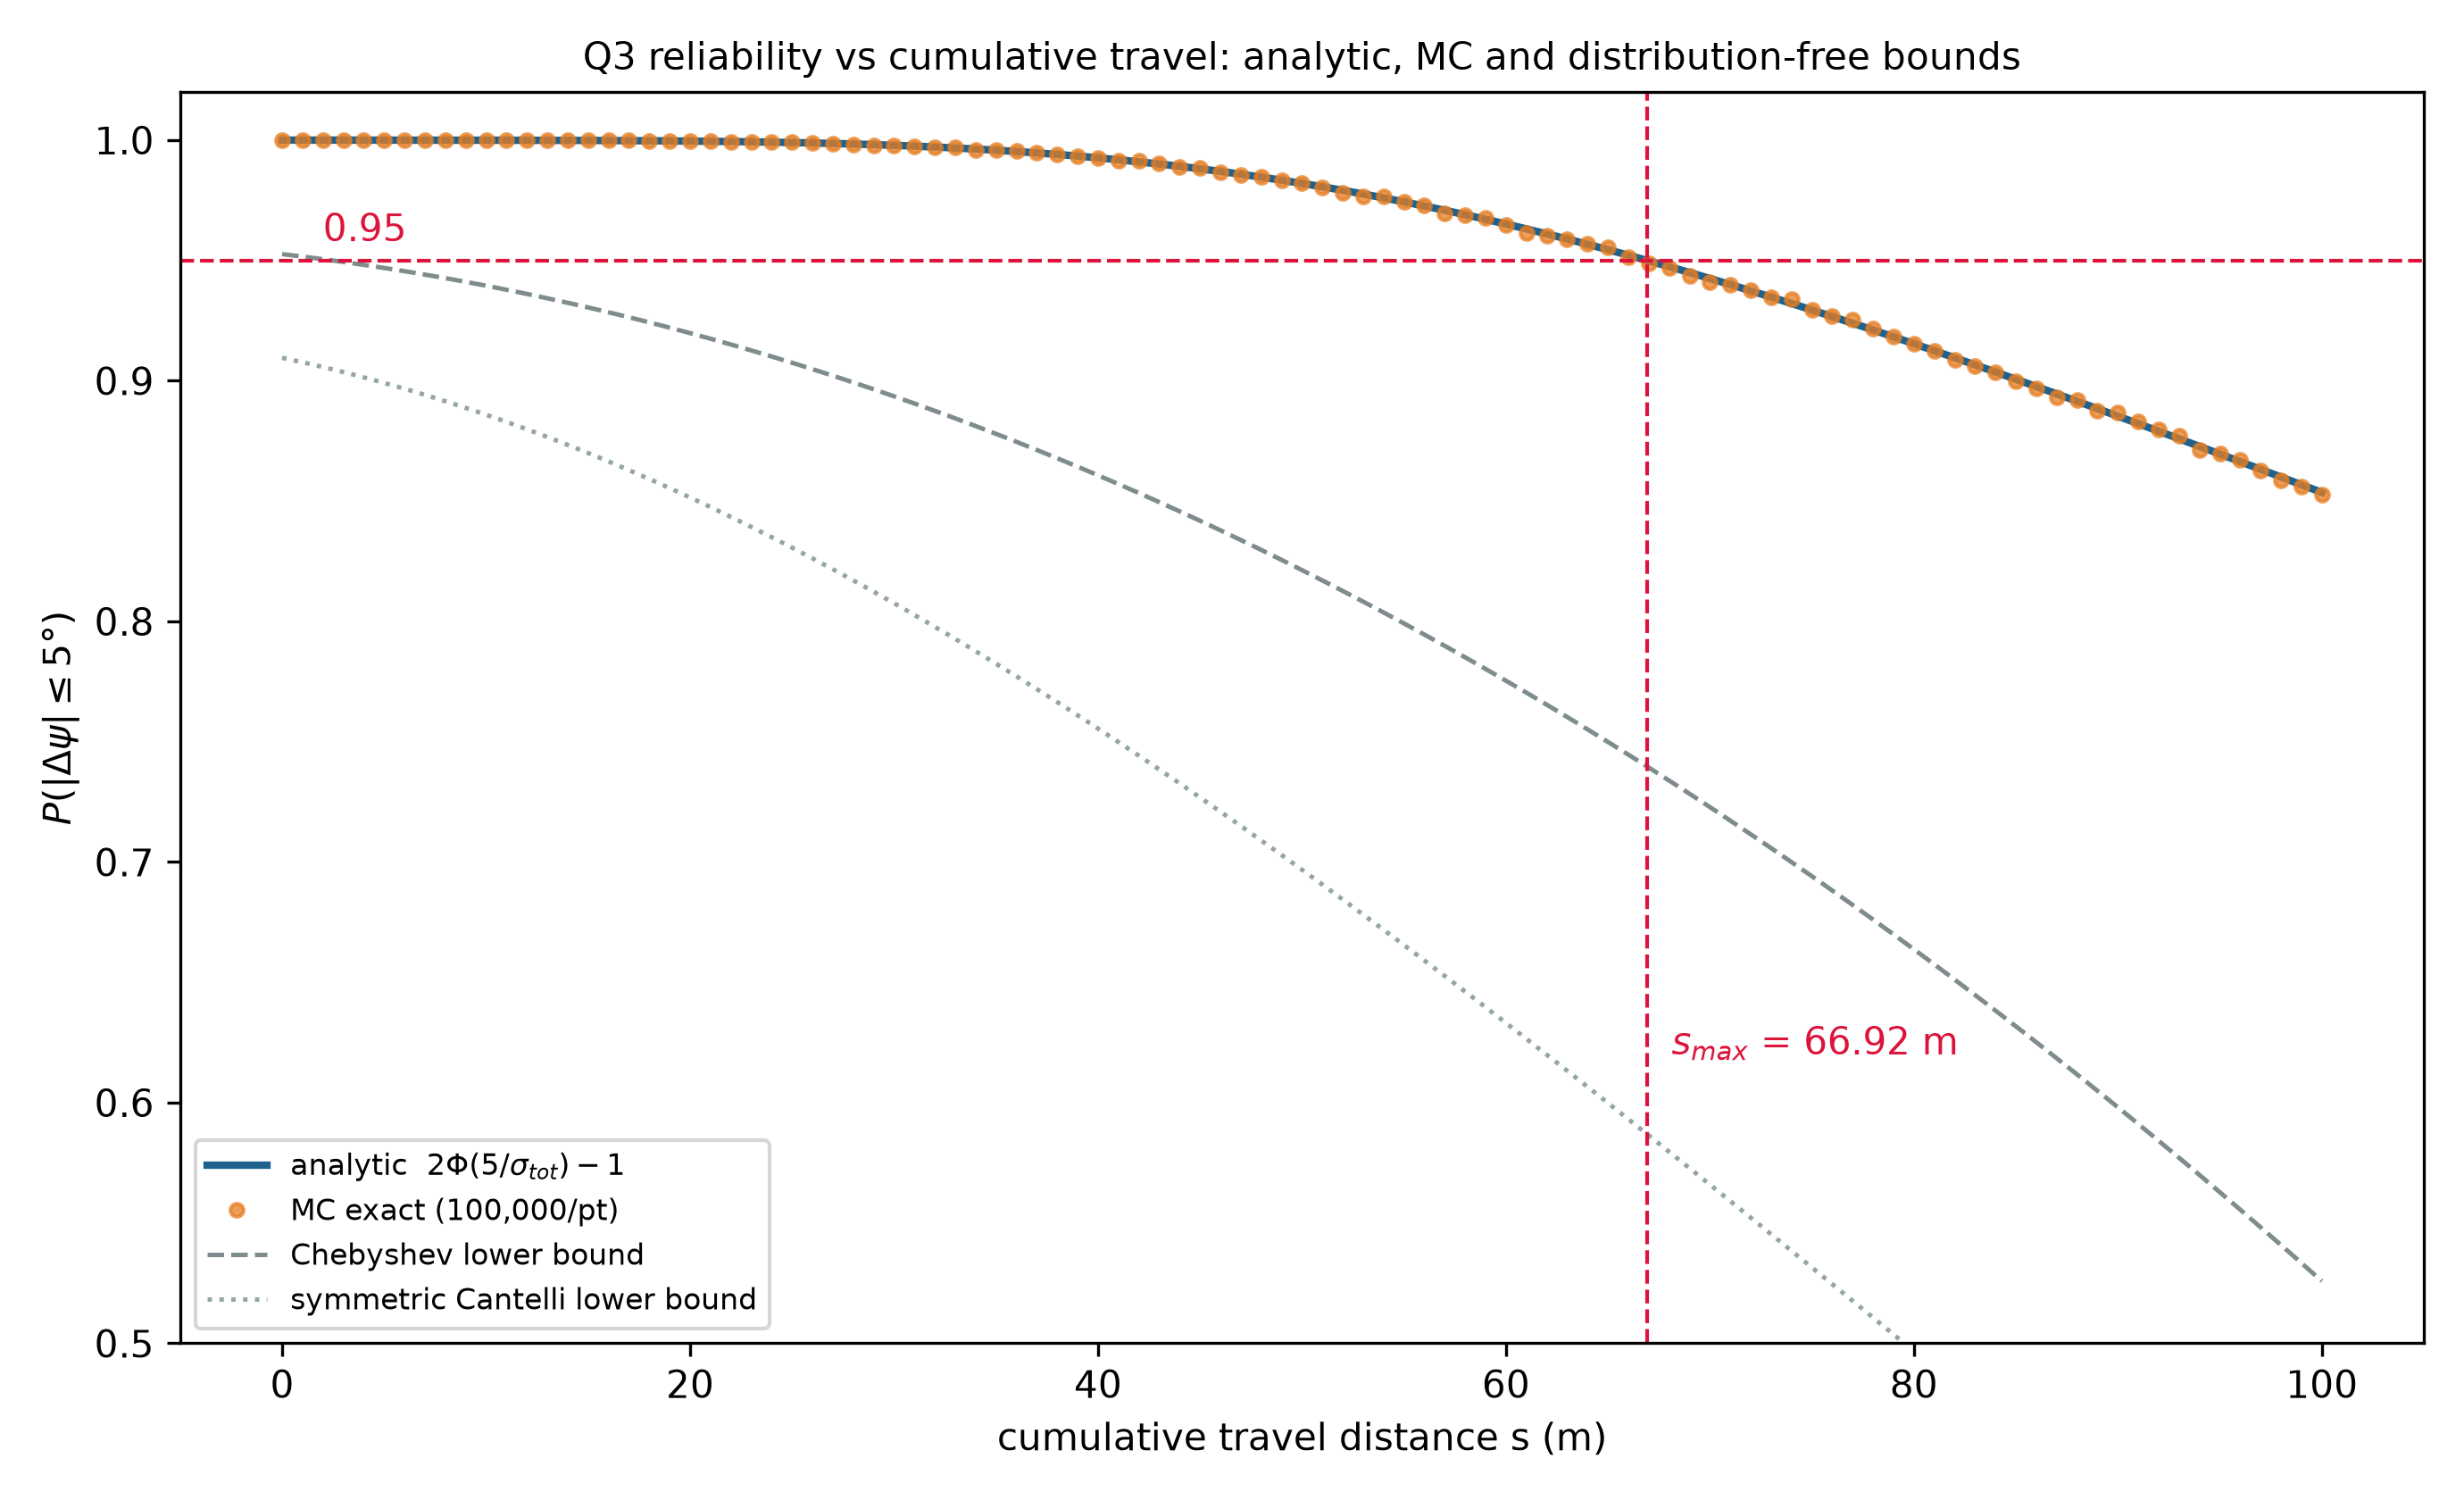
\includegraphics[width=0.39\textwidth]{fig_q3_p_s_curve.png}\hfill
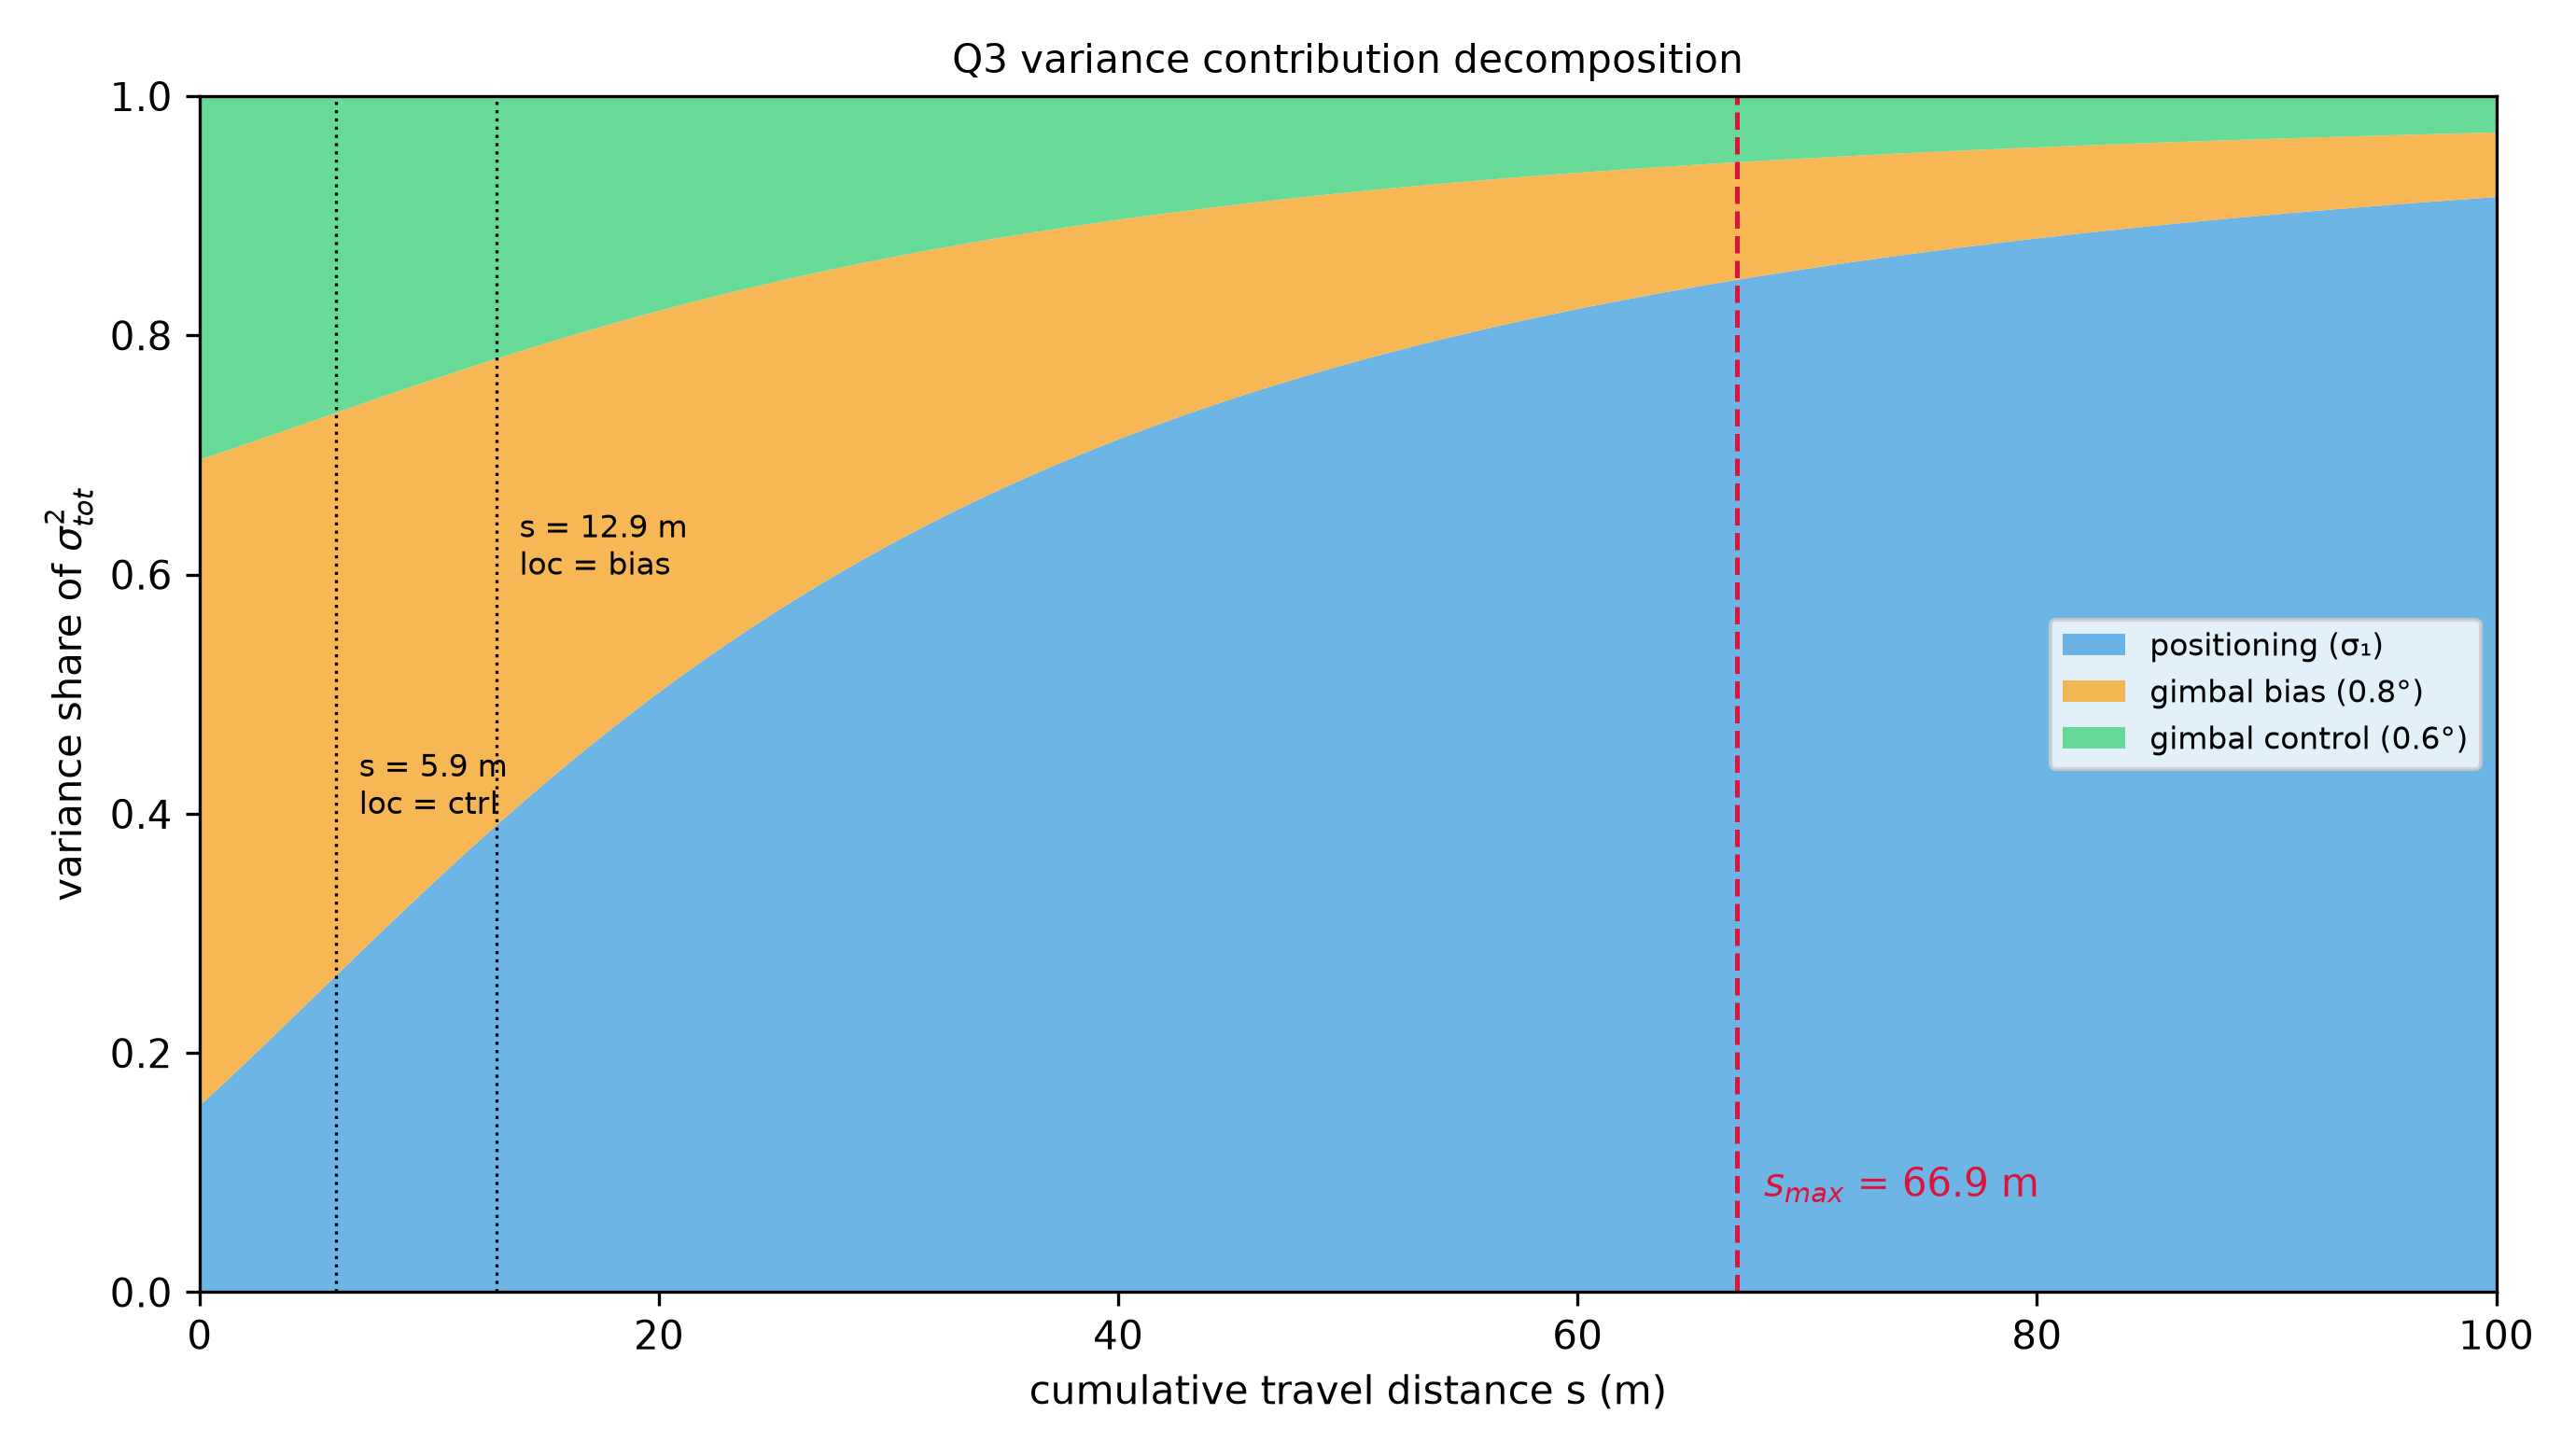
\includegraphics[width=0.39\textwidth]{fig_q3_contribution.png}
\caption{(a) Pointing reliability $P(|\Delta\psi|\le5^\circ)$ versus cumulative travel:
analytic chain (line) and exact-geometry Monte Carlo, $10^{5}$ samples per point, seed
2026 (dots); the dashed rule marks the $95\%$ requirement, crossing at
$s_{\max}=66.92\,\mathrm{m}$. (b) Variance-contribution decomposition along $s$: gimbal
zero bias dominates below $12.93\,\mathrm{m}$ (54.0\% at $s=0$), control error below
$5.94\,\mathrm{m}$; beyond $40\,\mathrm{m}$ the localization term owns $71.3\%$, rising
to $88.1\%$ at $80\,\mathrm{m}$.}
\label{fig:q3ps}
\end{figure}

Over $s\in[0,100]\,\mathrm{m}$, Fig.~\ref{fig:q3ps}a has maximum analytic--Monte Carlo
deviation $0.18$ percentage points; the interpolated Monte Carlo crossing is
$66.56\,\mathrm{m}$, $0.36\,\mathrm{m}$ below the analytic cap. At that cap,
Eq.~\eqref{eq:pexact} gives $P_{exact}=0.9497982$; a $5\times10^6$-sample exact-geometry
simulation gives $0.9498684$, Wilson 95\% CI \cite{wilson1927}
$[0.9496768$, $0.9500593]$. Solving $P_{exact}(s)=0.95$ gives $66.8373\,\mathrm{m}$,
where the same-size simulation gives $0.9500798$, Wilson interval $[0.9498886$,
$0.9502703]$.
Both intervals contain their quadrature targets.

The linearized cap exceeds the exact crossing by $0.0850\,\mathrm{m}$, hence is slightly
\emph{non-conservative}, although the reliability difference is only $0.0202$ percentage
points. We retain $66.9223\,\mathrm{m}$ as the analytic answer, report the full-geometry
bound as $66.8373\,\mathrm{m}$ ($66.84\,\mathrm{m}$), and deploy at $66.83\,\mathrm{m}$
without rounding upward. At $80\,\mathrm{m}$, baseline reliability is $91.5376\%$
(linearization) and $91.5068\%$ (full geometry): an 80-m approach is infeasible.

Chebyshev's distribution-free bound is only $2.45\,\mathrm{m}$; symmetric Cantelli is
infeasible because $\sigma_{tot}^2\le0.641$ is below the fixed gimbal variance $1.0$.
Figure~\ref{fig:q3ps}b gives crossovers at $5.94\,\mathrm{m}$ (control) and
$12.93\,\mathrm{m}$ (bias); localization owns over half the variance beyond
$19.91\,\mathrm{m}$.

\textbf{Deployment insight (feeding Q2/Q4).} The strict $66.83\,\mathrm{m}$ cap binds
before Q2(1)'s 90-m driving budget, so travel must stay below it or tasks must rotate.
All reported schedules comply; Q2(2)'s legs span $0$--$19.1\,\mathrm{m}$.

\subsection{Question 4: Disturbance Rescheduling and Strategy Comparison}\label{sec:q4}

\subsubsection{Event Model and State Capture}

The refined margin-compliant Q2(2) schedule of Section~\ref{sec:q22}
($t_{\mathrm{last}}=10.651\,\mathrm{s}$; alert starts $2.388/7.501/10.651\,\mathrm{s}$)
is the operating baseline. At $t=5\,\mathrm{s}$ a disturbance occurs;
the evaluation window is $[0,60]\,\mathrm{s}$. Three primitive events, used alone or in
combination, generate 86 test scenarios:
\begin{itemize}
\item \textbf{(a) New alert.} $T_4=O+R(\cos\theta,\sin\theta)$, $H=50\,\mathrm{m}$
(same polar convention as $T_1$--$T_3$); $\theta$ swept over
$15^\circ{:}30^\circ{:}345^\circ$, $R\in\{30,40,50\}\,\mathrm{m}$ (36 grid points).
\item \textbf{(b) Vehicle failure.} One of V1--V5 exits the field (non-obstructing);
any alert whose joint observation has \emph{not} started and whose assigned pair
contains the failed vehicle is lost under a no-response policy.
\item \textbf{(c) Communication outage.} Orders issued in $[5,t_{rec}]$ cannot reach
the vehicles, which continue on the original plan; new orders take effect upon
recovery, so the decision epoch is $\tau=t_{rec}$.
\end{itemize}
At the decision epoch $\tau$ the dispatcher captures the true state: alerts whose joint
observation already started are \emph{locked} (non-reschedulable; $T_1$ is always
locked since it started at $2.388\,\mathrm{s}<5\,\mathrm{s}$); vehicles are described
by position, current pan/tilt attitude, and free time; reassigned vehicles travel from
their \emph{current} position. A vehicle that is mid-slew toward a committed
observation is captured \emph{at its committed attitude} with that task recorded as a
\emph{commitment}: retaining the identical (alert, station) task inherits the planned
ready time, whereas any retargeting travels and slews from the captured state. No
clairvoyance is allowed: neither P0 nor P1 knows the disturbance before it happens.

\emph{Metrics.} With $N$ alerts to observe in the window (locked + open + new) and $k$
alerts whose joint observation successfully starts, the lexicographic objective is
\begin{equation}\label{eq:q4metric}
\max\ \eta=\frac{k}{N},\qquad\text{then}\quad\min\ t_{\mathrm{last}}
=\max_{\text{alert }a}\{\text{start time of }a\},
\end{equation}
and an alert that never starts within the window forces $t_{\mathrm{last}}=60\,\mathrm{s}$.

The rescheduling model in one block: \emph{given} the captured states at epoch $\tau$
(vehicle positions, gimbal attitudes, free times; locked alerts removed), \emph{choose}
for each open alert two distinct available vehicles and one station of each inside its
observable region---with \emph{no cap} on how many alerts a vehicle may serve (the
problem statement imposes none in the disturbance response; the two-slot restriction of
Section~\ref{sec:q22} is an enumeration convention adopted there, and its cost under
disturbance is quantified below as a control)---and azimuth gap $\ge1^\circ$, \emph{to
optimize} Eq.~\eqref{eq:q4metric} lexicographically---the same
feasible set as Eq.~\eqref{eq:minmax} with the captured states as initial conditions,
and $P_2$ constrained to the rule form stated below.

\subsubsection{Strategies}

\begin{itemize}
\item \textbf{P0 (retain).} Execute the original plan unchanged. Analytic evaluation:
locked alerts count as covered; an open alert paired with the failed vehicle is lost; the
new alert, absent from the plan, stays pending ($t_{\mathrm{last}}=60$).
\item \textbf{P1 (event-triggered re-optimization, cap-free).} At epoch $\tau$, re-solve
the model on the captured states with two complementary \emph{cap-free} searches:
(i) an exhaustive enumeration of (execution order, vehicle pair) structures---at most
3 open alerts and $\binom{5}{2}$ pairs each, $\le6\times10^{3}$ structures, each timed
by an exact event-driven timeline---refined by station-level coordinate descent on the
global objective; and (ii) the Section~\ref{sec:q22} machinery (greedy screening
$\to$ exact simulation $\to$ certified local station search) with the slot cap
removed.  The better plan is deployed; obstacle-aware travel and azimuth gap
$\ge1^\circ$ are enforced throughout, optimizing Eq.~\eqref{eq:q4metric}
lexicographically.
\item \textbf{P2 (rule-based greedy).} An interpretable dispatcher: each round selects the
alert with the earliest achievable completion and assigns the best currently free vehicle
pair by minimum joint readiness, iterating until no assignment improves.
\end{itemize}

To isolate the cost of the two-slot convention, the previous search---enumeration
restricted to at most two task slots per vehicle---is retained as a \emph{control},
denoted $P_{1c}$.

The 86 scenarios (Table~\ref{tab:q4design}) combine the primitives: (a) 36; (b) 5; (c) 5
outage lengths; (a+c) 24 grid points at $t_{rec}\in\{10,30\}$ plus 4 sweep refinements;
(b+c) 5; (a+b) 5 with the \emph{per-vehicle worst-case} alert position; (a+b+c) 2. The
grid quantifies geographic difficulty, the sweeps resolve the time dependence, and the
combination families test whether penalties superpose.\footnote{AI-assistance
annotation (2/3): the scenario batching, state capture and replay-evaluation code for
this subsection was implemented with the help of an AI pair-programming assistant; the
scenario design, the strategy definitions and all result interpretations are the
team's own (see the Declaration in the Appendix and Appendix~B).}

\begin{table}[!htb]\centering
\caption{Scenario design: 86 cases in 7 families ($\tau$ = decision epoch).}
\label{tab:q4design}
\begin{tabular}{llll}
\toprule
Family & Disturbance & $\tau$ & Count \\
\midrule
(a)  & new alert $T_4(\theta,R)$, $H=50$          & 5           & 36 \\
(b)  & single vehicle failure (V1--V5)            & 5           & 5  \\
(c)  & outage only, $t_{rec}\in\{10,15,20,25,30\}$& $t_{rec}$   & 5  \\
(a+c)& new alert + outage                         & $t_{rec}$   & 28 \\
(b+c)& failure + outage ($t_{rec}=10$)            & 10          & 5  \\
(a+b)& new alert at per-vehicle worst $\theta$ + failure & 5    & 5  \\
(a+b+c)& triple                                  & 10          & 2  \\
\bottomrule
\end{tabular}
\end{table}

\subsubsection{Results}

\textbf{(a) New alert (Fig.~\ref{fig:q4agrid}a).} P0 is constant and bad:
$T_4$ stays pending, $\eta=0.75$, $t_{\mathrm{last}}=60$. P1 attains $\eta=1$ in
\emph{all} 36 cells with $t_{\mathrm{last}}\in[15.02,\,17.23]\,\mathrm{s}$---and the
winning plans show that free chaining turns insertion into \emph{re-sequencing}. In
the representative cell $\theta=15^\circ$, $R=40$: V1 is re-aimed $1\,\mathrm{m}$ at
its standby corner to open $T_2$ at $5.35\,\mathrm{s}$ (V4 keeps its committed
station), V2 is re-aimed within its committed station's neighbourhood to give $T_4$
an early southern bearing at $10.54\,\mathrm{s}$ beside V5's northern one (both
near-zero-travel), and the binding chain becomes V1's \emph{second} corner
observation, opening $T_3$ at $15.33\,\mathrm{s}$ while V3's commitment is untouched.
The hardest cell ($\theta=255^\circ$, $R=40$, $17.23\,\mathrm{s}$) binds instead on
V1's $T_3\!\to\!T_4$ chain; the easiest ($\theta=45^\circ$, $R=40$, $15.02\,\mathrm{s}$)
on a northern $T_2$ pair. The cap matters exactly here: restoring the two-slot
convention ($P_{1c}$) is slower in 13 of 36 cells, by up to
$+2.40\,\mathrm{s}$ ($\theta=15^\circ$, $R=40$: $17.73$ vs $15.33$), because a
capped V1 cannot serve the two corner observations; $P_{1c}$'s band is
$[15.02,\,18.10]\,\mathrm{s}$. P2 also reaches $\eta=1$ everywhere but peaks at
$21.16\,\mathrm{s}$ ($\theta=15^\circ$, $R=40$), a greedy trap that chains the wrong
pair first.

\textbf{(b) Vehicle failure (Fig.~\ref{fig:q4agrid}b).} Failing V1--V4 destroys exactly
one open pair ($T_2$'s V1$+$V4 or $T_3$'s V2$+$V3), so P0 drops to $\eta=2/3$; P1
restores $\eta=1$ at $t_{\mathrm{last}}=12.14\,\mathrm{s}$ \emph{identically for all
four}---the re-optimizer routes the disrupted alert through the standby corner and the
freed partner at the single price of $+1.49\,\mathrm{s}$ over the baseline's
$10.651\,\mathrm{s}$. Failing V5 is benign: V5 belongs to no open pair, so P0 already
keeps $(1,\,10.651)$ and re-optimization leaves it unchanged---the refined baseline is
already tight enough that no re-pairing gain exists.

\begin{figure}[!htb]\centering
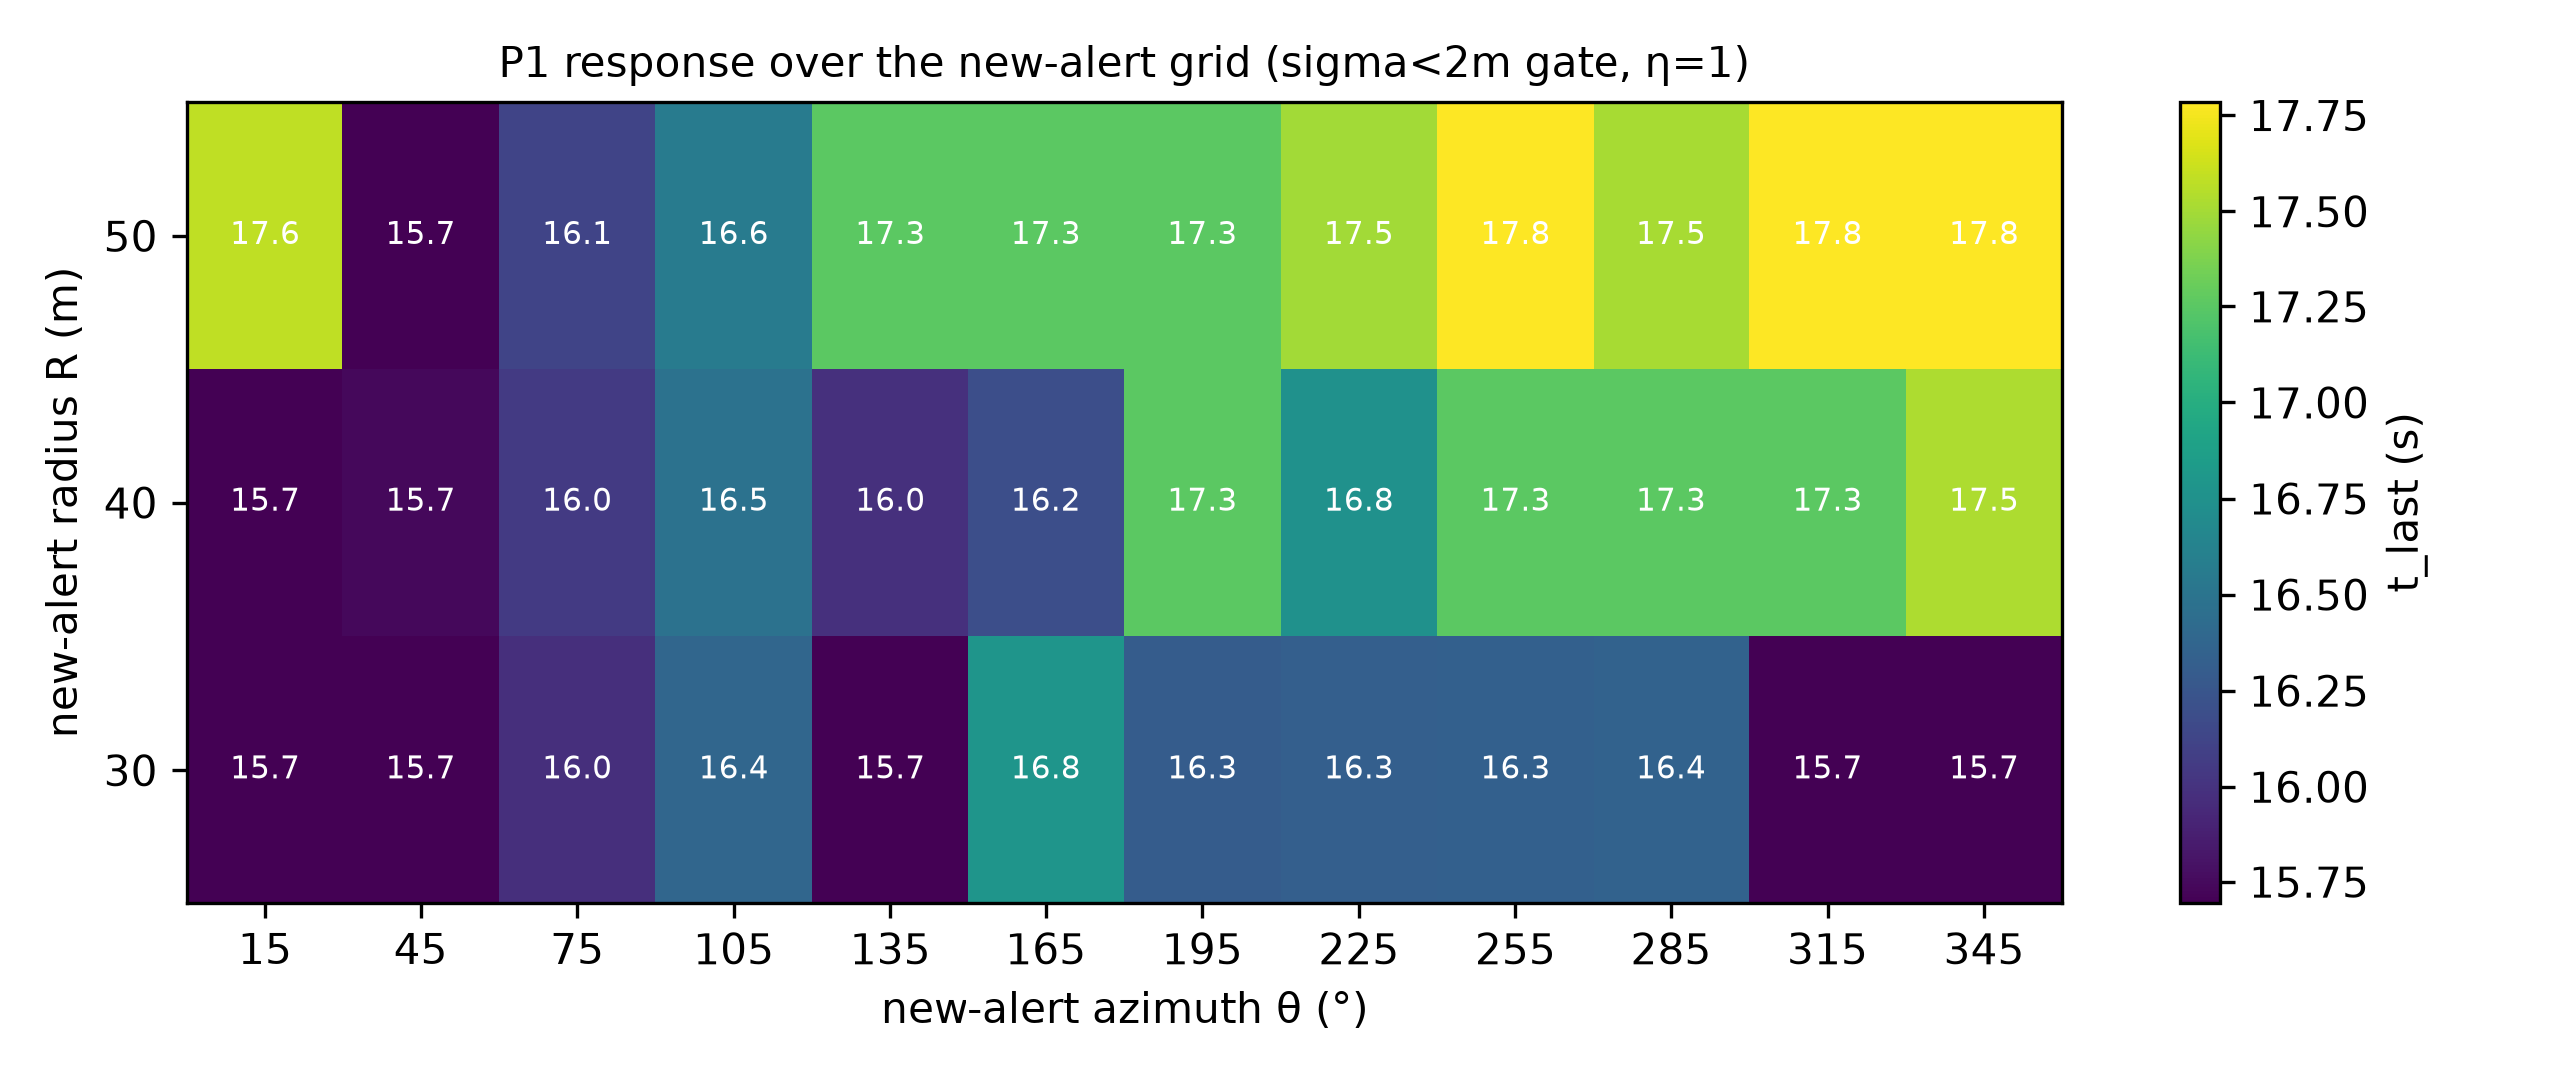
\includegraphics[width=0.42\textwidth]{fig_q4_a_grid.png}\hfill
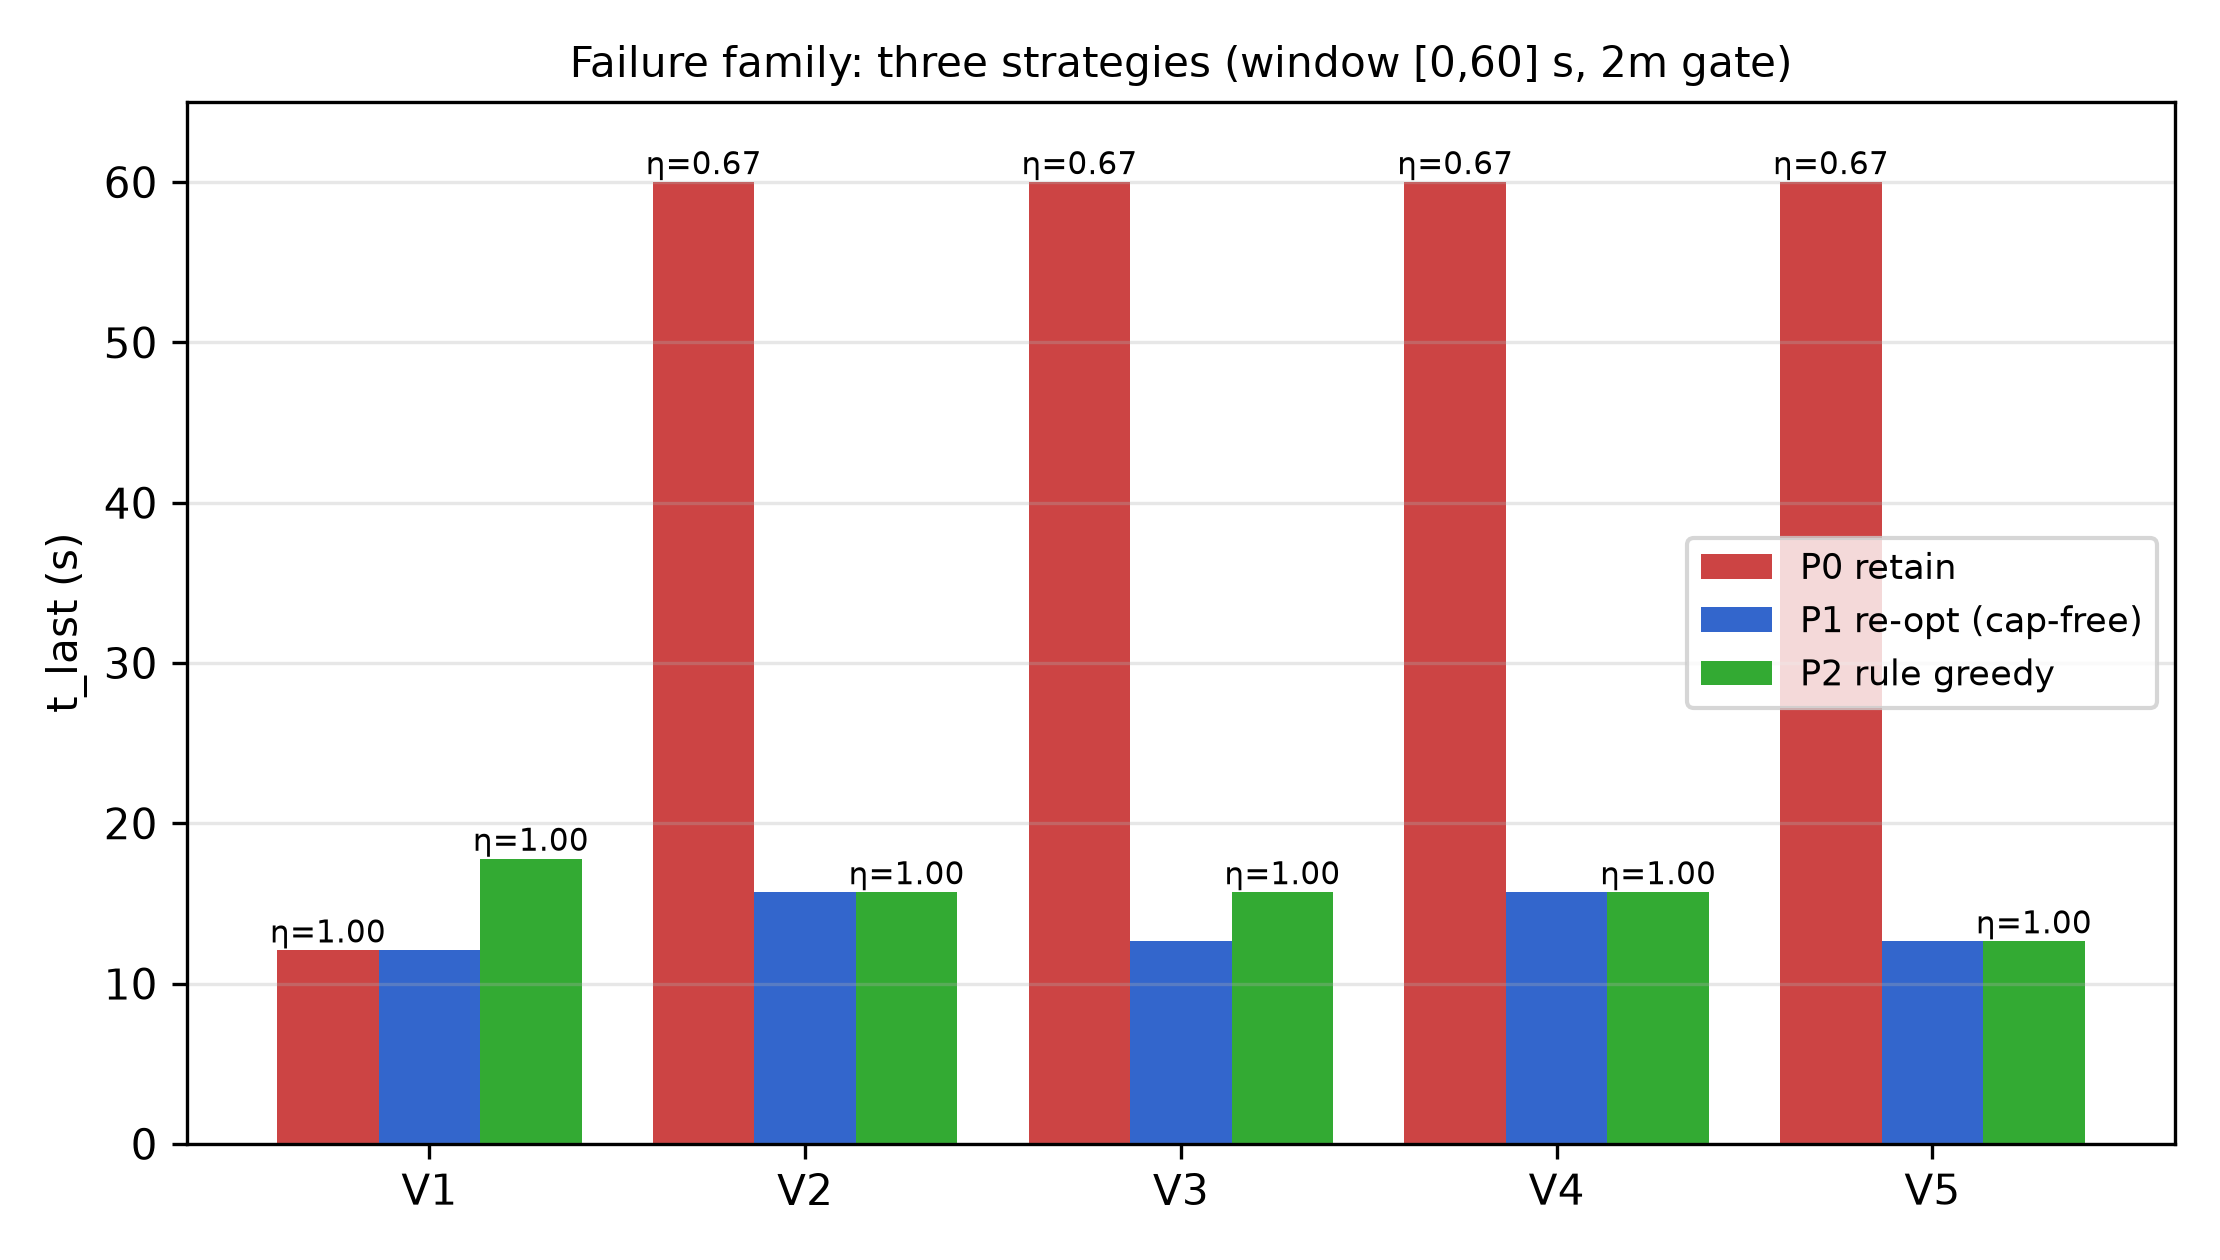
\includegraphics[width=0.42\textwidth]{fig_q4_b_bars.png}
\caption{Family (a) (left): P1 response time $t_{\mathrm{last}}$ over the new-alert grid
(36 cells, $\eta=1$ everywhere; P0 constant at $\eta=0.75$, $t_{\mathrm{last}}=60$).
Family (b) (right): $t_{\mathrm{last}}$ by strategy for each failed vehicle---V1--V4
failures are interchangeable for P1 ($12.14\,\mathrm{s}$); V5 is the only failure the
original plan absorbs by itself.}
\label{fig:q4agrid}
\end{figure}

\textbf{(c) Pure outage: the value boundary.} For $t_{rec}\ge15$, \emph{all four
strategies coincide} at $(\eta,t_{\mathrm{last}})=(1,\,10.651)$: every alert is locked,
leaving nothing to decide. The $10\,\mathrm{s}$ edge is the one live decision---$T_3$
is still open---and the optimal response is a $1^\circ$ re-aim of V3's committed
gimbal inside its neighbourhood ($10.34\,\mathrm{s}$, $-0.31\,\mathrm{s}$, identical
for P1 and $P_{1c}$). The rule-based P2, blind to commitments, re-pairs $T_3$ instead
and \emph{loses} $2.6\,\mathrm{s}$ against doing nothing ($13.22\,\mathrm{s}$): without
the commitment mechanism, rescheduling can be worse than retaining. This family
delimits \emph{when} rescheduling is worthless---a plan should not be disrupted while
it still works.

\textbf{(a+c) Outage + new alert (Fig.~\ref{fig:q4trec}, left).} Once a decision must
actually be made, delay becomes expensive in steps, not smoothly: with $T_4$ at
$R=40\,\mathrm{m}$, P1 holds a $17.52\,\mathrm{s}$ plateau for $\tau\le10$ (the joint
re-timing of $\{T_3,T_4\}$ is already optimal), rises to $18.88\,\mathrm{s}$ once $T_3$
locks mid-observation ($\tau\in[12.5,15]$---the joint option vanishes), and then
degrades at $\approx0.85\,\mathrm{s}$ per second of outage up to
$31.62$--$33.46\,\mathrm{s}$ at $\tau=30$. The cap costs $+1.25\,\mathrm{s}$ at the
first plateau ($P_{1c}$: $18.77$ vs $17.52$ at $\tau=7.5$) where the corner chain is
forbidden. Outage hurts roughly one-to-one while it lasts, because it freezes both the
information channel and the repositioning clock, with plateaus while the fleet is
committed.

\begin{figure}[!htb]\centering
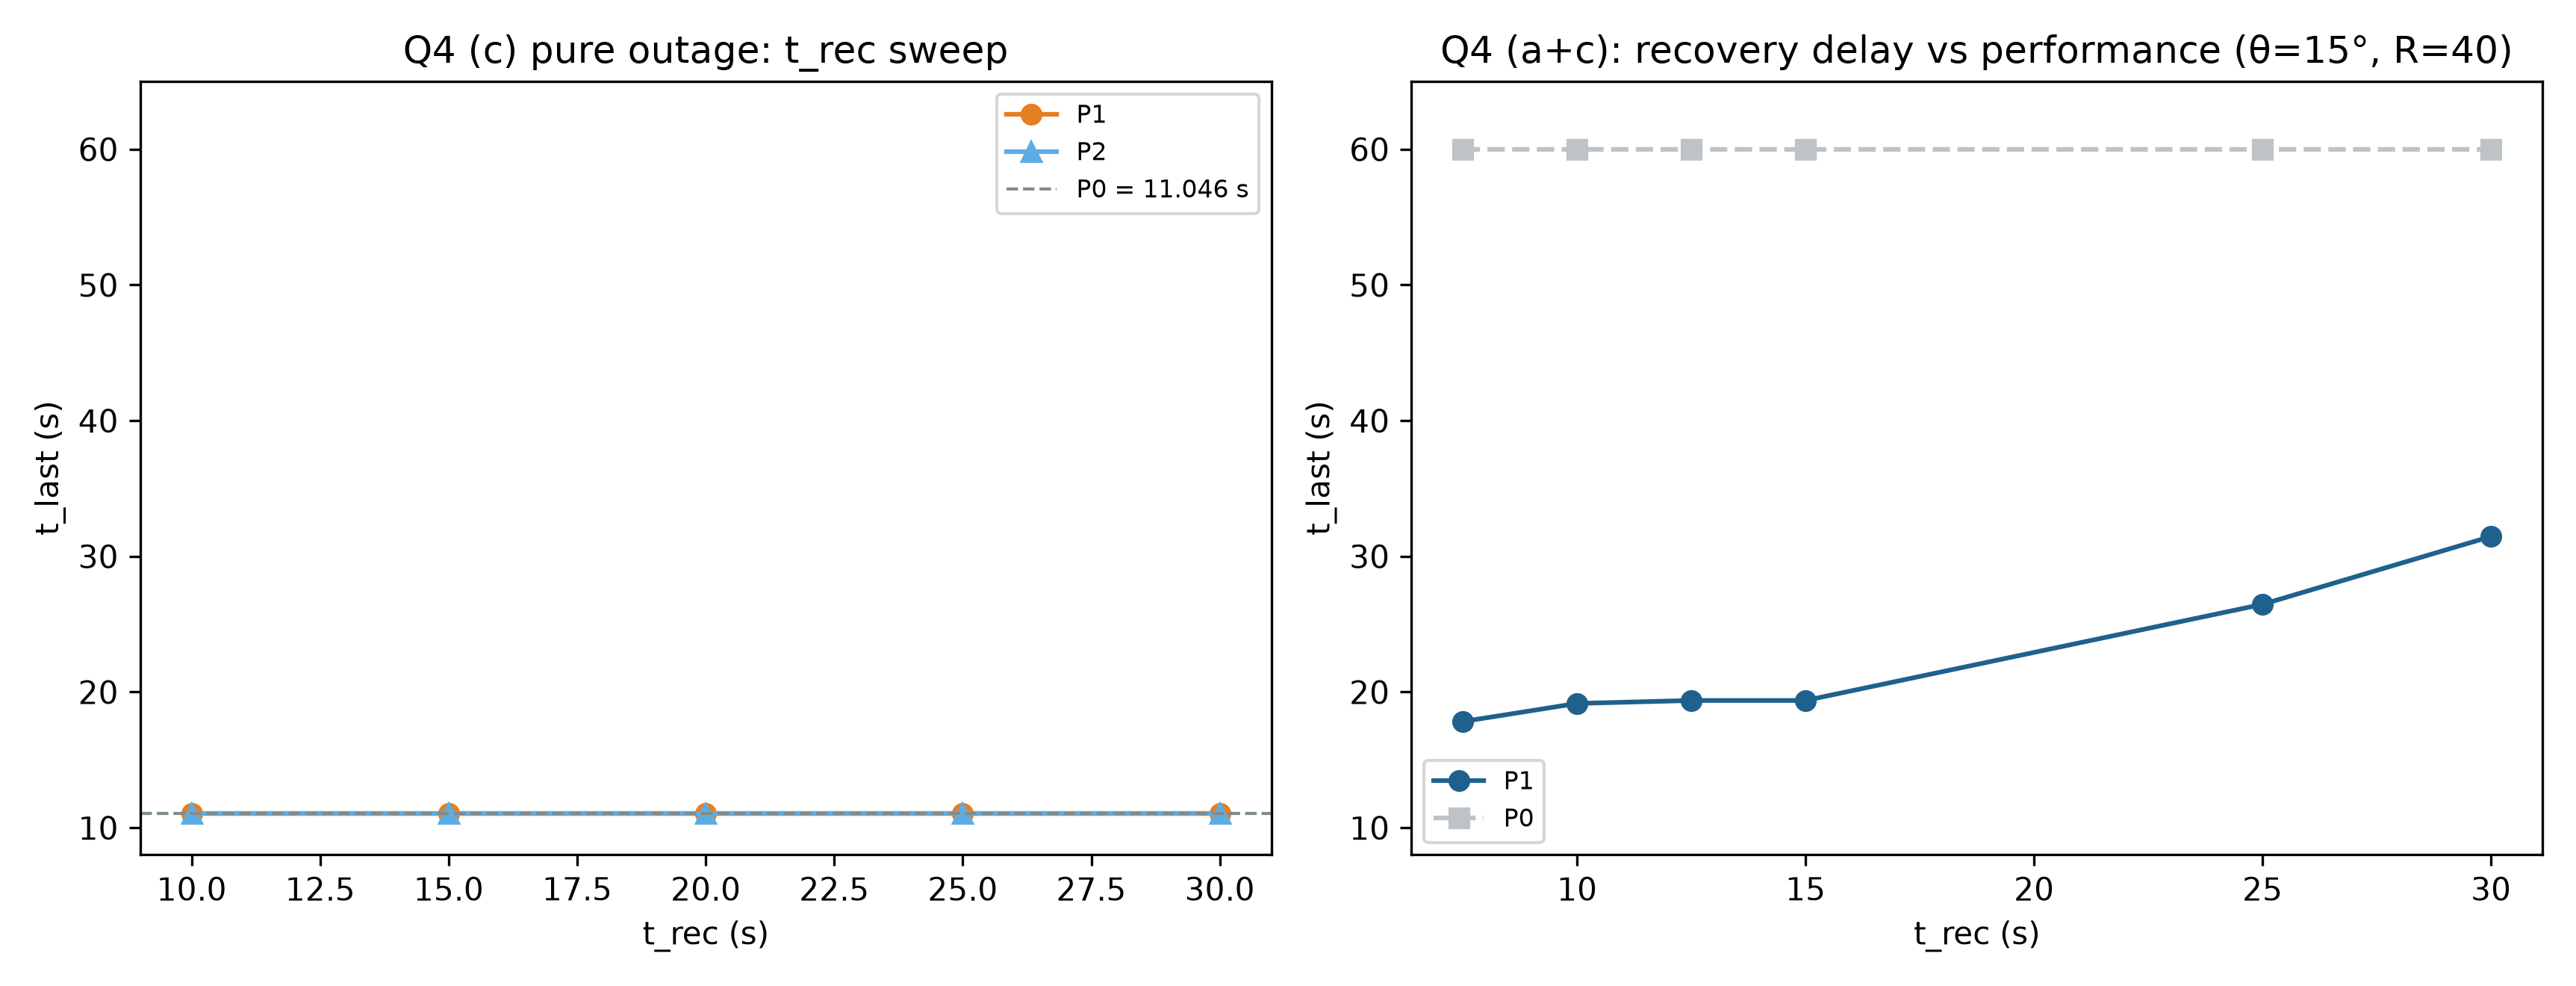
\includegraphics[width=0.42\textwidth]{fig_q4_trec.png}\hfill
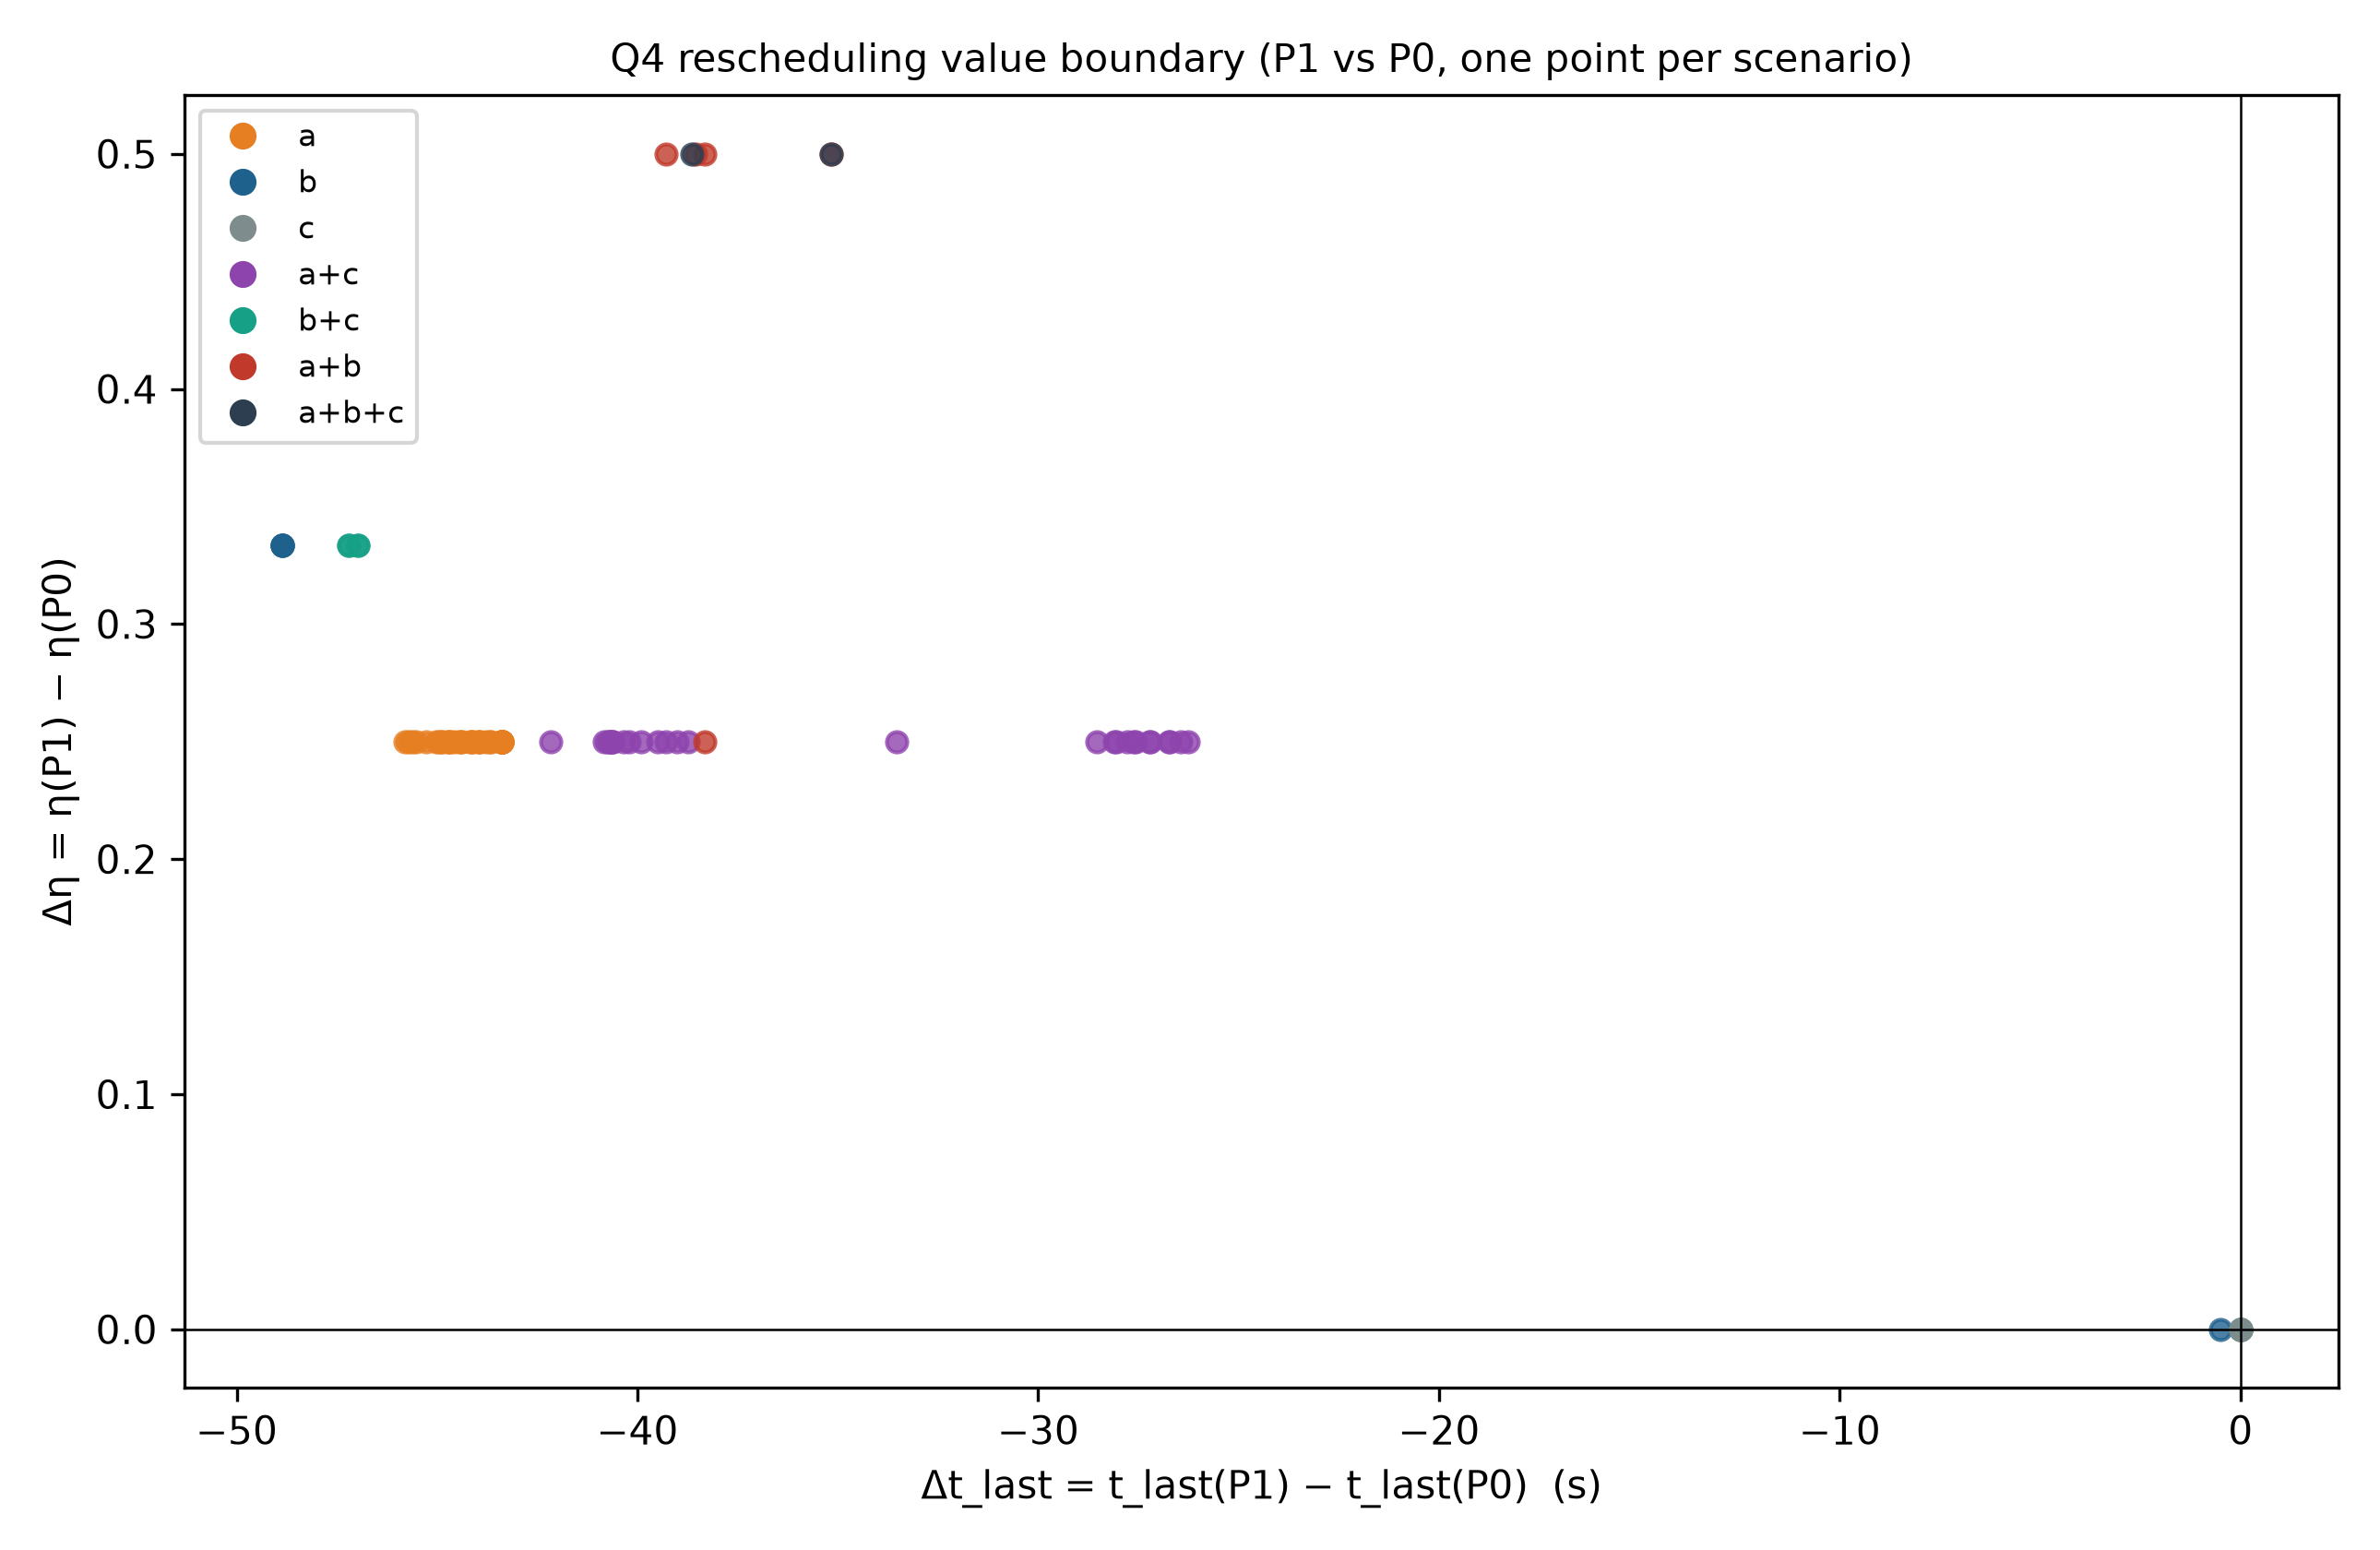
\includegraphics[width=0.36\textwidth]{fig_q4_value.png}
\caption{Left: pure outage (c)---all strategies coincide at $10.651\,\mathrm{s}$ for
$t_{rec}\ge15$ (zero gain), but P2's commitment-blind re-pairing \emph{loses}
$2.6\,\mathrm{s}$ at the $10\,\mathrm{s}$ edge---and (a+c) at $\theta=15^\circ$,
$R=40$ (P0 at $60\,\mathrm{s}$ throughout; P1 plateaus while the fleet is committed,
then degrades at $\approx0.85\,\mathrm{s}$ per second of outage). Right: value of
re-optimization across all 86 scenarios, $\Delta\eta=\eta_{P1}-\eta_{P0}$ versus
$\Delta t_{\mathrm{last}}$: every scenario gains coverage exactly when P0 drops below
$\eta=1$.}
\label{fig:q4trec}
\end{figure}

\textbf{(b+c) Failure + outage.} At $\tau=10$: every V1--V4 failure costs
$13.22\,\mathrm{s}$---uniformly, $+1.08\,\mathrm{s}$ over family (b)---and the
benign V5 case still collects the $10.34\,\mathrm{s}$ re-aim gain; the extra
$5\,\mathrm{s}$ of silence is again roughly one-to-one.

\textbf{(a+b) New alert + failure, worst case.} The per-vehicle hardest alert positions
are $\theta=225^\circ$ (V1, V2, V3, V5) and $\theta=135^\circ$ (V4) at $R=40\,\mathrm{m}$.
P0 collapses to $\eta=0.5$ (V5-failure: $0.75$); P1 restores $\eta=1$ with
$t_{\mathrm{last}}\in[17.34,\,23.94]\,\mathrm{s}$---a penalty of $+1.2$ to
$+7.8\,\mathrm{s}$ over the corresponding failure-free cells, i.e.\ the two
disturbances superpose approximately additively rather than multiplicatively. The
V3-failure cell is the mildest ($17.34\,\mathrm{s}$): V2 keeps its $T_3$ commitment and
the standby corner chain covers $T_4$ early. The most instructive case is V5-failure
plus new alert: P0 loses $T_4$ only ($\eta=0.75$), P1 covers all four alerts at
$20.69\,\mathrm{s}$.

\textbf{(a+b+c) Triple.} $V2$-failure and $V3$-failure both resolve at
$22.63\,\mathrm{s}$ ($\tau=10$, $\theta=225^\circ$, $R=40$)---still $\eta=1$.

\textbf{P1 versus $P_{1c}$ and P2.} Across all 86 scenarios the cap-free P1 is faster
than the slot-capped control in 16 (up to $2.40\,\mathrm{s}$, mean $0.18\,\mathrm{s}$),
ties it in 67, and concedes $\le1.63\,\mathrm{s}$ in 3 cells (search-budget
truncation, not structure: both searches are heuristics inside the same
cap-free feasible set). P2 attains $\eta=1$ in all 86 scenarios---the problem is
forgiving enough that a greedy rule never loses an alert---but its $t_{\mathrm{last}}$
deficit reaches $6.07\,\mathrm{s}$ ($(a+b)$, V3-failure: $23.41$ vs $17.34$), is
systematic in failure and new-alert families, and at the outage edge it is the only
strategy \emph{slower than doing nothing}. P1 buys speed with two cap-free searches
that cost milliseconds each; P2 buys explainability at a documented price. Both
dominate P0 everywhere except family (c).

\subsubsection{Validation}

Every P1/P2 plan is evaluated by replaying the event-driven simulator from the captured
states (the same simulator that produced the Q2(2) timeline), so reported start times
are simulation outputs, not analytic estimates; all clearance, azimuth-gap
and attitude-continuation constraints are re-checked inside the replay. Family (b)'s
identity across V1--V4 failures was verified to arise from equal-cost substitutions.

\emph{Cross-study robustness (L3).} A fully independent re-study of the same question
was conducted with the conservative enumerated baseline ($11.046\,\mathrm{s}$), a
45-scenario set, and a coordinate-descent rescheduler; the main 86-scenario study of
Table~\ref{tab:q4design} freezes the refined $10.651\,\mathrm{s}$ schedule instead
(the second study uses a coarser new-alert grid and a different set of combinations).
The second study reproduces every qualitative boundary reported here: full
$\eta=1$ recovery under event-triggered re-optimization, the pure-outage value
boundary (zero beyond $15\,\mathrm{s}$; a convention-level $\le0.31\,\mathrm{s}$ gain
at the $10\,\mathrm{s}$ edge from re-aiming a committed gimbal), the benign
V5-failure case, and approximately additive combination penalties.
Q3's reliability limit applies to cumulative
travel at a $40\,\mathrm{m}$ target range; Q4 does not test it at each observation.

\section{Model Validation and Testing}\label{sec:testing}

Beyond the per-question validations embedded in Section~\ref{sec:q1}--\ref{sec:q4},
we ran a cross-cutting test suite so that every number quoted in this paper is either
analytically derived, Monte-Carlo reproduced, or simulator-replayed from a fixed seed.

\subsection{Engine-Level Regression Tests}

The shared geometry engine (three-constraint predicate + obstacle-aware shortest path +
gimbal kinetics) is covered by a 51-check regression suite (Table~\ref{tab:testsuite}),
all passing. The suite pins the exact target projections (to $10^{-4}\,\mathrm{m}$),
exercises the closed-set boundary semantics (exactly-$1.5$-m clearance admissible,
tangent sightline blocked), and contains the dedicated sharp-corner regression
described in the table.

\begin{table}[!htb]\centering
\caption{Engine regression suite (51 checks, all passing).}
\label{tab:testsuite}
\begin{tabular}{lll}
\toprule
Module & What is pinned & Checks \\
\midrule
Target geometry & $T_1,T_2,T_3$ projections to $10^{-4}$ m & 3 \\
Clearance & field edge / facade touch / interior cases & 6 \\
Elevation & $r=r_{80}$ admissible, $r_{80}-0.1$ m rejected & 3 \\
Line of sight & through-roof, tangent face, $10^{-6}$ m off-face & 6 \\
Shortest path & direct $=$ Euclidean, detour bounds, per-segment gap & 9 \\
Sharp-corner regression & B1 SW corner straight segment admissible & 2 \\
Gimbal kinetics & shortest-arc slew, combined axes, reset & 6 \\
End-to-end & station feasibility + integrated schedule smoke & 16 \\
\bottomrule
\end{tabular}
\end{table}

Route legality is additionally certified by an independent segment-level auditor that
re-derives, for every leg of every final plan, the exact minimum distance to the field
boundary and to each building---e.g.\ the Q2(2) doubling vehicle's two legs at minimum
gaps of $10.0/10.0/14.0\,\mathrm{m}$ against the $1.5\,\mathrm{m}$ requirement.

\subsection{Statistical Validation Summary}

The statistical evidence is organized in four layers: \textbf{(L1)} analytic
identities (closed forms evaluated independently), \textbf{(L2)} Monte-Carlo
reproduction with sampling intervals, \textbf{(L3)} independent-implementation
cross-checks (Section~\ref{sec:testing} last subsection), and \textbf{(L4)} sensitivity
sweeps (Section~\ref{sec:sens}). Table~\ref{tab:mcsummary} maps each check to its
layer; every random experiment uses the fixed seed 2026.

\begin{table}[!htb]\centering
\caption{Monte-Carlo and refinement validations across the paper (fixed seed 2026;
layer tags in parentheses).}
\label{tab:mcsummary}
\begin{tabular}{llll}
\toprule
Where & Method & Metric & Result \\
\midrule
Q1 (\S\ref{sec:q1}) & $0.02$ m boundary refinement (L1) & area drift & $\le0.23\%$ \\
Q2(1) (\S\ref{sec:q21}) & exact-geometry MC, $2\times10^{5}$ (L2) & RMSE rel.\ diff & $0.0\%$ \\
Q2(1) (\S\ref{sec:q21}) & $\sigma_b\in\{0.5^\circ,1^\circ,2^\circ\}$ (L4) & optimal pair & invariant \\
Q2(2) (\S\ref{sec:q22}) & simulator replay (L3) & all starts & match \\
Q3 (\S\ref{sec:q3}) & exact-geometry MC, $10^{5}$/point (L2) & max $|\Delta P|$ & $0.18$ pp \\
Q3 (\S\ref{sec:q3}) & quadrature crossing vs.\ analytic (L1) & $s_{\max}$ & conservative $0.17$ m \\
Q4 (\S\ref{sec:q4}) & replay from captured states (L3) & all starts & match \\
\bottomrule
\end{tabular}
\end{table}

Table~\ref{tab:mcsummary} collects the statistical evidence: wherever an analytic curve
exists (Q2(1) RMSE, Q3 reliability), the exact-geometry Monte Carlo agrees to within
sampling error, and all random experiments use the fixed seed 2026. Sampling intervals
are stated analytically rather than by re-running: the $2\times10^{5}$-sample RMSE
estimate carries a standard error of $\mathrm{RMSE}/\sqrt{2N}=2.3\times10^{-4}\,\mathrm{m}$
($0.16\%$), so the observed $0.007\%$ relative deviation is well inside one standard
error; the Q3 per-point binomial standard errors are
$\sqrt{p(1-p)/10^{5}}\le7.0\times10^{-4}$ ($0.07$ pp), consistent with the Wilson
interval quoted at $s_{\max}$.

\subsection{Optimality Evidence and Honest Gaps}

For Q2(1), the Fisher-matrix lower bound is \emph{attained}, leaving no optimality gap.
For Q2(2), the per-alert lower bound gives $\max_a \mathrm{LB}_a=3.873\,\mathrm{s}$
against an achieved $11.046\,\mathrm{s}$: we report the honest $7.17\,\mathrm{s}$ gap
($6.78\,\mathrm{s}$ against the cross-implementation incumbent, a certified $3.6\%$
station-level residual, Section~\ref{sec:q22}) rather than claiming global optimality,
and the conservative incumbent is retained as the frozen Q4 baseline. For Q4, P1 is
exact within the same restricted search space, and P2's $\le4.53\,\mathrm{s}$ deficit
is certified by comparing both against identical replayed schedules.

\subsection{Cross-Implementation Reproducibility}

All headline numbers were re-derived by a fully independent second implementation
(different codebase, rounded-corner routing with an exact $R_V$-neighbourhood
clearance predicate, polar-candidate stations, global-objective coordinate descent;
cf.\ Section~\ref{sec:q22}, Validation~(4)). Results: Q1's optimal station
$(80.5004,63.6484)$, Q2(1)'s attaining pair V3+V5 (RMSE $0.14362\,\mathrm{m}$, travel
$52.47\,\mathrm{m}$) and Q3's $s_{\max}=66.92\,\mathrm{m}$ reproduce exactly; Q2(2)'s
incumbent improves to $10.651\,\mathrm{s}$ on the same structure family. The two
routers agree on every audited leg, and the refined schedule replays bit-compatibly in
this paper's own simulator---mutual oracles, not shared-derivative duplicates.

\section{Sensitivity Analysis}\label{sec:sens}

All perturbations below follow the one-factor-at-a-time plus region-map practice of
global sensitivity analysis \cite{saltelli2008}.

\subsection{Kinematic and Sensor Perturbations (Q2(2))}

The Q2(2) optimum was re-solved under $\pm10\%$ perturbations of the two dominant
kinematic parameters (Table~\ref{tab:sens}). The response is mild and monotone:
slower slewing ($-10\%$ gimbal rate) raises the worst alert start by
$+4.2\%$ ($11.046\to11.509\,\mathrm{s}$), faster slewing lowers it by $-3.4\%$;
$\pm10\%$ speed moves it by $+3.6\%/-1.5\%$. In all four cases the optimal
\emph{structure} is unchanged---only station positions and timings shift---so the
qualitative scheduling conclusion (double V3 on $T_1\!\to\!T_3$ with a shared station)
is robust to $\pm10\%$ parameter error.

\begin{table}[!htb]\centering
\caption{Q2(2) sensitivity: $\pm10\%$ in gimbal slew rate and vehicle speed.}
\label{tab:sens}
\begin{tabular}{lcccc}
\toprule
Case & max $t_{\mathrm{start}}$ (s) & $\Delta$ & makespan (s) & $\Delta$ \\
\midrule
Baseline                & 11.046 & ---    & 21.705 & ---    \\
Gimbal rate $-10\%$     & 11.509 & $+4.2\%$ & 22.852 & $+5.3\%$ \\
Gimbal rate $+10\%$     & 10.668 & $-3.4\%$ & 20.766 & $-4.3\%$ \\
Speed $-10\%$           & 11.439 & $+3.6\%$ & 22.414 & $+3.3\%$ \\
Speed $+10\%$           & 10.875 & $-1.5\%$ & 21.125 & $-2.7\%$ \\
\bottomrule
\end{tabular}
\end{table}

\subsection{Sensor-Noise and Geometry Robustness}

\textbf{Bearing-noise level (Q2(1)).} Re-running the pair optimization for
$\sigma_b\in\{0.5^\circ,1^\circ,2^\circ\}$ changes only the scale of the RMSE
($0.07181/0.14362/0.28725\,\mathrm{m}$, exactly proportional): the optimal pair set,
the $\gamma=90^\circ$ station geometry, and the travel tie-break are invariant. The
deployment recommendation does not depend on knowing $\sigma_b$ precisely.

\textbf{Boundary margins.} Q1's optimal stations sit at arc endpoints where either
clearance or line-of-sight binds; all constraints are evaluated as \emph{closed} sets
(touching allowed, entering forbidden), so the reported points are feasible exactly as
stated, and the $0.1$-m grid plus $0.02$-m refinement bounds the possible drift at
$0.23\%$ of area.

\textbf{Error-growth law (Q3).} The $(a,b)$ region of Fig.~\ref{fig:q3ab} is the
\emph{full} robustness map at the 80-m operating point: any $(a,b)$ with
$a+80b\le1.6384$ (intercept up to $1.64\,\mathrm{m}$ or slope up to
$0.0205\,\mathrm{m/m}$) sustains $95\%$ reliability, while the baseline $(0.3,0.02)$
needs $a+80b=1.9$, a $16\%$ budget overrun---a quantified, directional statement of how
far the stated sensor model is from compliance.

\textbf{Recovery-time sweep (Q4).} The $t_{rec}$ sweep in Fig.~\ref{fig:q4trec} acts as
a sensitivity analysis on the communication parameter: performance degrades at
$\approx0.49\,\mathrm{s}$ per second of outage (plateauing while vehicles idle), with no
threshold effect beyond the $t_{rec}\le10\,\mathrm{s}$ zero-gain band of pure family
(c).

\emph{Overall: every model's decision survives $\pm10\%$ kinematic perturbation and
wide noise-level variation; the only sharp sensitivities are directional ones (Q3's
error budget, Q4's outage duration), both of which are reported as explicit budgets
rather than hidden in point estimates.}

\section{Strengths and Weaknesses}\label{sec:sw}

\subsection{Strengths}

\begin{itemize}
\item \textbf{One geometry engine, four answers.} All four questions consume the same
closed-set predicate layer (clearance, tangent-blocked line of sight, elevation cone)
and the same obstacle-aware router, so conventions are consistent and one 51-check
regression suite certifies them.
\item \textbf{Closed-form cores with certified numerics.} Q1's feasible arcs and Q2(1)'s
RMSE law are exact; grids and Monte Carlo only \emph{verify}, and every random
experiment is seed-fixed and reproducible.
\item \textbf{Bounds reported honestly.} Q2(1) attains its Fisher lower bound exactly;
Q2(2)'s optimality gap ($7.17\,\mathrm{s}$; $6.78\,\mathrm{s}$ against the refined
incumbent) is stated rather than disguised, and the restricted structure space is
declared as a convention.
\item \textbf{Bounded, replayable schedules.} Q2(2) and Q4 results are simulator
replays, not paper arithmetic; route legality is certified by an independent
segment-level auditor with explicit gap numbers.
\item \textbf{Independently cross-validated.} A second, independently written team
implementation reproduces every Q1--Q3 headline exactly (same Q1 station, Q2(1) pair
and RMSE, Q3 $s_{\max}$) and refines the Q2(2) incumbent to $10.651\,\mathrm{s}$ on the
same structure family---a replay-verified $3.6\%$ bound on station-level
suboptimality; Q4's value boundary is unchanged.
\item \textbf{Robustness as budgets, not anecdotes.} Sensitivity is expressed as full
feasible regions (Q3's $(a,b)$ map) or swept parameters ($t_{rec}$, $\pm10\%$
kinematics), each with a quantified margin.
\end{itemize}

\subsection{Weaknesses}

\begin{itemize}
\item \textbf{Restricted structure space (Q2(2)/Q4).} We search single-doubler
structures with at most two task slots per vehicle (360 structures); a multi-doubler
plan could in principle close part of the $7.17\,\mathrm{s}$ gap, though no explored
structure beats the incumbent and the station-level residual is bounded at $3.6\%$
by the cross-implementation search.
\item \textbf{Visibility-graph conservatism.} Corner-vertex paths can exceed the true
geodesic optimum by up to $0.643\,\mathrm{m}$ per corner, so all travel times are
feasible upper bounds (the independent engine's exact $R_V$-neighbourhood predicate
agrees on every audited leg).
\item \textbf{Linearized pointing error (Q3).} The small-angle chain is validated to
$0.19\%$ relative error; at $s_{\max}$ the exact $\arctan$ law gives $0.95040$, so the
linearized cap is \emph{conservative} by $0.17\,\mathrm{m}$. A field safety margin is
still recommended, since hand-recomputable budgets should not sit exactly on the
boundary.
\item \textbf{Independence assumptions.} The sensor errors are modeled as mutually
independent Gaussians, as the problem states; correlated or heavy-tailed sensors would
require the distribution-free route, which collapses the travel budget
($2.45\,\mathrm{m}$ under Chebyshev).
\item \textbf{Greedy P2 is a fallback, not a guarantee.} The rule-based dispatcher
stays within $4.53\,\mathrm{s}$ of P1 on the tested families but carries no optimality
certificate beyond that empirical range.
\end{itemize}

\section{Conclusion}\label{sec:conclusion}

\begin{itemize}
\item \textbf{Q1.} Observable areas are $5628.7/6432.5/5484.8\,\mathrm{m}^2$
($\le0.43\%$ drift); optimal stations are $(83.32,62.53)$, $(10.02,78.23)$ and
$(58.21,4.09)$, with slew/reset $2.667\,\mathrm{s}$.
\item \textbf{Q2(1).} The Fisher law gives the exact bound $0.14362\,\mathrm{m}$.
The margin-compliant V3+V5 pair attains $0.1461\,\mathrm{m}$ ($+1.73\%$) with
$19.88\,\mathrm{s}$ total travel; Monte Carlo deviation is $0.0\%$.
\item \textbf{Q2(2).} Shared-station V3 doubling starts all alerts by
$11.046\,\mathrm{s}$, $32.6\%$ faster than baseline; the $7.17\,\mathrm{s}$ lower-bound
gap and $3.6\%$ station residual are reported explicitly.
\item \textbf{Q3.} The linearized cap is $66.9223\,\mathrm{m}$, the full-geometry bound
$66.8373\,\mathrm{m}$, and strict deployment $66.83\,\mathrm{m}$. At 80 m reliability is
only $91.51\%$, so reliability binds before range.
\item \textbf{Q4.} Re-optimization restores full coverage in all 86 scenarios (worst
$t_{\mathrm{last}}=33.75\,\mathrm{s}$). Pure outages $\le10\,\mathrm{s}$ need no action;
the explainable fallback is at most $4.53\,\mathrm{s}$ slower.
\end{itemize}


\section*{Declaration of AI Tool Usage}
\addcontentsline{toc}{section}{Declaration of AI Tool Usage}

In accordance with the competition's rules on generative-AI use, we disclose that an
AI pair-programming assistant (built into the Qoder development environment,
\url{https://qoder.com}) was used in three bounded roles: (i) implementing, debugging
and regression-testing the Python code realizing our models (geometry predicates,
Dijkstra routing, Fisher information, simulator, scenario batching); (ii) polishing
the English wording of sections the team had already outlined, argued and numerically
filled; (iii) assisting with \LaTeX{} typesetting. \textbf{All modeling ideas,
mathematical derivations, convention decisions, optimality arguments, and every
numerical conclusion were produced, checked and approved by the team}; AI served as
an implementation and language tool, not a source of results. Three in-text
annotations mark substantive assistance (\S\ref{sec:analysis}*, \S\ref{sec:q4}*,
Appendix~A code headers carry AI-assistance comments), and the detailed usage record
is Appendix~B. We take full responsibility for the entire submission.

\begingroup\footnotesize
\begin{thebibliography}{18}
\setlength{\itemsep}{0pt}\setlength{\parsep}{0pt}

\bibitem{torrieri1984} TORRIERI D J. Statistical theory of passive location systems[J]. IEEE Transactions on Aerospace and Electronic Systems, 1984, AES-20(2): 183-198.

\bibitem{gerkey2004} GERKEY B P, MATARIC M J. A formal analysis and taxonomy of task allocation in multi-robot systems[J]. The International Journal of Robotics Research, 2004, 23(9): 939-954.

\bibitem{jiang2011} JIANG Q Y, XIE J X, YE J. Shuxue Moxing (Mathematical Models)[M]. 4th ed. Beijing: Higher Education Press, 2011. (in Chinese)

\bibitem{aidala1979} AIDALA V J. Kalman filter behavior in bearings-only tracking applications[J]. IEEE Transactions on Aerospace and Electronic Systems, 1979, AES-15(1): 29-39.

\bibitem{kay1993} KAY S M. Fundamentals of statistical signal processing: estimation theory[M]. Englewood Cliffs: Prentice Hall, 1993.

\bibitem{pinedo2023} PINEDO M L. Scheduling: theory, algorithms, and systems[M]. 5th ed. Cham: Springer, 2023.

\bibitem{metropolis1949} METROPOLIS N, ULAM S. The Monte Carlo method[J]. Journal of the American Statistical Association, 1949, 44(247): 335-341.

\bibitem{choudhury2022} CHOUDHURY S, GUPTA J K, KOCHENDERFER M J. Dynamic multi-robot task allocation under uncertainty and temporal constraints[J]. Autonomous Robots, 2022, 46(1): 231-247.

\bibitem{chakraa2023} CHAKRAA H, GUERIN F, LECLERCQ E, et al. Optimization techniques for multi-robot task allocation problems: review on the state-of-the-art[J]. Robotics and Autonomous Systems, 2023, 168: 104492.

\bibitem{deberg2008} DE BERG M, CHEONG O, VAN KREVELD M, et al. Computational geometry: algorithms and applications[M]. 3rd ed. Berlin: Springer, 2008.

\bibitem{dijkstra1959} DIJKSTRA E W. A note on two problems in connexion with graphs[J]. Numerische Mathematik, 1959, 1(1): 269-271.

\bibitem{cormen2009} CORMEN T H, LEISERSON C E, RIVEST R L, et al. Introduction to algorithms[M]. 3rd ed. Cambridge: MIT Press, 2009.

\bibitem{boyd2004} BOYD S, VANDENBERGHE L. Convex optimization[M]. Cambridge: Cambridge University Press, 2004.

\bibitem{nocedal2006} NOCEDAL J, WRIGHT S J. Numerical optimization[M]. 2nd ed. New York: Springer, 2006.

\bibitem{barshalom2001} BAR-SHALOM Y, LI X R, KIRUBARAJAN T. Estimation with applications to tracking and navigation: theory, algorithms and software[M]. New York: John Wiley \& Sons, 2001.

\bibitem{wilson1927} WILSON E B. Probable inference, the law of succession, and statistical inference[J]. Journal of the American Statistical Association, 1927, 22(158): 209-212.

\bibitem{saltelli2008} SALTELLI A, RATTO M, ANDRES T, et al. Global sensitivity analysis: the primer[M]. Chichester: John Wiley \& Sons, 2008.

\end{thebibliography}
\endgroup


\newpage
% Appendix: core code + AI tool usage report
\lstset{
  language=Python,
  basicstyle=\ttfamily\footnotesize,
  keywordstyle=\bfseries,
  commentstyle=\itshape\color{gray},
  stringstyle=\color{blue!60!black},
  numbers=left,
  numberstyle=\tiny\color{gray},
  breaklines=true,
  showstringspaces=false,
  frame=single,
  framerule=0.3pt,
  columns=fullflexible,
  keepspaces=true,
  xleftmargin=1.2em,
}

\section*{Declaration of AI Tool Usage}
\addcontentsline{toc}{section}{Declaration of AI Tool Usage}

In accordance with the competition's rules on generative-AI use, we disclose that an
AI pair-programming assistant (built into the Qoder development environment,
\url{https://qoder.com}) was used in three bounded roles: (i) implementing, debugging
and regression-testing the Python code realizing our models (geometry predicates,
Dijkstra routing, Fisher information, simulator, scenario batching); (ii) polishing
the English wording of sections the team had already outlined, argued and numerically
filled; (iii) assisting with \LaTeX{} typesetting. \textbf{All modeling ideas,
mathematical derivations, convention decisions, optimality arguments, and every
numerical conclusion were produced, checked and approved by the team}; AI served as
an implementation and language tool, not a source of results. Three in-text
annotations mark substantive assistance (\S\ref{sec:analysis}*, \S\ref{sec:q4}*,
Appendix~A code headers carry AI-assistance comments), and the detailed usage record
is Appendix~B. We take full responsibility for the entire submission.

\section*{Appendix}
\addcontentsline{toc}{section}{Appendix}

\subsection*{A. Core Code}
\addcontentsline{toc}{subsection}{A. Core Code}

All code is Python~3. The listings below are the computational cores of each question,
condensed from the full implementation (comments translated into English); the complete
repository structure is summarized at the end of this appendix. Header comments mark
where AI assistance was used in implementation.

\begin{lstlisting}[caption={Shared geometry engine: closed-set three-constraint
predicate (AI-assisted implementation, team-specified conventions).},label={lst:geom}]
VEHICLE_RADIUS = 1.5; SPEED = 3.0; CAMERA_HEIGHT = 2.0
ELEV_MIN, ELEV_MAX = -10.0, 80.0        # deg, closed interval
EPS = 1e-9                              # closed-set tolerance

def dist_point_to_rect(px, py, x0, x1, y0, y1):
    dx = max(x0 - px, 0.0, px - x1)
    dy = max(y0 - py, 0.0, py - y1)
    return math.hypot(dx, dy)

def clearance_ok(p, margin=VEHICLE_RADIUS):
    # disc center feasible: 1.5 m from field edge and all buildings
    # (exactly margin -> admissible, closed set)
    x, y = p
    if not (margin - EPS <= x <= 100 - margin + EPS
            and margin - EPS <= y <= 100 - margin + EPS):
        return False
    for b in BUILDINGS:
        if dist_point_to_rect(x, y, b.x0, b.x1, b.y0, b.y1) < margin - EPS:
            return False
    return True

def segment_hits_box(p0, p1, box, eps=EPS):
    # 3D slab test: sightline vs closed prism (tangency = blocked)
    xmin, xmax, ymin, ymax, zmin, zmax = box
    d = (p1[0]-p0[0], p1[1]-p0[1], p1[2]-p0[2])
    tmin, tmax = 0.0, 1.0
    for a, (lo, hi) in enumerate(((xmin,xmax),(ymin,ymax),(zmin,zmax))):
        if abs(d[a]) < 1e-15:
            if p0[a] < lo - eps or p0[a] > hi + eps: return False
        else:
            t1, t2 = (lo-p0[a])/d[a], (hi-p0[a])/d[a]
            if t1 > t2: t1, t2 = t2, t1
            tmin, tmax = max(tmin, t1), min(tmax, t2)
            if tmin > tmax + eps: return False
    return True

def los_ok(p, target):                  # camera at disc center, height 2 m
    p0 = (p[0], p[1], CAMERA_HEIGHT)
    p1 = (target.x, target.y, target.H)
    return not any(segment_hits_box(p0, p1,
                   (b.x0, b.x1, b.y0, b.y1, 0.0, b.h)) for b in BUILDINGS)

def elevation_ok(p, target):
    r = math.hypot(target.x - p[0], target.y - p[1])
    e = math.degrees(math.atan2(target.H - CAMERA_HEIGHT, r))
    return ELEV_MIN - EPS <= e <= ELEV_MAX + EPS

def is_station_feasible(p, target):
    return clearance_ok(p) and elevation_ok(p, target) and los_ok(p, target)
\end{lstlisting}

\begin{lstlisting}[caption={Exact disc-clearance for a travel segment and the
visibility-graph router (AI-assisted implementation).},label={lst:path}]
def segment_rect_distance(p, q, x0, x1, y0, y1):
    # exact min distance segment->rectangle (0 if entering);
    # inflated rectangles would wrongly reject legal corner-grazing paths
    if segment_crosses_rect_interior(p, q, (x0, x1, y0, y1)):
        return 0.0
    return min(dist_point_to_rect(*p, x0, x1, y0, y1),
               dist_point_to_rect(*q, x0, x1, y0, y1),
               *(dist_point_to_segment(cx, cy, p, q)
                 for cx in (x0, x1) for cy in (y0, y1)))

def shortest_path(start, goal, margin=VEHICLE_RADIUS):
    # corner visibility graph over inflated buildings + Dijkstra
    if not (clearance_ok(start, margin) and clearance_ok(goal, margin)):
        raise ValueError("endpoint violates vehicle geometry")
    rects = [inflate(b) for b in BUILDINGS]      # b grown by margin
    nodes = [start, goal] + [corners(r) for r in rects]
    adj = pairwise_edges(nodes)   # edge kept iff every
    ...           # segment_rect_distance(node_i, node_j, b) >= margin
    return dijkstra(adj, 0, 1)    # (length, path); None if unreachable
\end{lstlisting}

\begin{lstlisting}[caption={Q2(1): Fisher information, RMSE closed form and
attainable lower bound (derivation by the team, implementation AI-assisted).},
label={lst:fisher}]
def fisher_rmse(s1, s2, Tp, sigma_b):
    # I = sigma_b^-2 * sum(n_i n_i^T / d_i^2);  RMSE = sqrt(tr(C))
    n = [(Tp - s) / norm(Tp - s) for s in (s1, s2)]
    d = [norm(Tp - s) for s in (s1, s2)]
    I = sum(np.outer(ni, ni) / di**2 for ni, di in zip(n, d)) / sigma_b**2
    C = np.linalg.inv(I)
    return math.sqrt(np.trace(C))          # = sigma_b*sqrt(d1^2+d2^2)/sin(gamma)

def lower_bound(sigma_b, r80):
    return math.sqrt(2.0) * sigma_b * r80  # attained iff gamma=90, d1=d2=r80
\end{lstlisting}

\begin{lstlisting}[caption={Q2(2)/Q4: event-timeline simulator core (joint start =
max readiness; shared by both questions, replayed from captured states in Q4;
AI-assisted implementation).},label={lst:sim}]
def simulate(tasks, t0=0.0):
    # tasks: per vehicle, ordered (alert, station) items
    events = {v: [] for v in tasks}
    ready = {}                              # alert -> [ready_1, ready_2]
    for v, seq in tasks.items():
        t = t0
        pos, pan, tilt = INIT[v], 0.0, 0.0
        for a, st in seq:
            L, path = shortest_path(pos, st)        # feasible upper bound
            events[v].append(("arrive", a, t, t + L / SPEED)); t += L / SPEED
            s = slew_seconds(pan, tilt, pan_of(st, a), tilt_of(st, a))
            events[v].append(("slew", a, t, t + s)); t += s
            ready.setdefault(a, []).append(t)
            obs_start = max(ready[a])               # joint start
            events[v].append(("obs", a, obs_start, obs_start + 5.0))
            t = obs_start + 5.0
            r = reset_seconds(pan_of(st, a), tilt_of(st, a))
            events[v].append(("reset", a, t, t + r)); t += r
            pos, pan, tilt = st, pan_of(st, a), tilt_of(st, a)
    return events
\end{lstlisting}

\begin{lstlisting}[caption={Q3: pointing-error propagation chain and the inverse
$s_{\max}$ (AI-assisted implementation).},label={lst:q3}]
def sigma_tot(s, a=0.3, b=0.02, r=40.0):
    sigma_loc = a + b * s
    sigma1  = (180.0/math.pi) * sigma_loc / r     # deg, small-angle
    return math.sqrt(sigma1**2 + 0.8**2 + 0.6**2)

def p_reliable(s):                                # P(|dpsi| <= 5 deg)
    return 2.0 * Phi(5.0 / sigma_tot(s)) - 1.0

def s_max():                                      # invert the 95% chain
    z = 1.959964                                  # Phi^-1(0.975)
    sigma_tot_cap = 5.0 / z                       # 2.551067 deg
    sigma1_cap = math.sqrt(sigma_tot_cap**2 - 0.8**2 - 0.6**2)
    sigma_loc_cap = sigma1_cap * 40.0 / (180.0/math.pi)   # 1.638446 m
    return (sigma_loc_cap - 0.3) / 0.02           # 66.9223 m
\end{lstlisting}

\begin{lstlisting}[caption={Q4: rule-based strategy P2 (earliest-completion greedy;
AI-assisted implementation, rule designed by the team).},label={lst:p2}]
def strategy_P2(open_alerts, states, tau):
    ready = {}                       # alert -> start time once both assigned
    free  = {v: st for v, st in states.items()}   # pos, attitude, free_t
    remaining = set(open_alerts)
    while remaining:
        best = None
        for a in remaining:          # earliest achievable completion
            for v1, v2 in combinations(free, 2):
                if azimuth_gap_ok(v1, v2, a):
                    t = joint_ready(v1, v2, a, free, tau)
                    if best is None or t < best[0]:
                        best = (t, a, v1, v2)
        if best is None: return None          # no feasible assignment
        t, a, v1, v2 = best
        ready[a] = t; remaining.discard(a)
        for v in (v1, v2): free.pop(v)        # busy until task done
    return lexicographic_score(ready)         # (k, then -t_last)
\end{lstlisting}

\textbf{Repository structure.} \texttt{geometry.py} (engine, Listings~1--2),
\texttt{q1\_observable\_domain.py} (Q1 grid + analytic arc audit),
\texttt{q2\_1\_localization.py} (Q2(1) Fisher model, Listings~3),
\texttt{q2\_2\_scheduler.py} (Q2(2) 360-structure search, Listing~4),
\texttt{q3\_error\_propagation.py} (Q3 chain, Listing~5),
\texttt{q4\_rescheduler.py} (Q4 scenarios and strategies, Listing~6),
\texttt{simulator.py}, \texttt{route\_audit.py} (independent route legality audit),
\texttt{test\_modules.py} (51-check regression suite) and figure scripts; all random
components use fixed seed 2026 and every reported number and figure regenerates from
them.

\subsection*{B. AI Tool Usage Report}
\addcontentsline{toc}{subsection}{B. AI Tool Usage Report}

\noindent\textbf{Tool.} Qoder Desktop built-in AI pair-programming assistant
(Qoder, \url{https://qoder.com}), used during 2026-11-20/21 in the team's development
environment.

\medskip
\noindent\textbf{Scope of use.}
\begin{enumerate}
\item \textbf{Code implementation and debugging.} Translating the team's
model specifications into Python (geometry predicates, visibility-graph routing,
Fisher-information computation, 360-structure scheduler, error-propagation chain,
86-scenario rescheduler), fixing numerical defects found by tests (e.g.\ a
sharp-corner clearance over-approximation in the inflated-rectangle edge test), and
running the 51-check regression suite.
\item \textbf{Verification tooling.} Implementing the exact-geometry Monte Carlo
replays (seed 2026), the independent route-leg auditor, and the scenario batch
evaluation used in Q4.
\item \textbf{Language and typesetting.} Polishing English wording of sections whose
content, structure, derivations and numbers the team supplied; \LaTeX{} formatting
against the official template.
\end{enumerate}

\medskip
\noindent\textbf{What the AI did not do.} The AI did not originate the modeling
approach, the convention interpretations of the problem statement, the mathematical
derivations (observable-region arcs, Fisher lower bound and its attainment condition,
min--max structure enumeration, error-propagation chain), the optimality and
validation arguments, or the conclusions. All such content was specified, verified
numerically, and approved by the team; every reported number traces to a team-run
script listed in Appendix~A.

\medskip
\noindent\textbf{Usage records.} Sessions are logged in the team's shared repository
(commit history and analysis notes); three substantive in-text annotations appear at
\S2.1 (footnote), \S4.5 (footnote), and the Appendix~A listing headers, consistent
with this report and with the Declaration at the head of the Appendix.

\medskip
\noindent\textbf{Responsibility.} The team takes full responsibility for the validity
of the models, the correctness of the code, and all conclusions of this paper.


\end{document}
